\chapter{Peg in hole}

In Chapter 3, we demonstrated that we could learn a search policy and successfully transfer it to a robot apprentice
from demonstrations of human teachers for a task consisting of locating a wooden object on a table. 
In these search tasks our approach is based on the fact that intuition and knowledge exhibited by the human teachers, 
during the search, gives a good balance between exploration and exploitation actions which can then be encapsulated in 
a generative Gaussian Mixture Model (GMM) and be subsequently used as a control policy. 
The approach is satisfactory when extracting the many different behaviours demonstrated by the human teachers and reproducing 
them. However for learning an optimal or near optial policy with a unique behaviour the using  
of this approach will not necessarily result in a efficient policy. For the GMM we model
both the good and the bad search strategies exhibited by the human teachers. If the task is difficult and many possible solutions exist, such 
as in the previously discussed blindfolded search task in Chapter 3, many demonstrations will be required for search patters to
emerge and be encoded in the GMM. Otherwise the GMM needs to be combined with another policy as previously shown (Hybrid GMM-Greedy 
policy). 

%  This sentence is hard to follow. Break it into two sentences. What do you mean by goal-oriented? 
%  It is not clear which shortcoming you want to highlight. Is the requirement for consistency or for goal-orientedness? 
% Obviously, any task < no? The consistency requirement is also somewhat contradictory with the fact that you were embedding different 
% styles of search across demonstrations.

GMM does not discriminate between behaviours, as the Expectation-Maximisation (EM) algorithm used to 
learn the GMM policy ignores the quality of the demonstrated data. The EM algorithm does not contain a cost or 
reward function, encoding the objective of the task, which is common practice in Planning and Reinforcement Learning (RL). 
In the case of a difficult task where there are mostly bad demonstrations, the GMM search policy will reproduce suboptimal behaviour.
Additionally there may be that no good teachers, however by combining different components from 
individual demonstrations a good search strategy can be extracted.


%teachers are not good at the task individually and maybe only a few demonstrations are the best, whilst the majority are bad.
%There the task undertaken is implicitly encoded, as there is no cost function which is optimised, in 
%the GMM and as a result the taught behaviour has to be goal oriented and consistent, which is not always the case in a blindfolded search task. 

To overcome the above mentioned limitations, we introduce a binary cost function as a means of ranking the human teachers' demonstrations.
To this end, we combine our PbD-POMDP approach with an Actor-Critic Reinforcement Learning (RL) framework which 
is close to Fitted-Value Iteration(FVI) and other Experience replay methods. This new method we refer to as RL-PbD-POMDP. 
Our objective is to avoid the noisy explorative rollouts, a weakness common to all RL approaches, and only rely on 
the data provided by the human teachers. Autonomous exploration in RL can be seen to have three problem areas.

Firstly it is time consuming and is typically only applicable where an exhaustive exploration 
of the entire state or parameter space is feasible, such as in the inverted pendulum or mountain cart type problems. 
The universal exploration method, used throughout RL, is state independent (sometimes state dependent) white noise 
which results in an entire exploration of the state space. This
is neither practical nor feasible for the type of search problems we are considering. Secondly in this search 
problem as we are using a physical robotic system the exploration cannot be random as this would be dangerous.
Finally it is imperative that both the PbD-POMDP and RL-PbD-POMDP receive the same information. This would enable a fair comparison 
between the two algorithms and support our hypothesis that the RL-PbD-POMDP provides an improved policy 
with only human demonstrations as input.

%We chose a search and Peg-In-Hole (PiH) task
We analyse our RL-PbD-POMDP approach on a power-socket Peg-in-Hole (PiH) search task. In this task, human teachers must demonstrate 
to a robot apprentice how to search for and connect a plug to a power socket, see Figure \ref{fig:experiment_setup} (\textit{Left}). 
The first part of the task, the search for the socket, is similar to the table wooden-block setup in the previous chapter. 
However the connection of the plug to the power socket, the PiH component, requires a higher level of precision.
In Figure \ref{fig:experiment_setup} (\textit{Right}) the robot reproduces the behaviour demonstrated by the teacher.

% Show figure of the task setup.
\begin{figure}[h]
  \centering
  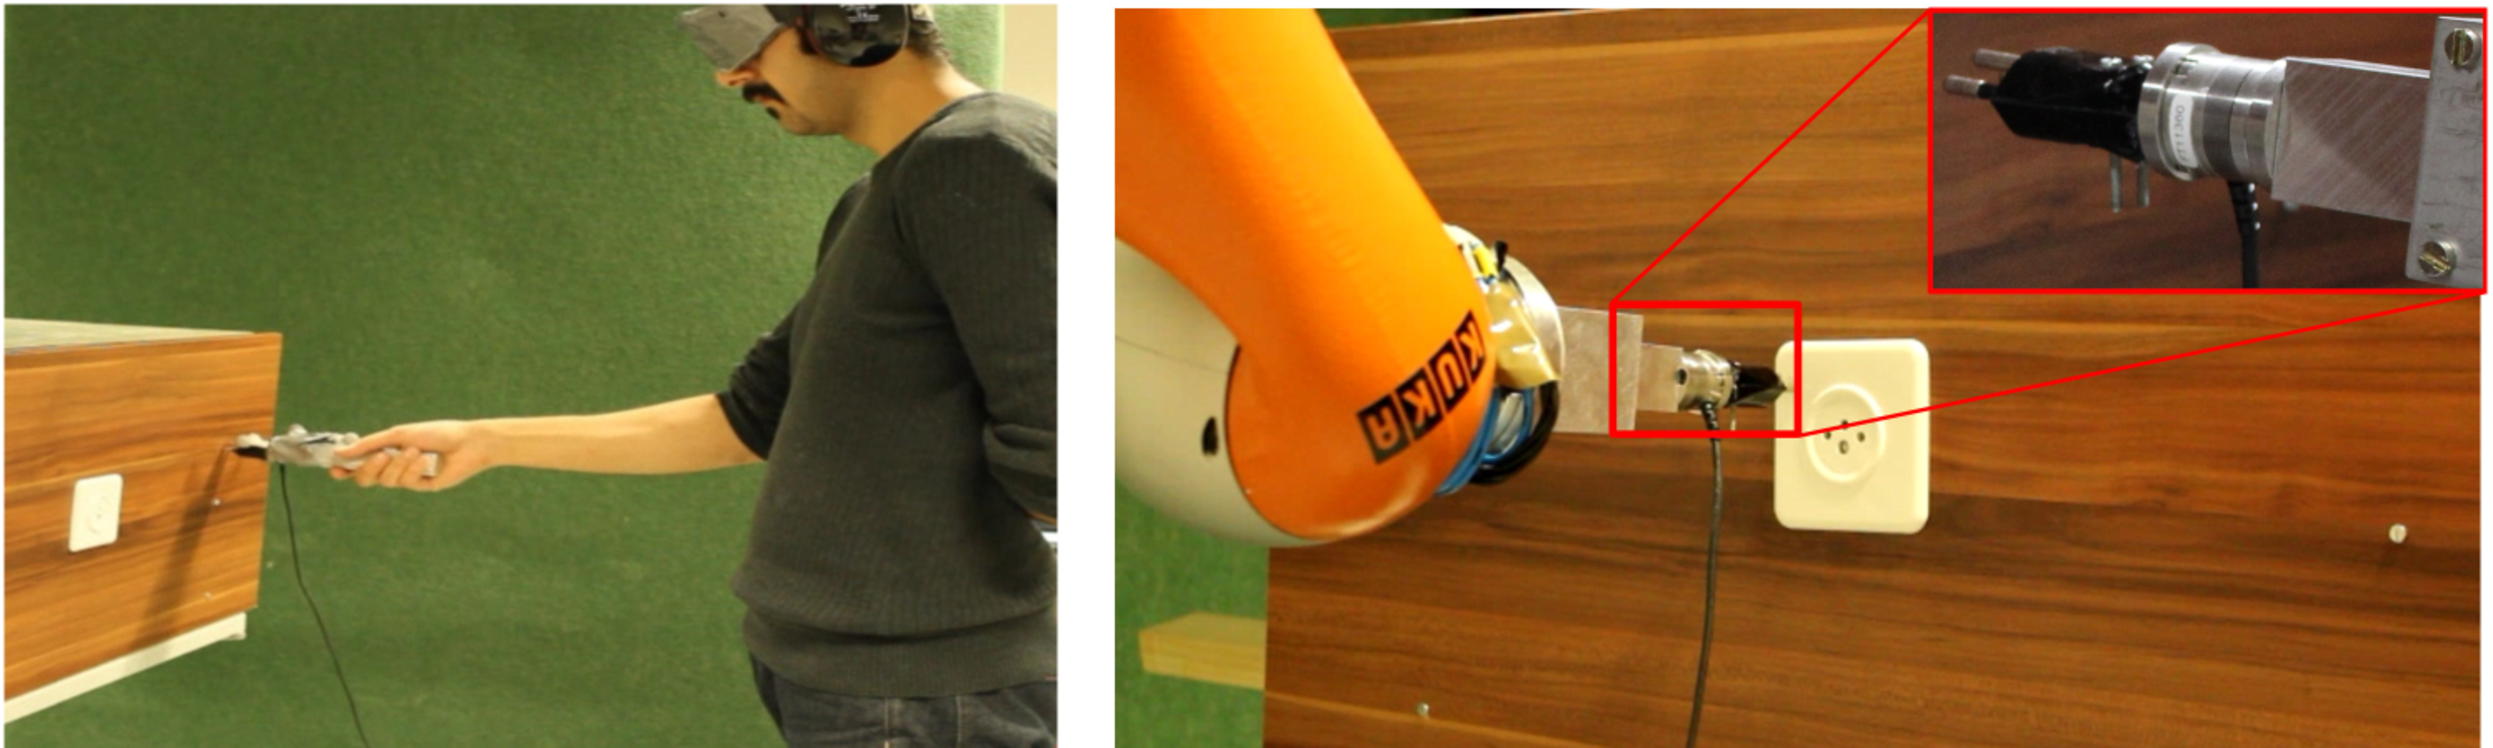
\includegraphics[width=0.95\textwidth]{./ch4-PiH/Figures/Fig/human_example_search.pdf}
  \caption{Peg-in-hole (PiH) search task. \textit{Left:} A teacher is wearing ear defenders (to impede any hearing) and 
  a blindfold. He first searches for the socket's location and then attempts to establish a connection. Force 
  and torque information is obtained from an ATI 6-axis force torque sensor at the end-effector of the tool held by the teacher.
  \textit{Right:} The KUKA LWR4 robot equipped with the same force torque sensor and plug reproducing the teacher's demonstrated behaviour.}
  \label{fig:experiment_setup}
\end{figure}


%(\textit{Top-right}), we illustrate the setup of the search task. The diagram shows
%the distribution of the initial starting position (in orange) of the human teachers. As was the case in our previous search experiment
%in Chapter 3, the teacher is disoriented before each trial but knowns that his initial heading will be the same, facing the wall. 
%The human teachers are deprived of visual information (they are blindfolded) and their hearing sense is significantly 
%reduced (by wearing ear defenders).  
%QIn the \textit{Bottom-left} quadrant we
%can see an example of a human teacher trying to accomplish the search and connection task, and to the \textit{Bottom-right} the KUKA
%LWR robot apprentice is reproducing a search policy learned from the teacher.

\section{Outline}
\begin{itemize}
  \item \hyperref[ch4:background]{\ref{ch4:background}   Background}\\
  We review aspects of the literature related to the Peg-in-hole problem and Actor-Critic Reinforcement Learning 
  with an emphasis on Fitted methods (also known as Batch or Experience replay), which we adapt to our GMM policy.
  \item \hyperref[ch4:experiment]{\ref{ch4:experiment}   Experiment methods}\\
  We detail the Peg-in-Hole search task, the number of participants (teachers) which provide demonstrations, the 
  type of data which is recorded and the representation of the human's location belief.
  \item \hyperref[ch4:learning-value-actor]{\ref{ch4:learning-value-actor} Learning Actor and Critic}\\
  We detail the representation of the Actor and the Critic and how they are learned in a Fitted Policy Evaluation 
  framework.
  \item \hyperref[ch4:control_architecture]{\ref{ch4:control_architecture} Control architecture}\\
  The learned behaviour is demonstrated on a 7 Degree of Freedom (DoF) articulated robot, named KUKA LWR4. 
  We detail the hybrid position-force controller and dynamical field modulation heuristic which is used in 
  combination with the learned behaviour policy from the human teachers.
  \item \hyperref[ch4:results]{\ref{ch4:results}  	 Results}\\
  We perform a set of 5 simulated experiments to test the generalisation, the importance of data provided by the human 
  teachers and the performance against simple search approaches to find the location of the socket. We further perform 
  3 experiments on the real robotic platform to test the generalisation of the learned policy on different power sockets.
  \item \hyperref[ch4:conclusion]{\ref{ch4:conclusion} Conclusion}\\
  The RL-PbD-POMDP policy achieves an important improvement over the previous PbD-POMDP approach
   by learning a value function over the belief space using approximate dynamic programming (part of FVI) and using it 
   to update the parameters of our GMM policy. We evaluate the ability of the policies to generalise to novel sockets 
   and different socket locations, both in simulation and on the KUKA LWR robot.
   The RL-PbD-POMDP approach consistently proves to be better. More importantly the RL-PbD-POMDP approach performs 
   significantly better when it is used on the worst teacher's demonstrations, which mitigates the \textbf{original assumption} that 
   teachers have to be consistently efficient at the task.
\end{itemize}

\section{Background}\label{ch4:background}

\subsection{Peg-in-hole}

The Peg-in-Hole (PiH) task is one of the most widespread step in industrial assembly and manipulations processes, with 
examples including the assembly of vehicular transmission components \cite{search_strategies_icra_2001} and 
valves \cite{online_gpr_icra_2014}. To be successful, the estimated
position of the robot's end-effector and workpiece must be precise. Typically, the clearance between peg and plug 
is very small leaving little room for error. As a result, variations in the assembly's components 
in combination with position uncertainty can result in either jamming during the insertion process or in failure for 
the plug finding the hole. This created a need for adaptive search and insertion policies for PiH, which has been driving research 
in this area. 

From the literature, we identified the different components in PiH solutions. 

All approaches use to some extent a vision system to estimate the position of the workpiece. 
For instance in \cite{peg_personal_icra_2010} a PR2 is equipped with a checkerboard to facilitate pose 
estimation  of the plug with respect to a power outlet whose position is extracted through a vision 
processing pipeline. An initial connection is attempted by visual servoing which is successful 10\% of the 
time. Given an estimate of the workpiece's position, a common approach is to follow either a blind increasing spiral 
Cartesian trajectory or parametrised policies which guarantee that all positions on the workpiece have been visited.
In \cite{peg_personal_icra_2010}, if the PR2 initially fails to connect the plug to the socket
a spiralling outward motion is carried out with 2mm increments which obtains an overall 
success rate of 95\%. For this approach to be applicable to a generic robot, it would require the addition of an
external camera and checkerboard to the robot in question which might be cumbersome. In our work we consider a 
vision free system.

%To increase the chances of a connection these approaches use a compliant controller 
%which usually includes a hybrid force/position controller.
%In \cite{peg_personal_icra_2010} a PR2 executes a parameterised policy designed to connect a plug to a power outlet
%in order for the PR2 to recharge itself. The plug is equipped with a checkerboard to facilitate pose estimation
%of the plug with respect to power outlet whose position is extracted through a vision processing pipeline.
%An initial connection is attempted by visual servoing which is successful 10\% of the time. 
%When unsuccessful a spiralling outward motion is carried out with 2mm increments. 
%This method achieved an overall success rate of 95\%.
%The hybrid control paradigm \cite{hybrid_1992} was used throughout the execution of the task.
%The first approach does not consider reproducing the F/T profile 
%but rather follows a position trajectory whilst being compliant.


Another approach (which has been confined to academic circles) follows the data driven 
Programming by Demonstration (PbD) framework. Teleoperated or kinesthetic demonstrations by a human teacher 
are recorded and a policy is learned and fine-tuned so as to reproduce the same (F)orce/(T)orque profile as 
that demonstrated by the human teacher. 

% PbD: reproduce the F/T profile irrespective of the learned position trajectory DMP
In \cite{fast_peg_pbd_icmc_2014} the authors learn a PiH policy for the Cranfield benchmark object.
A vision system obtains the pose parameters of the object whilst a human teacher  
demonstrates trajectories, through teleoperation, in the frame of reference of the object. 
A time-dependent policy represented with Dynamic Movement Primitives (DMP) \cite{Schaal04learningmovement} 
encodes the recorded Cartesian end-effector pose. In \cite{trans_workpiece_icra_2013}, a F/T profile 
is encoded separately by a regressor parameterised by radial basis functions. Successive refinements of the DMP policy are achieved through 
using force feedback to adapt the parameters of an admittance controller. This results in the policy having
similar force profiles to the human teachers. Further applications based on this method have been 
performed \cite{sol_pdg_pbd_2014} with the incorporation of a disturbance rejection policy. Reproducing exactly 
the same force torque profile for the full trajectory which is encoded in a time dependent dynamical system might be unnecessary as the force torque profile is 
predominantly useful during the final stage of the PiH task, where the insertion can cause jamming. 
The force torque information can be used to rectify this problem \cite[Chap. 5]{Kronander2015}. A 
hybrid control paradigm \cite{hybrid_1992} can also be used to control the sensed force feedback with the environment.
We make use of the hybrid control paradigm in this work in combination with a time-independent dynamical system.

Reinforcement learning has also been used in combination with DMP to learn PiH policies. In \cite{learn_force_c_icirs_2011}
an DMP policy is initialised with kinesthetic demonstrations of opening a door and picking up a pen. The recorded Cartesian 
trajectories are encoded in a parameterised DMP policy and augmented with a F/T regressor profile. A reward function is designed, 
encoding desirable properties of the F/T profile such as smoothness and continuity. After 110 trials the policy
was found to be a 100\% successful. In \cite{learn_admittance_icra_1994} a 18 dimensional input (sensed position, previous position and force) 
and a 6 dimensional output (linear and angular velocity) neural network is learned by associative reinforcement learning. 
During the learning process the plug is randomly positioned within the vicinity of the hole. After a 100 executions and 
updates, the policy was shown to be successful and was able to generalise across different geometries and clearances.
Our work is similar in its approach, however we will not be considering autonomous rollouts common 
in RL, but will rely solely on the initial data provided by human teachers.

All the above policies were learned from human demonstrations and encoded by a regressor function and
optimised to reproduce a desired F/T profile. Other approaches to the PiH problem 
are predominantly based on heuristic search mechanisms and compliant controllers.

% Blind search stragegies
In \cite{search_strategies_icra_2001} different blind search policies are analysed for the insertion of a spline toothed hub 
into a forward clutch. The state space is discretised into points so that the distance between two 
neighbours is smaller than the clearance of the hole, which is known as a spray point coverage. Different search 
strategies are evaluated which ensure that all the points are visited. It is found that paths following  
concentric circles gradually spiralling inwards are the most effective method for finding the hole. This concentric circle
search strategy has been applied in many PiH tasks. For instance in \cite{peg_imcssd_2015}, a PiH heuristic 
policy was developed to connect a 5-pin waterproof industrial charger to an electric socket. The authors 
estimated the pose of the socket through a vision system and used a force controller in combination with a 
blind spiral search policy to achieve a connection and demonstrated their approach to be reliable. 
These blind search strategies do not consider actual state uncertainty and only work well when the plug or 
peg is within the vicinity of the socket. In our work we consider no visual information which leads to 
high state uncertainty making the direct application of such blind search methods ill-suited.

% Do it the same way that humans do it: Does not use FT sensor
In \cite{intuitive_peg_isr_2013} the authors observe that humans lack the precision and sensing 
accuracy of robotic systems, but nevertheless, are more proficient than robots at PiH. The authors state that when 
humans try to connect a square plug to a socket, they rub the plug against the socket's 
outlet without looking. It is thought that the inherent compliance in humans' motor control  
is the key to our success at PiH tasks \cite{compliant_manip_icra_2008}. 
The authors introduce an Intuitive Assembly Strategy (IAS) inspired by the above observation which 
does not require the hole to be precisely localised. The IAS search strategy is based on compliant 
spiral motion and the execution of the search trajectory is performed with a hybrid force/position controller.
We also have observed that humans are good at accomplishing such tasks and we exploit this in our own PiH policy. 
We further consider different types of geometric objects whilst only considering haptic information.

The spiral strategy is widely used in industrial applications due to its simplicity, 
however, it is a blind search method. Another approach when dealing with the assembly
process consists of fine-tuning parameters of predefined policies. In \cite{online_gpr_icra_2014}
the authors develop an online Gaussian Process policy optimisation of an assembly task. They 
demonstrate that by learning the dynamical model of the task during execution, it is faster than offline methods, 
such as Design of Experiment (DOE) or Genetic Algorithms.

%  Aude comment
% All this survey of state of the art refers primarily to the task at hand (peg and hole task), but do not refer to 
% the particular RL-Pomdp approach. This is ok, since you review the latter in Chapter 2 , but explain this to the 
% reader before starting bck, by stating that here you will review only work done on solving this particular 
% task and refer to reader back to specific sections in chapter 2 for review of state of the art on the other 
% relevant topics (list them).

\subsection{Actor-Critic \& Fitted Reinforcement Learning}

In our PiH-search task, to learn a POMDP policy, we consider RL approaches which naturally handle continuous 
belief-state and action spaces, such as policy search/gradient methods. Chapter 2 gives an overview of 
such policy search methods. However, policy gradient methods are time consuming when the number of parameters 
is large compared with the state space, \cite{ACML_variance_2015}.
This results from the large variance of the policies' gradient, making the stochastic gradient ascent learning slow. 
In Chapter 3, the learned PbD-POMDP policy has over 80 Gaussian functions, each of dimension 7, and we expect the 
number of parameters of this RL policy to be of the same order. So instead we opt for an Actor-critic (AC) approach 
which has been reported and proven \cite{rl_ac_surv_2012} and with this approach the variance of the gradient update in 
AC methods has a smaller variance compared with actor methods (policy gradient). This results in a faster learning of 
the policy. 

Actor-critic \cite[Chap. 6.6]{sutton98a} is an RL approach in which the policy (actor) and critic (value function) 
have separate parameterization and can be represented by different functions, for instance the value function could be a 
decision tree and the policy a neural network. The advantage of an AC is that the policy can be chosen such 
that it is computationally efficient in evaluating actions and the value function does not necessarily have to have
the same input space as the policy.  %The parameters of both the actor 
%and critic are learned via gradient ascent on the Temporal Different (TD) error. 

The policy gradient theorem \cite{Sutton00policygradient} states that if the regressor functions of both the
actor and critic share the same basis functions (also called \textit{compatible} features) and their parameters are linear, 
then an unbiased estimate of the policies' gradient can be obtained. The drawback of this 
approach is that both the value function and policy have to be defined over the state-action space.  
This is restrictive and in addition it has been shown that Function Approximators (FA), such as linear models 
or neural networks, when combined with temporal difference learning, can diverge \cite{Safe_val_function_1995}.

As we are working in belief-space we seek a framework in which both the actor and critic can have 
their own parameterisation whilst guaranteeing convergence of the value function. All value function approximators, 
such as tile coding,  state aggregation, k-nearest-neighbour, locally weighted averaging and grid discretisation 
are all averagers and are guaranteed to converge in model based RL \cite{stable_FA_gordon_1995} when used with 
temporal difference learning. The key idea presented in \cite{stable_FA_gordon_1995} and which lead to the increase in popularity
of batch and fitted methods, is to separate the Bellman and value function in a synchronous update, that 
is, to first compute the Bellman update for all the sample states and then fit a value function via standard supervised 
learning techniques. The extension to a model-free approach with a kernel function approximator (locally weighted averaging, the 
kernel is a Gaussian function) known as Kernel-Based Approximate Dynamic Programming (KBDP) \cite{kernel_rl_ormoneit_2002}
has proven to be globally optimal in a continuous-space framework. This leads to the wider application of Batch RL methods 
such as Fitted Value Iteration (FVI) \cite{fvi_uav_2010} and Fitted Q-Iteration (FQI) \cite{EGW05} (Q-approximator is a random forest ensemble),
\cite{fqi_nips_peter_2009} to the RL community. By remembering all the state transition pairs and by applying multiple 
synchronous Dynamic Programming (DP) and function approximation updates, the problem of diverging value function approximators is resolved. 

Retaining all the data makes it in practice easy to apply function approximators which are not averagers, such as neural networks,
to RL problems. A successful example was Neural Fitted Q-Iteration (NFQI) \cite{Riedmiller2005} which 
uses a multi-layer perceptron to represent the Q-function for the cart-pole and mountain car problems and 
shows rapid convergence to optimal policies. It has since been used in many extensions, \cite{NAC_2008}, \cite{rl_gmm_2010}.
This has lead to the application of more sophisticated regression methods such the increasingly popular Deep Learning methods 
which are known as Deep Fitted Q-iteration (DFQ) \cite{Lange_riedmiller_2010} (used to learn visual control policies) 
and with recent work including learning to play ATRI and ping-pong games \cite{mnih-dqn-2015}, \cite{DRQ_AAAI_2015} (reviewed
in Chapter 2).

The reader is referred to \cite{approx_rl_overview_2011} for a literature review which includes a taxonomy of 
Batch RL methods and to \cite[Chap 2]{RL_state_art_2012} for a concise description Batch RL beginning at 
its origins, how it became popular with Fitted RL approaches and its continuation into Deep Learning.

The RL-PbD-POMDP framework which we will use in this chapter is also based on a Fitted approach, however we 
avoid performing the expensive maximisation over the continuous actions space, as in the FVI and FQI approaches, 
by fitted policy evaluation followed by policy improvement. We use a Gaussian Mixture Model to parameterise 
the policy and a Locally Weighted Regression (LWR) as the value function approximator.

% Entitle this Human Pilot Study and tell us in introduction that you first conduct a pilot study, 
%  analyse the result and use these to gear the design of the algorithm, etc.

\section{Experiment methods}\label{ch4:experiment}

% Entitle this Human Pilot Study and tell us in introduction that you first conduct a pilot study, analyse the result and use these 
% to gear the design of the algorithm, etc.

% You had only make participants? Explain to us the procedure. How many participants, how many trials, protocol, etc. 
% Have little titles for each section: Participants: number, gender, age. Methods: Recording systems (you already mentioned this in intro, 
% but perhaps move some of this here and give us a notion of framerate, precision of sensing, duration of experiment. Take one of our recent 
% articles on human studies (e.g. the two papers Mahdi just got out) for inspiration on how to document user studies.

%\subsection{Experiment setup}
%
%	environment, opti-track, ATI and precision of each of these
%
%% Recording System [Optitrack] fame rate, precision of sensing [error in position estimage, sensitivity of the force-torque profile]
% Duration of the experiment
%

%
% The human teachers are deprived of visual information (they are blindfolded) and their hearing sense 
% is significantly reduced (by wearing ear defenders).  
%

%We make the assumption that the human's believed location can be presented by a probability density function, which is assumed to be known. All subsequent 
%distributions can be obtained through the application of a Bayesian filter given that both the sensing and motion 
%information are provided by the force torque and motion capture sensors.

% The teachers are told and shown before hand the setup and 
% it is made clear to them that they will always be starting in the orange area facing the wall which we demarcated with tap. 

Figure \ref{fig:search_task_setup} (\textit{Top-left}), illustrates the PiH-search experiment setup. The orange area represents 
the teachers starting area and is assumed prior knowledge. The sockets are always positioned at the center of a fake wall (wooden plank) which is clamped to a table, see 
Figure \ref{fig:search_task_setup} (\textit{Top-right}) for an illustration. 

We consider one type of plug, Type J\footnote{http://www.iec.ch/worldplugs/typeJ.htm}, and three different power sockets. 
Power \textit{socket A}, has a ring around its holes, \textit{socket B} has a funnel, which we hypothesize should make 
it easier to connect, and \textit{socket C} has a flat elevated surface. See Figure \ref{fig:search_task_setup}
(\textit{Bottom}) for an illustration. 

\begin{figure}
 \centering
 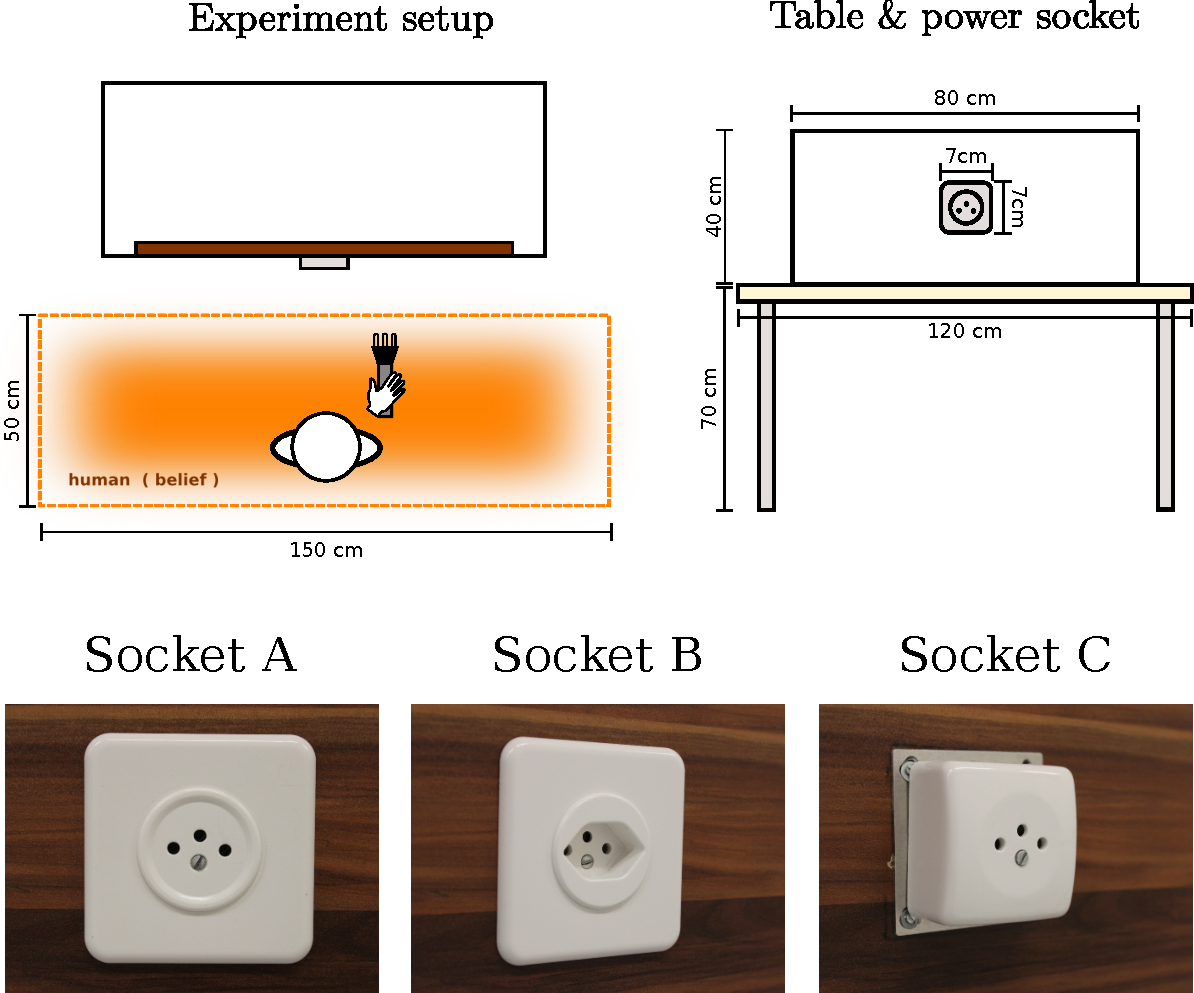
\includegraphics[width=0.8\textwidth]{./ch4-PiH/Figures/Fig/experiment_setup_and_design.pdf}
 \caption{The experimental setup. \textit{Top-left:} A participant (human teacher) is blindfolded and 
    placed within the orange rectangular area always facing the wall. \textit{Top-right:} Dimensions of the 
    the wall and socket. \textit{Bottom:} Three different power sockets, only socket A and B are used for data collection, socket
    C is purely used for evaluating the generalisation of the learned policy.}
    \label{fig:search_task_setup}
\end{figure}

The human teacher holds the plug which is attached to a cylindrical handle with 
an ATI 6 axis force torque sensor (Nano25 \footnote{http://www.ati-ia.com/products/ft/sensors.aspx}) 
to provide \textbf{raw} wrench $\phi \in \mathbb{R}^6$ measurements. We define the \textbf{actual} measurement 
to be a function of the raw wrench, $\tilde{y}_t = h(\phi_t)$, which is a binary feature vector. The feature vector encodes whether a contact is present 
and the direction in which it occurs, which is discretized to the four cardinalities.

On top of the cylinder there is a set of markers used by a motion capture system OptiTrack\footnote{http://www.optitrack.com/}
(which has millimeter tracking accuracy), 
see Figure \ref{fig:plug_cylinder}, to measure both linear, $\dot{x} \in \mathbb{R}^3$, and angular 
velocity, $\omega \in \mathbb{R}^3$, at each time step which is recorded at a rate of 100 Hz. The force and torque information 
from the ATI sensor is recorded at the same rate. 

\begin{figure}
 \centering
 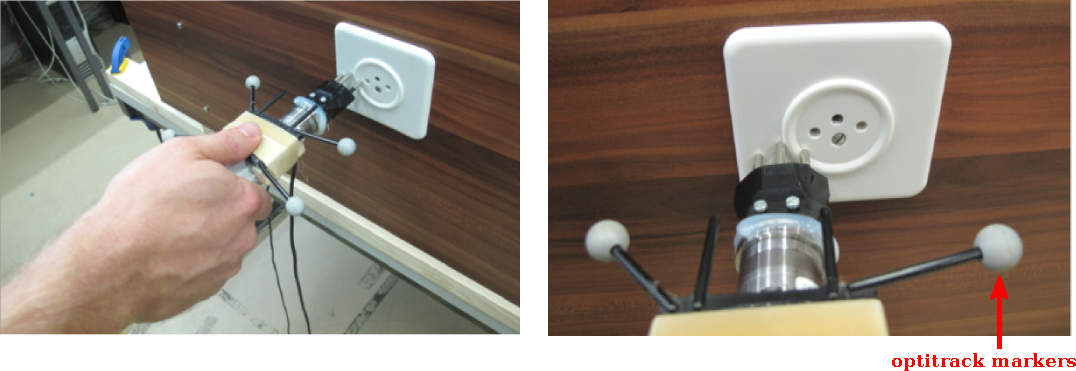
\includegraphics[width=0.8\textwidth]{./ch4-PiH/Figures/Fig/plug_socket_closeup.pdf}
 \caption{Human holding the cylinder plug holder, which is equipped with OptiTrack markers.}
 \label{fig:plug_cylinder}
\end{figure}

In this task, the human's location belief is represented by a probability distribution function. 
The participants' (teachers) initial belief is assumed to be uniformly distributed as depicted 
in orange area of Figure \ref{fig:search_task_setup} and that all subsequent beliefs can be inferred from the measured velocity 
and measurements provided by the ATI and OptiTrack sensors. The following section describes how the belief can be represented, 
computed and compressed.

\subsubsection{Belief state}
%\subsubsection{Belief probability density function}
% Before explaining the measurement model we detail what measurement $\tilde{y}_t$ is.
%This step essentially consists of applying a convolution kernel to the PMF where the covariance 
%is proportional to the measured velocity.
For the task at hand, the belief probability density function,  $p(x_t|y_{0:t},\dot{x}_{0:t})$,  
is a Point Mass Filter (PMF) \cite[p.87]{Bergman99recursivebayesian}, which is a  Bayesian filter.
It is parametrised by a set of grid cells containing valid probabilities 
and is recursively updated by the application of a \textbf{motion}, $p(x_t|x_{t-1},\dot{x}_t)$ 
and \textbf{measurement}, $p(y_t|x_t)$ model. The motion model updates the position of the probability density function 
and subsequently increases the uncertainty of the position.  The measurement model indicates areas 
of the state space from which a measurement $\tilde{y}_t$ could have originated. 
In Figure \ref{fig:PMF} (\textit{Bottom-right}) we illustrate the likelihood when an edge is sensed.

A PMF is chosen to represent the believed location of the plug as the sensing 
the sensing likelihoods are non-gaussian and lead to multi-modal distributions.  
A PMF is able to capture such non-gaussianity whilst remaining fully deterministic 
(which is not the case for a particle filter).

\begin{figure*}
 \centering
   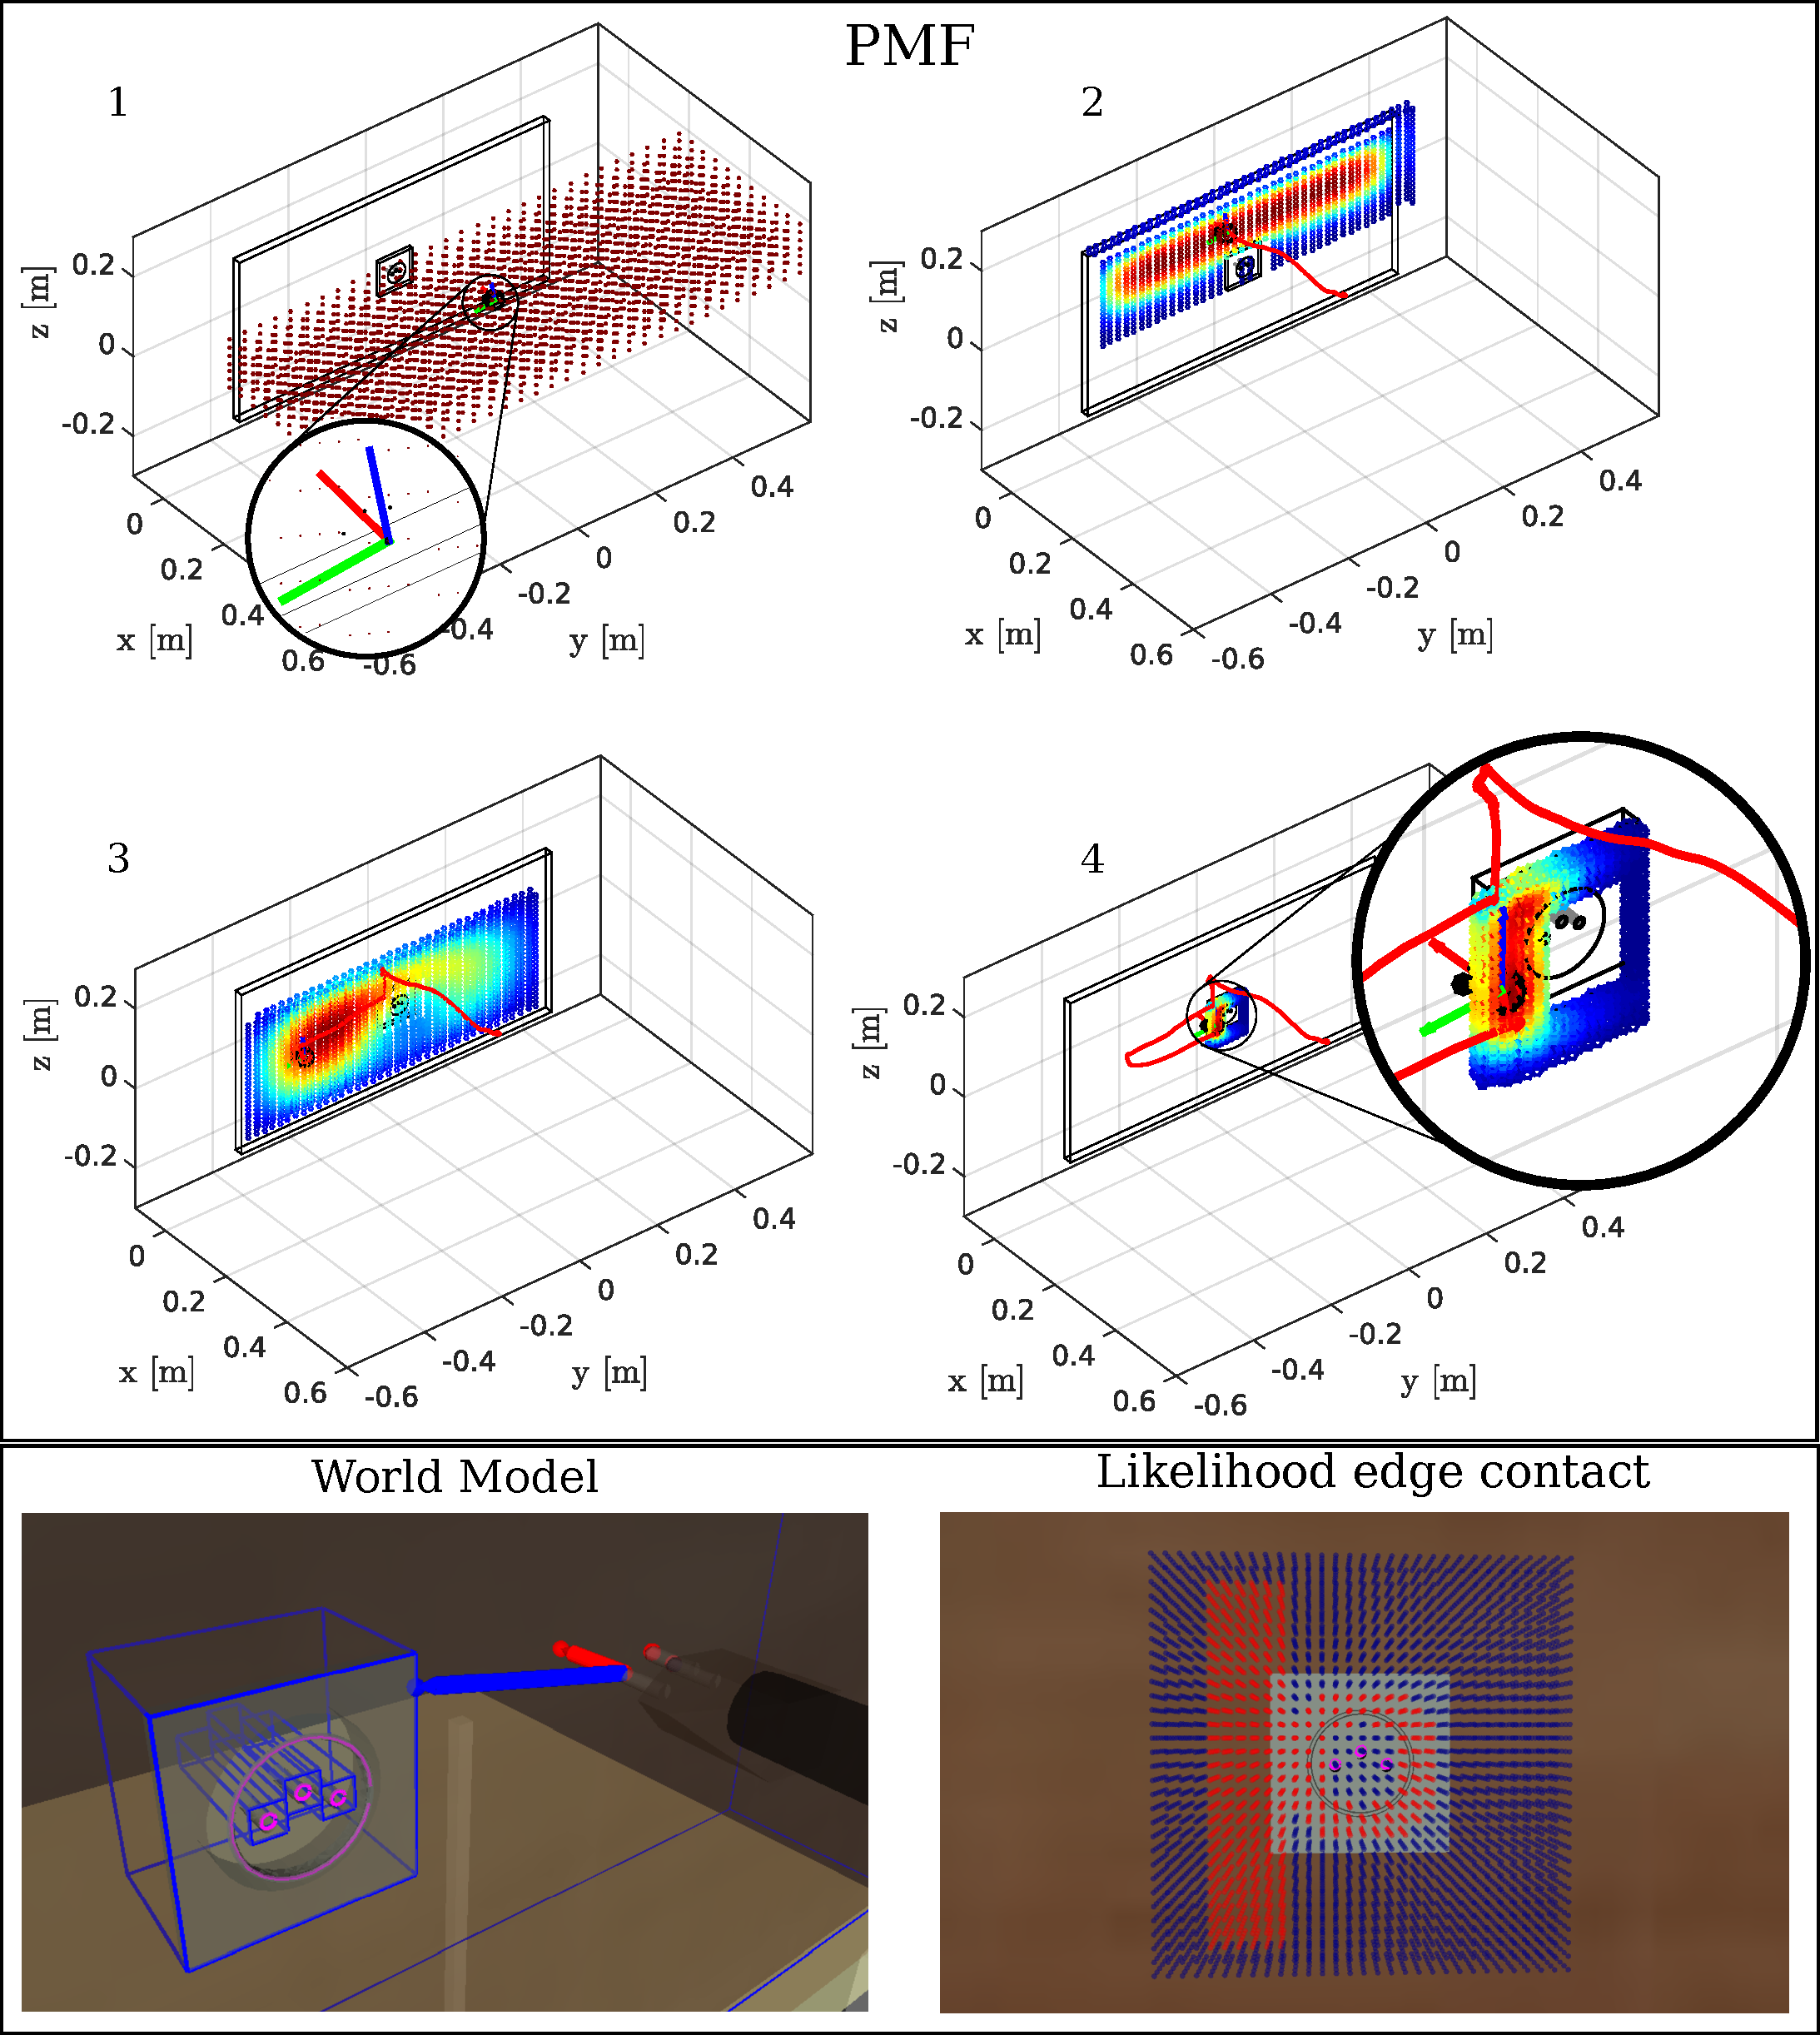
\includegraphics[width=\textwidth]{./ch4-PiH/Figures/PMF/pmf_likelihood_v2.pdf}
   \caption{\textit{Left:} Point Mass Filter (PMF) update of a particular human demonstration. (1) Initial uniform distribution spread over the starting 
   region. Each grid cell represents a hypothetical position of the plug. The orientation is assumed to be known. (2) First contact, the distribution 
   is spread across the surface of the wall. The red trace is the trajectory history. (3) motion noise increases the uncertainty. (4) The plug is in contact with a socket edge.
   \textit{Right}: \textbf{World model}: The plug is modelled by its three plug tips and the wall and sockets are fitted with bounding boxes.
   \textbf{Likelihood}: The plug enters in contact with the left edge of the socket. As a result, the value of the likelihood in all the regions, $x_t$, close the left edge take 
   a value of one (red points)  whilst the others have a value zero (blue points) and areas around the socket's central 
   ring have a value of one. }
  \label{fig:PMF}
\end{figure*}

The probability density function $p(x_t|y_{0:t},\dot{x}_{0:t})$ is high dimensional and thus it is 
impractical to directly learn a statistical policy $\pi_{\theta} : p(x_t|y_{0:t},\dot{x}_{0:t}) \rightarrow \dot{x}_t$
without some form of compression. One possibility would be E-PCA \cite{NIPS2002_2319} which extracts a set of 
representative basis functions which are aslo probability distributions. Although elegant this method 
requires a discretisation of the belief space which is computationally expensive. Instead we choose to 
compress the pdf to a belief space vector composed of the maximum a posteriori, $\hat{x}^{\mathrm{MAP}}_t = \argmax_{x_t} p(x_t|y_{0:t},\dot{x}_{0:t}) \in \mathbb{R}^3$, and the differentiation entropy, 
$U = H\{p(x_t|y_{0:t},\dot{x}_{0:t})\} \in \mathbb{R}$. All pdfs in our recorded data set $D$ are transformed to 
a belief space feature vector, $b_t = [\hat{x}^{\mathrm{MAP}}_t,U]^{\mathrm{T}}$. 

Each participant's demonstration results in a dataset $D=\{\dot{x}^{[i]}_{1:T},\omega^{[i]}_{1:T},\phi^{[i]}_{1:T},b^{[i]}_{1:T}\}$, 
where the upper index $[i]$ references the ith search trajectory (also one execution of the task or one episode) and 
subscript $1:T$ denotes the time steps during the trajectory from initialisation $t=1$ until the end $t=T$. 
%The data consisted of the plug's linear velocity, $\dot{x} \in \mathbb{R}^3$, 
%angular velocity $\omega \in \mathbb{R}^3$, the sensed wrench $\phi \in \mathbb{R}^6$ (force-torque),
%and the belief state, $b$, over the plug's location.

\subsection{Participants and experiment protocol}

To perform the PiH search tasks we recruited 10 student volunteers to be teachers (all male Master's and PhD students).
The participants were aged between 24 and 30 with an average age of 26 years and a standard deviation of 2.4 years.
Each participant carried out 30 demonstrations of the PiH search-task and each session lasted approximately 50 minutes and 
never exceeded one hour. The 10 participants were divided equally in two groups, A and B. Each member of group A began 
by performing 15 PiH searches with socket A, followed by a 10 minute break, finishing with an additional 15 searches with socket B. 
The members of group B performed the same protocol starting with socket B and ending with socket A.
%The group of 5 teachers starting with socket A, will be called ``Group A'' and vis versa, the group of 5 teachers starting with socket B will 
%be referred to as ``Group B''. 
Figure \ref{fig:experiment_design} summarises a walk through of the experiment.
The only exclusion criteria was the inability of the subject to accomplish the task. All participants gave written consent 
for taking part in this study.

%Below we describe the generic experiment taken for the two Groups A \& B of 5 subjects.
The next section describes in detail the protocol for the search task:

\begin{enumerate}
 \item Participant signs a form of consent before starting the experiment.
 \item Each participant is given the opportunity to familiarise himself with the environment and become 
 comfortable in wearing the sensor deprivation apparatus.
 During this time the participant is allowed to practice connecting the plug to the socket whilst standing within its vicinity.  
 \item Once the participant feels sufficiently ready to carry out the task to the best of his ability, the experimenter 
  proceeds to disorient him through the usage of swivel chair. The disorientation process takes 30 seconds and includes
  both translation and rotation motions. After disorientation, the participant is signalled to stand up. The participant
  is reminded that he is facing the direction of the wall and that his starting location is within the orange 
  rectangular area demarcated on the floor. He is then signalled by a light touch to the shoulder 
  that he can start the task.
  \item At task completion, the subject is once again disoriented and the process is repeated a total of 15 times.
  After 15 trials, the subject is given a 10 minute break whilst the experimenter changes the type of socket (A or B). 
  A participant of group A will now continue with socket B. Similarly a participant of group B will continue after the break 
  with socket A.
\end{enumerate}

Each participant carried out a total of 30 PiH-search experiments, giving a total of 300 demonstrations.

\begin{figure}
\centering
 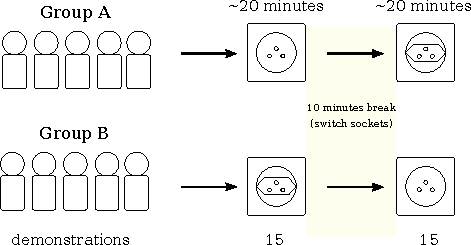
\includegraphics[width=0.8\textwidth]{./ch4-PiH/Figures/Fig/experiment_design_v2.pdf}
 \caption{Experiment protocol. The participants are divided in two groups of 5, Group A begins with socket A 
 and after a short break repeats the task with socket B. The same logic holds for Group B.
 For each socket 15 executions of the task are recorded.}
 \label{fig:experiment_design}
\end{figure}

%the usage of a chair as mentioned previously. The teachers were reminded that they were facing the direction of 
%the fake wall and that the starting location would be always within the orange rectangular area. 


\paragraph{Preliminary results}

Both groups A and B took $9\pm10$s to find the socket's edge, regardless of the socket type. This is to be expected since the sockets 
are at the same location. It took a further $8\pm7$s on average for group B to connect
socket B and $12\pm10$s on average for group A to connect socket A. As we can see this is not a straight forward task when considering
the sensory deprivation. See Figure \ref{fig:experiment_setup_data} (\textit{Bottom}) for the time taken to connect the plug to the socket.
In Appendix \ref{app:anova_socket} we report the results of a non-parametric statistical analysis on the time taken to connect
the sockets and we find that it takes 4 seconds more to connect socket A than socket B. This is somewhat expected as 
socket B has a funnel which can help to contain the subject to within the vicinity of the holes.

As connecting to socket A is more difficult we will \textbf{using only these demonstrations} as training data to learn a policy. Both
socket B and C will be used solely to evaluate the generalisation of the policy.

\begin{figure}
 \centering
   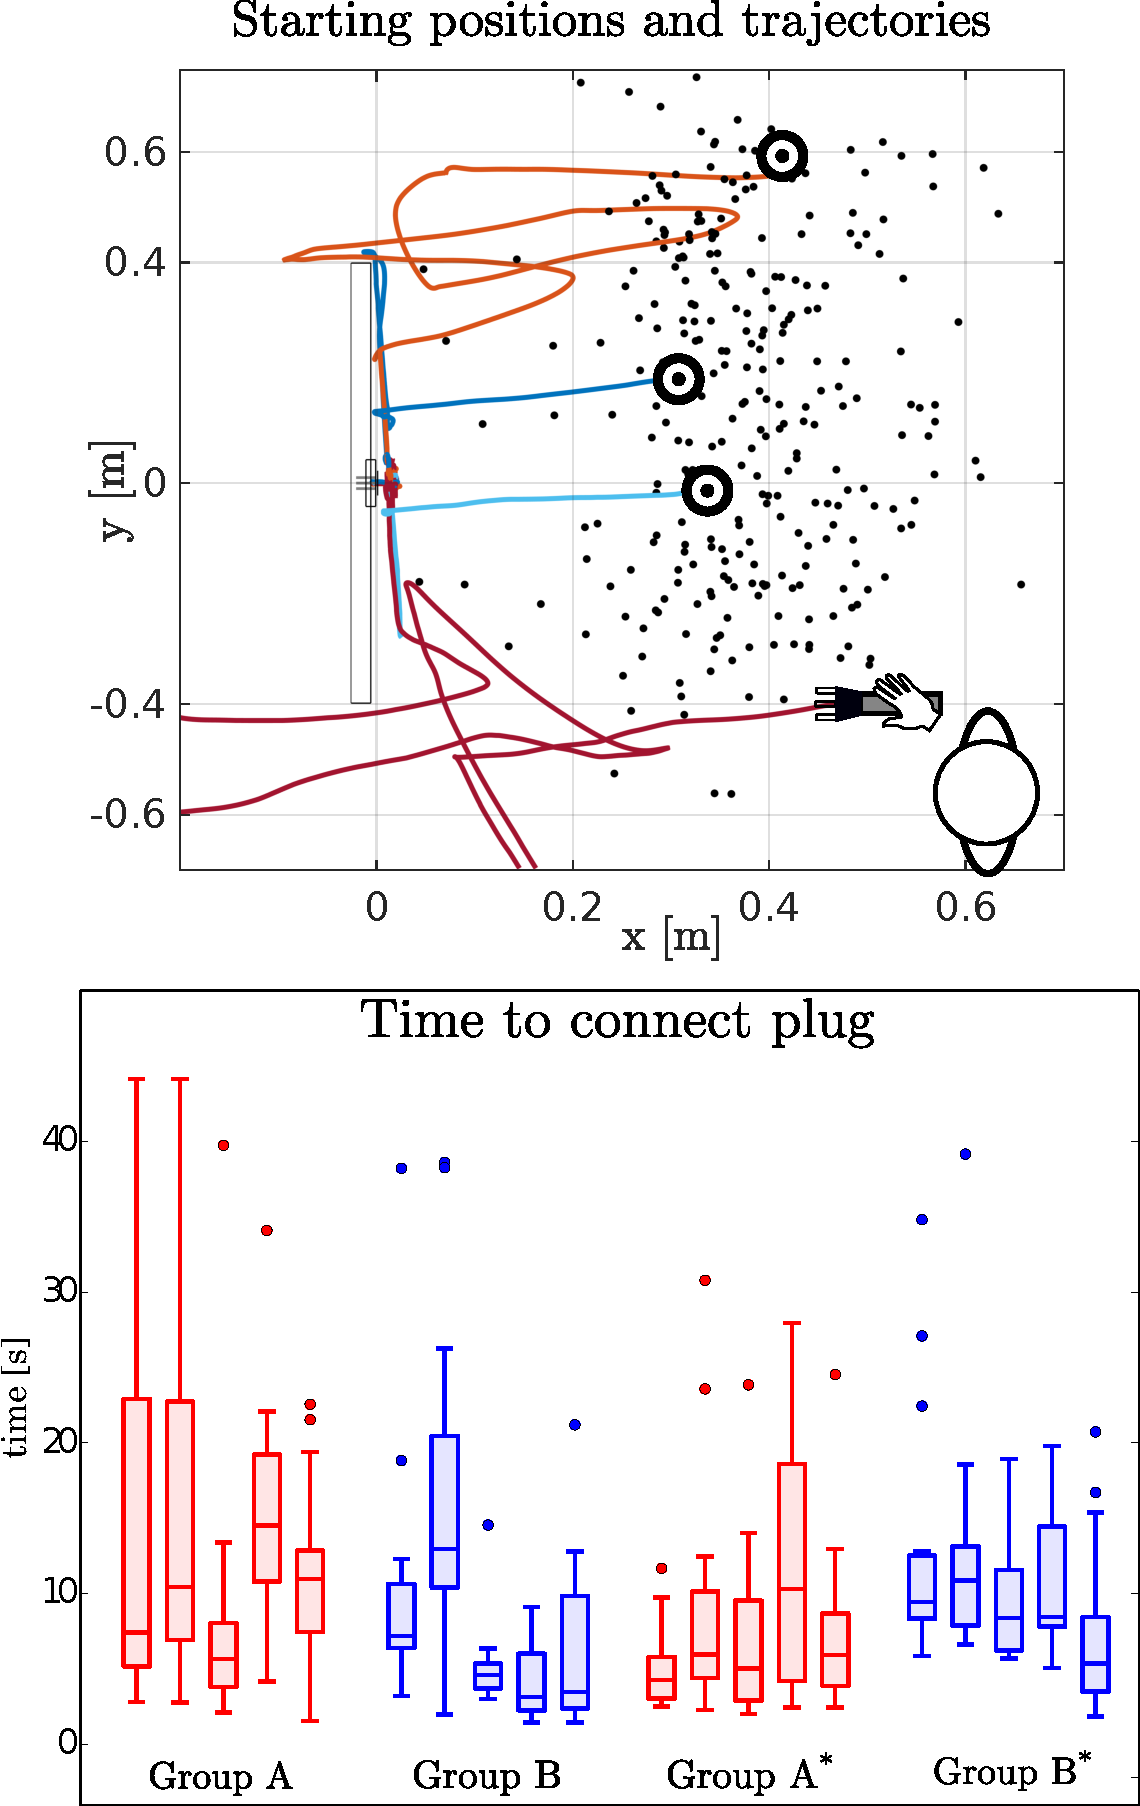
\includegraphics[width=\textwidth]{./ch4-PiH/Figures/Fig/start_position_v2.pdf}
   \caption{\textit{Top}: Black points represent the starting position of the end-effector
   for all the demonstrations. Four trajectories are illustrated. \textit{Bottom:} 
   Time taken for the teachers to accomplish the PiH once the socket is localised. Group A and B are depicted in red 
   and blue. The second later indicates which socket is used, see Figure \ref{fig:experiment_design}.}
   
   %The asterisk indicates that the group has changed sockets, so Group A\textsuperscript{*} means
   %that Group A is now performing the task with socket B and Group B\textsuperscript{*} means that group B is now performing 
   %the task with socket A.}
  \label{fig:experiment_setup_data}
\end{figure}

%In Figure \ref{fig:experiment_setup_data} we can see the time taken by the teachers to accomplish the task. 
%A group of 10 human teachers participated in the plug-socket experiment. Each teacher performed the search and PiH 
%for sockets A and B. A teacher of group A (starting with socket A), would start by performing 15 times the search and connection 
%with socket A and after a short break, during which socket A was replaced by socket B, would carry on to perform 15 trials 
%with socket B.

%The location belief of the humans was represented by a probability density function. We made the assumption 
%that after the disorientation step the human's believed location would be uniform and spread across the 
%rectangular starting area. Although the mental state of the human remains 
%unobservable, there is sufficient evidence to support our assumption that his belief state
%gets updated in a Bayesian fashion [citation].

\section{Learning Actor and Critic}\label{ch4:learning-value-actor}

In our approach we learn two data driven policies. The first policy maps from belief space 
to linear velocity $\pi_{\Param_1} : b_t \mapsto \dot{x}_t$ and the second from 
angular sensed wrench to angular velocity, $ \pi_{\Param_2} : \phi_t \mapsto \omega_t$.
We chose to learn the belief policy $\pi_{\Param_1}$ in a Actor-Critic RL framework 
and the wrench policy $\pi_{\Param_2}$ directly from the demonstrated data as was done 
in \cite[Chap. 5]{Kronander2015}, which proved to be efficient in overcoming jamming during the PiH. 
A POMDP solver's objective is to find a policy (Actor), $\pi_{\Param_1}: b \mapsto u$, which maximises 
the value function (Critic) $V^{\pi_{\Param_1}} : b \mapsto \mathbb{R}$ for an initial belief, $b_{0}$. The value function
is the expected reward over an infinite time horizon.
\begin{equation}\label{eq:value_function}
  V^{\pi_{\Param_1}}(b_t) = \mathbb{E}\Bigg\{ \sum_{t=0}^{\infty} \gamma^{t} r_{t+1} | b_0=b,\pi_{\Param_1}\Bigg\}
\end{equation}

In an Actor-Critic setting, the temporal difference error, $\delta_t \in \mathbb{R}$, of the value function (the Critic) is 
used as a learning signal to update simultaneously itself and the actor (the policy). In our method, 
two separate policies are learned, one for the linear velocity and the other for the angular velocity.
The orientation is kept constant until the start of the connection of the plug to the socket.
The angular velocity policy used and learned only during the insertion of the plug to the socket where it is necessary
to control the orientation to avoid jamming.

\subsection{Actor \& Critic}
%Two control policies are learned; The first $\pi_{\Param_1}: b \mapsto \U$, maps belief state $b$ to linear velocity, 
%$\U$ and the second, $\pi_{\Param_2}: \phi \mapsto \omega$ , sensed wrench, $\phi$, to angular velocity, $\omega$.
%These actors/policies are parametrised by a Gaussian Mixture Model (GMM), Equation \ref{eq:GMM}.
Both the linear and angular velocity policies are parameterised by a Gaussian Mixture Model (GMM), Equation \ref{eq:GMM}.

\begin{equation}
 \pi_{\Param}(\U,\B) = \sum\limits_{k=1}^{K} \piK \, g(\U,\B;\MuK,\SigK) \label{eq:GMM}
\end{equation}
The parameters $\Param = \{w^{[k]},\MuK,\SigK\}_{1,\dots,K}$, are the weights, means and covariances 
of the individual Gaussian functions, $g(.)$,
\begin{center}
$\MuK =  \begin{bmatrix} \MuK_{\U} \\ \MuK_{\B} \end{bmatrix}$, 
$\SigK =  \begin{bmatrix} 
	  \SigK_{\U\U} & \SigK_{\U\B} \\
	  \SigK_{\B\U} & \SigK_{\B\B}
	  \end{bmatrix}$
\end{center}
where $\sum_{k} w^{[k]} = 1$, $\MuK_{\U} \in \mathbb{R}^{3}$ and  $\MuK_{\B} \in \mathbb{R}^{4}$.
%There are three steps to learning and use for control a GMM model.  Firstly a generative model is learned through 
%Expectation-Maximisation (EM) which maximised the likelihood

A generative model of the angular velocity and wrench $\pi_{\Param_2}(\omega,\theta)$ and a generative model 
of the linear velocity and belief state $\pi_{\Param_1}(\dot{x},b)$ are learned. 
In both cases we use the Bayesian Information Criterion to determine the number of Gaussian functions.
In the next section, we will show how the parameters of $\pi_{\Param_1}$ can be adapted by the value function of the Critic.

%First a generative model, $p_{\Param}(\dot{x},b)$, is learned through maximising the likelihood of 
%the dataset by Expectation-Maximisation (EM). 
%Second the conditional is taken $p_{\Param}(\dot{x}|b)$
%giving a distribution over the applicable actions $\dot{x}$, Equation \ref{eq:GMC}

%\begin{equation} 
%  \pi_{\Param}(\U|\B) = \sum\limits_{k=1}^{K} \piK(\B) \cdot  g(\B;\MuK_{\U|\B},\SigK_{\U|\B}) \label{eq:GMC}
%\end{equation}
%\begin{align}
% w^{[k]}(\B)  &= \frac{\piK \cdot g(\B;\MuK_{\B},\SigK_{\B\B})}{\sum_{j=1}^{K} w^{[j]} \cdot g(\B;\Mu{j}_{\B},\Sig{j}_{\B\B}) } \\
% \MuK_{\U|\B}   &= \MuK_{\U} + \SigK_{\U\B} \invSigK_{\B\B}(\B - \MuK_{\B})\\
%  \SigK_{\U|\B} &= \SigK_{\U\U} - \SigK_{\U\B}\invSigK_{\B\B}\SigK_{\B\U}
%\end{align}
%Thirdly a concrete action, to be applied, is derived from the conditional distribution. One approach is
%to take the expectation of the conditional, $\hat{\U} = \mathbb{E}_{p_{\Param}(\U|\B)}\{\U\}$ whilst 
%another is to draw a sample $\U \sim p_{\Param}(\U|\B)$. 


% Q-learning and TD(0) are based on the dynamic porgramming algorithm known as value iteration.
% 
%\cite{NIPS2008_3501} (Fitted Q-iteration by Advantage Weighted Regression)
%
%We use a combination of function approximation and dynamic programming to learn a value function 
%of the belief state with respect to the given task.

%\cite{Szepesvari:2010}

The Critic (the value function, Eq. \ref{eq:value_function}) evaluates 
the performance of the current policy. It is the expected future reward given the current 
belief state and policy.
In our method a reward of $r=0$ is received at each time step
until the goal (plug-socket connection) is achieved, where a reward of 100 is given, $r_{T}=100$.
Given the continuous nature and dimensionality of the belief space we use Locally Weighted Regression \cite{Atkeson97locallyweighted}
(LWR) as a function approximator of the value function, $V^{\pi}(b)$. LWR is a memory-based non-parametric function 
approximator. It keeps a set of input-target pairs $\{(\B,r)\}$ as parameters. When a value, $\B$, is 
queried, a set of $p$ neighbouring points are chosen from the input space and are 
weighted according to a distance metric. The predicted output is given by a weighted 
least square of the $p$ points. Equation \ref{eq:W} is the distance function used where 
$D$ is a diagonal matrix.

\begin{equation}\label{eq:W}
 W_{i,i}  = \exp\left(-\frac{1}{2}(\B - \B_i)^{\mathrm{T}}\, D^{-1} \, (\B - \B_i) \right)
\end{equation}
A new value is queried according to Equation \ref{eq:lwr_predict},
\begin{equation}\label{eq:lwr_predict}
  V^{\pi}(b) = \B \,(B^{\mathrm{T}} W B)^{-1} B^{\mathrm{T}} W \mathbf{r}
\end{equation}
where $B = (\B_1,\dots,\B_p)^{\mathrm{T}} \in \mathbb{R}^{(D\, \times\, p)}$, $W \in \mathbb{R}^{(p\, \times\, p)}$ is
a diagonal matrix, $\mathbf{r} = (r_1,\cdots,r_p)^{\mathrm{T}} \in \mathbb{R}^{(p\, \times\, 1)}$

%We chose this method because it is a safe regressor to use when estimating a value 
%function \cite{Boyan95generalizationin} and is very flexible since it is non-parameteric.

\subsection{Fitted policy evaluation and improvement}\label{sec:fpe}

\paragraph{Policy evaluation}\\

To learn the value function we make use of batch reinforcement learning \cite{EGW05}, also known as Experience replay.
This is an offline method which applies multiple sweeps of the Bellman backup operator 
over a dataset of tuples $\{(\Bi_t,\Ui_t,r^{[i]}_{t},\Bi_{t+1})\}_{i=1,\cdots,M}$ until the Bellman residual,
$||V^{\pi}_{k+1}(\B) - V^{\pi}_{k}(\B)||$, converges. 

\begin{center}
\begin{minipage}{.65\linewidth}
\begin{algorithm}[H]
\label{alg:fpe}
\SetKwInOut{Input}{input}
\SetKwInOut{Output}{output}
\Input{$\epsilon$, $\{(\B^{[i]}_t,r^{[i]},\B^{[i]}_{t+1})\}_{i=1,\cdots,M}$}
\Output{$\hat{V}^{\pi}_{k}(\B_t)$}
\BlankLine
\While{$||\hat{V}^{\pi}_{k+1}(\B) - \hat{V}^{\pi}_{k}(\B)|| < \epsilon$}{
  $\hat{V}^{\pi}_{k+1}(\B_t)$ = Regress($\B$, $r_t + \gamma \hat{V}^{\pi}_k(\B_{t+1}))$
}
\caption{Fitted Policy Evaluation}
\end{algorithm} 
\end{minipage}
\end{center}
Batch RL methods are used by a broad spectrum of research to learn policies. 
Most of them have focused on learning the Q-value function directly (Fitted Q-Iteration) 
\cite{NIPS2008_3501,EGW05,Riedmiller2005}. Although this solves the control problem it requires discretisation 
of the action space or assumes quantifiable actions, as the 
Q-Bellman backups, $\hat{Q}(\B_t,\U_t) \leftarrow \gamma \max_{\U_{t+1}} \hat{Q}(\U_{t+1},\B_{t+1})$, 
require an optimisation over the action space, $\U_{t+1}$, to find the best applicable action. 
Given the dimensionality and continuity of our problem we opt for an on-policy evaluation method
which requires multiple \textit{policy evaluation} and \textit{policy improvement} iterations to achieve an optimal policy.
In order for the RL-PbD-POMDP and PbD-POMDP to be comparable we will only be performing one iteration of policy evaluation
and improvement, hence Algorithm \ref{alg:fpe} is applied only once to the dataset.
% Need to make clear we only do one iteration

%Which is not the case for Fitted Value Iteration (FVI) and Fitted Q-Iteration (FQI).
%After we applied the fitted policy evaluation to our dataset get the expected future 
%reward for each of the belief belief states, giving us a new dataset:
%$D = \big\{\U^{[i]}_{1:T},\omega^{[i]}_{1:T},\phi^{[i]}_{1:T},\B^{[i]}_{1:T},v^{[i]}_{1:T}\big\}^{i=1\dots N}$, where $v^{[i]}_t = \hat{V}^{\pi}(\Bi_t)$.
\paragraph{Policy improvement}\\
%\subsection{Policy improvement}

The Temporal Difference (TD) error $\delta^{\pi}_t = r_{t+1} + \gamma V^{\pi}(b_{t+1}) - V^{\pi}(b_t)$ 
given by the critic is used to update the actor  \cite[Chap. 6]{sutton1998reinforcement}. 
In our offline approach the value function of the belief state, $\hat{V}^{\pi}(\B)$, is estimated 
until convergence and then used to update the actor. This offline batch 
method has the advantage that no divergence can occur during the learning process.

We update the Actor policy given the Critic value function through a modification of the Maximisation step in  Expectation-Maximisation (EM) 
for Gaussian Mixture Models. We refer to this modification as Q-EM which is strongly related to a Monte-Carlo EM-based policy 
search approach \cite[p.50]{p_search_surv_2011}. 

The reward of a demonstrated trajectory (one episode) is given by the discounted return, Equation $\ref{eq:disc_return}$,
\begin{equation}\label{eq:disc_return}
 R(\B^{[i]},\U^{[i]}) = \sum_{t=0}^{\mathrm{T^{[i]}}} \gamma^t \, r(\B^{[i]}_t,\U^{[i]}_t)
\end{equation}
where the index $i$ stands for the $i$th episode.
All policy gradient approaches seek to find a set of parameters, $\Param$, of the Actor,
which will maximise the expected reward, equivalent to maximising Equation \ref{eq:expected_reward},
\begin{align}\label{eq:expected_reward}
 J(\Param) &= \mathbb{E}_{p_{\Param}}\{R\} \nonumber \\
	  &= \sum\limits_{i=1}^{N}   \underbrace{\left( \prod_{t=0}^{T^{[i]}} \pi_{\Param}(\U^{[i]}_t,\B^{[i]}_t) \right)}_{p_{\Param}(\tau_i)} \, R(\tau_i) 
\end{align}
where $\tau_i = \{(\U_0,\B_0),\cdots,(\U_T^{[i]},\B_T^{[i]}) \}$ are the state-action samples of the $i$th episode.
To find the parameters which maximise the cost function, $\argmax_{\Param} J(\Param)$, its derivative is set to zero. 
As this cannot be done directly, we maximise the logarithmic lower bound of the cost function which results in 
Equation \ref{eq:grad_log_cost}, see Appendix \ref{app:lb} for the derivation.

\begin{equation} \label{eq:grad_log_cost}
  \nabla_{\Param}\mathcal{Q}(\Param,\Param') = \sum\limits_{i=1}^{N} \sum\limits_{t=0}^{T^{[i]}} \nabla_{\Param}\log \pi_{\Param}(\U^{[i]}_t,\B^{[i]}_t) \, Q^{\pi_{\Param'}}(\U^{[i]}_t,\B^{[i]}_t)
\end{equation}

Setting the derivative of Equation \ref{eq:grad_log_cost} to zero and solving for the parameters
$\Param=\{w,\boldsymbol{\mu},\boldsymbol{\Sigma}\}$ leads to a Maximisation update step of EM
which is weighted by $Q^{\pi_{\Param'}}$.
We use the Critic's TD error as a substitute for $Q^{\pi}$. Assuming that our estimated value function, $\hat{V}^{\pi}$, 
is close to the true value function $V^{\pi}$, the TD error $\delta^{\pi}$ is an unbiased estimate of the advantage function, Equation \ref{eq:advantage_f} 
(see Appendix \ref{app:unbiased_delta}).
\begin{equation}\label{eq:advantage_f}
 A^{\pi}(\U_t,\B_t) =  Q^{\pi}(\U_t,\B_t) - V^{\pi}(\B_t) = \delta^{\pi}_t
\end{equation}
Using the advantage function as means of policy search is popular with methods such as
Natural Actor Critic (NAC) \cite{peter_nac_2008}.

Each state-action sample $j$ has an associated weight, $\delta_j \in \mathbb{R}$, where $\delta_j > 0$ means that the 
$j$th state action-pair lead to an increase in the value function and $\delta_j < 0$ lead to 
a decrease in the value function. The data log-likelihood is re-weighted accordingly, giving more importance to data points which lead to a gain. Since 
the Q-EM update steps cannot allow negative weights, the TD error is rescaled to be between 0 and 1. % we already sed this

The reader is referred to Appendix \ref{app:grad} for the Maximisation update step of Q-EM for a 
GMM parameterization of the policy.

%We learn the plug-socket search policy using the Q-EM update rules for a GMM parametrisation with the 
%data set, $D_1 = \big\{\U^{[i]}_{1:T},\B^{[i]}_{1:T},\delta^{[i]}_{1:T}\}^{i=1\dots N}$ and learn a second policy for inserting the 
%final steps of connecting the plug to socket with data set $D_2 = \{\omega^{[i]}_{1:T},\phi^{[i]}_{1:T}\}^{i=1\dots N}$. 
%In Figure \ref{fig:data_flow} we illustrate the data flow and the policies which are learned. Note that we also learn a belief space 
%policy directly from the demonstrations, $\pi_{\Param_3}(\U,\B)$, which we will refer to as the GMM policy and we will use it to compare 
%with the policy corrected by the Critic, which we call the Q-EM policy.
%\begin{figure}[h]
%  \centering
%  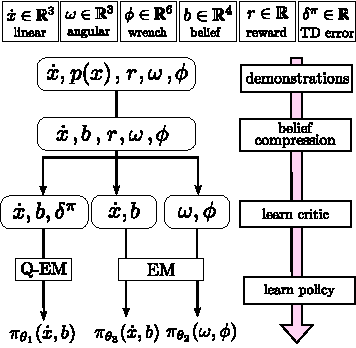
\includegraphics{Figures/data_flow_2.pdf}
%  \caption{Data flow and policies learned. The original data consists of five variables which are recorded during the demonstrations given 
%  by the human teachers. The probability density function of the believed location of the end effector is compressed to a belief state, which 
%  is the most likely state and entropy. The value function is learned via fitted policy iteration and each data point has a temporal difference 
%  error. An actor policy is learned via Q-EM, $\pi_{\Param_1}(\U,\B)$ , a regular policy is learned via the standard EM approach, $\pi_{\Param_3}(\U,\B)$
%  and a plug insertion policy is learned $\pi_{\Param_2}(\U,\B)$.}
%  \label{fig:data_flow}
%\end{figure}


%\subsection{Fitted policy evaluation and improvement}
\paragraph{2D example fitted policy evaluation and improvement}\\

To illustrate the mechanism of fitted policy evaluation and improvement, we give a 2D example 
of its application, see Figure \ref{fig:fpe_example}. The \textit{Top-left} subfigure
depicts 10 trajectories demonstrated by two teachers going from start (white circle) to goal (orange star) state. 
The optimal path is a straight line passing in between two obstacles. 
Neither teacher demonstrated the optimal straight path. 

In the \textit{Bottom-left}, a GMM is fitted $\pi_{\Param}(\U,\X)$ to the teachers' data, using the standard EM-algorithm.
Taking the policy to be the output of Gaussian Mixture Regression (GMR) $\mathbb{E}\{\pi_{\Param}(\U|\B)\}$ we obtain different
behaviours than those demonstrated by the human teachers. The GMR averages the different modes encoded by the Gaussian functions 
which results in a mixing of the original demonstrated behaviours. No trajectories of the GMR policy truly replicate 
the demonstrated behaviour. 

In the \textit{Top-right} subfigure, we apply fitted policy evaluation to the original demonstrated data (discount 
factor $\gamma=0.99$ and reward $r=1$ when the goal is reached and zero otherwise) and compute the value function.

The \textit{Bottom-right} subfigure illustrates the GMM policy learned with the Q-EM algorithm. As 
the advantage function $ A^{\pi}(\X,\U)$ is highest along the start-goal axis, data points
following this gradient will have a higher weight. This results in a policy with better 
rollouts (closer to the optimal path) than the trajectories generated by the policy learned via standard EM. 
%The \textit{Bottom-right} subfigure illustrates of 
%the Q-EM policy and rollout trajectories.

\begin{figure}
 \centering
 \setlength\fboxsep{0pt}
  \setlength\fboxrule{0.25pt}
  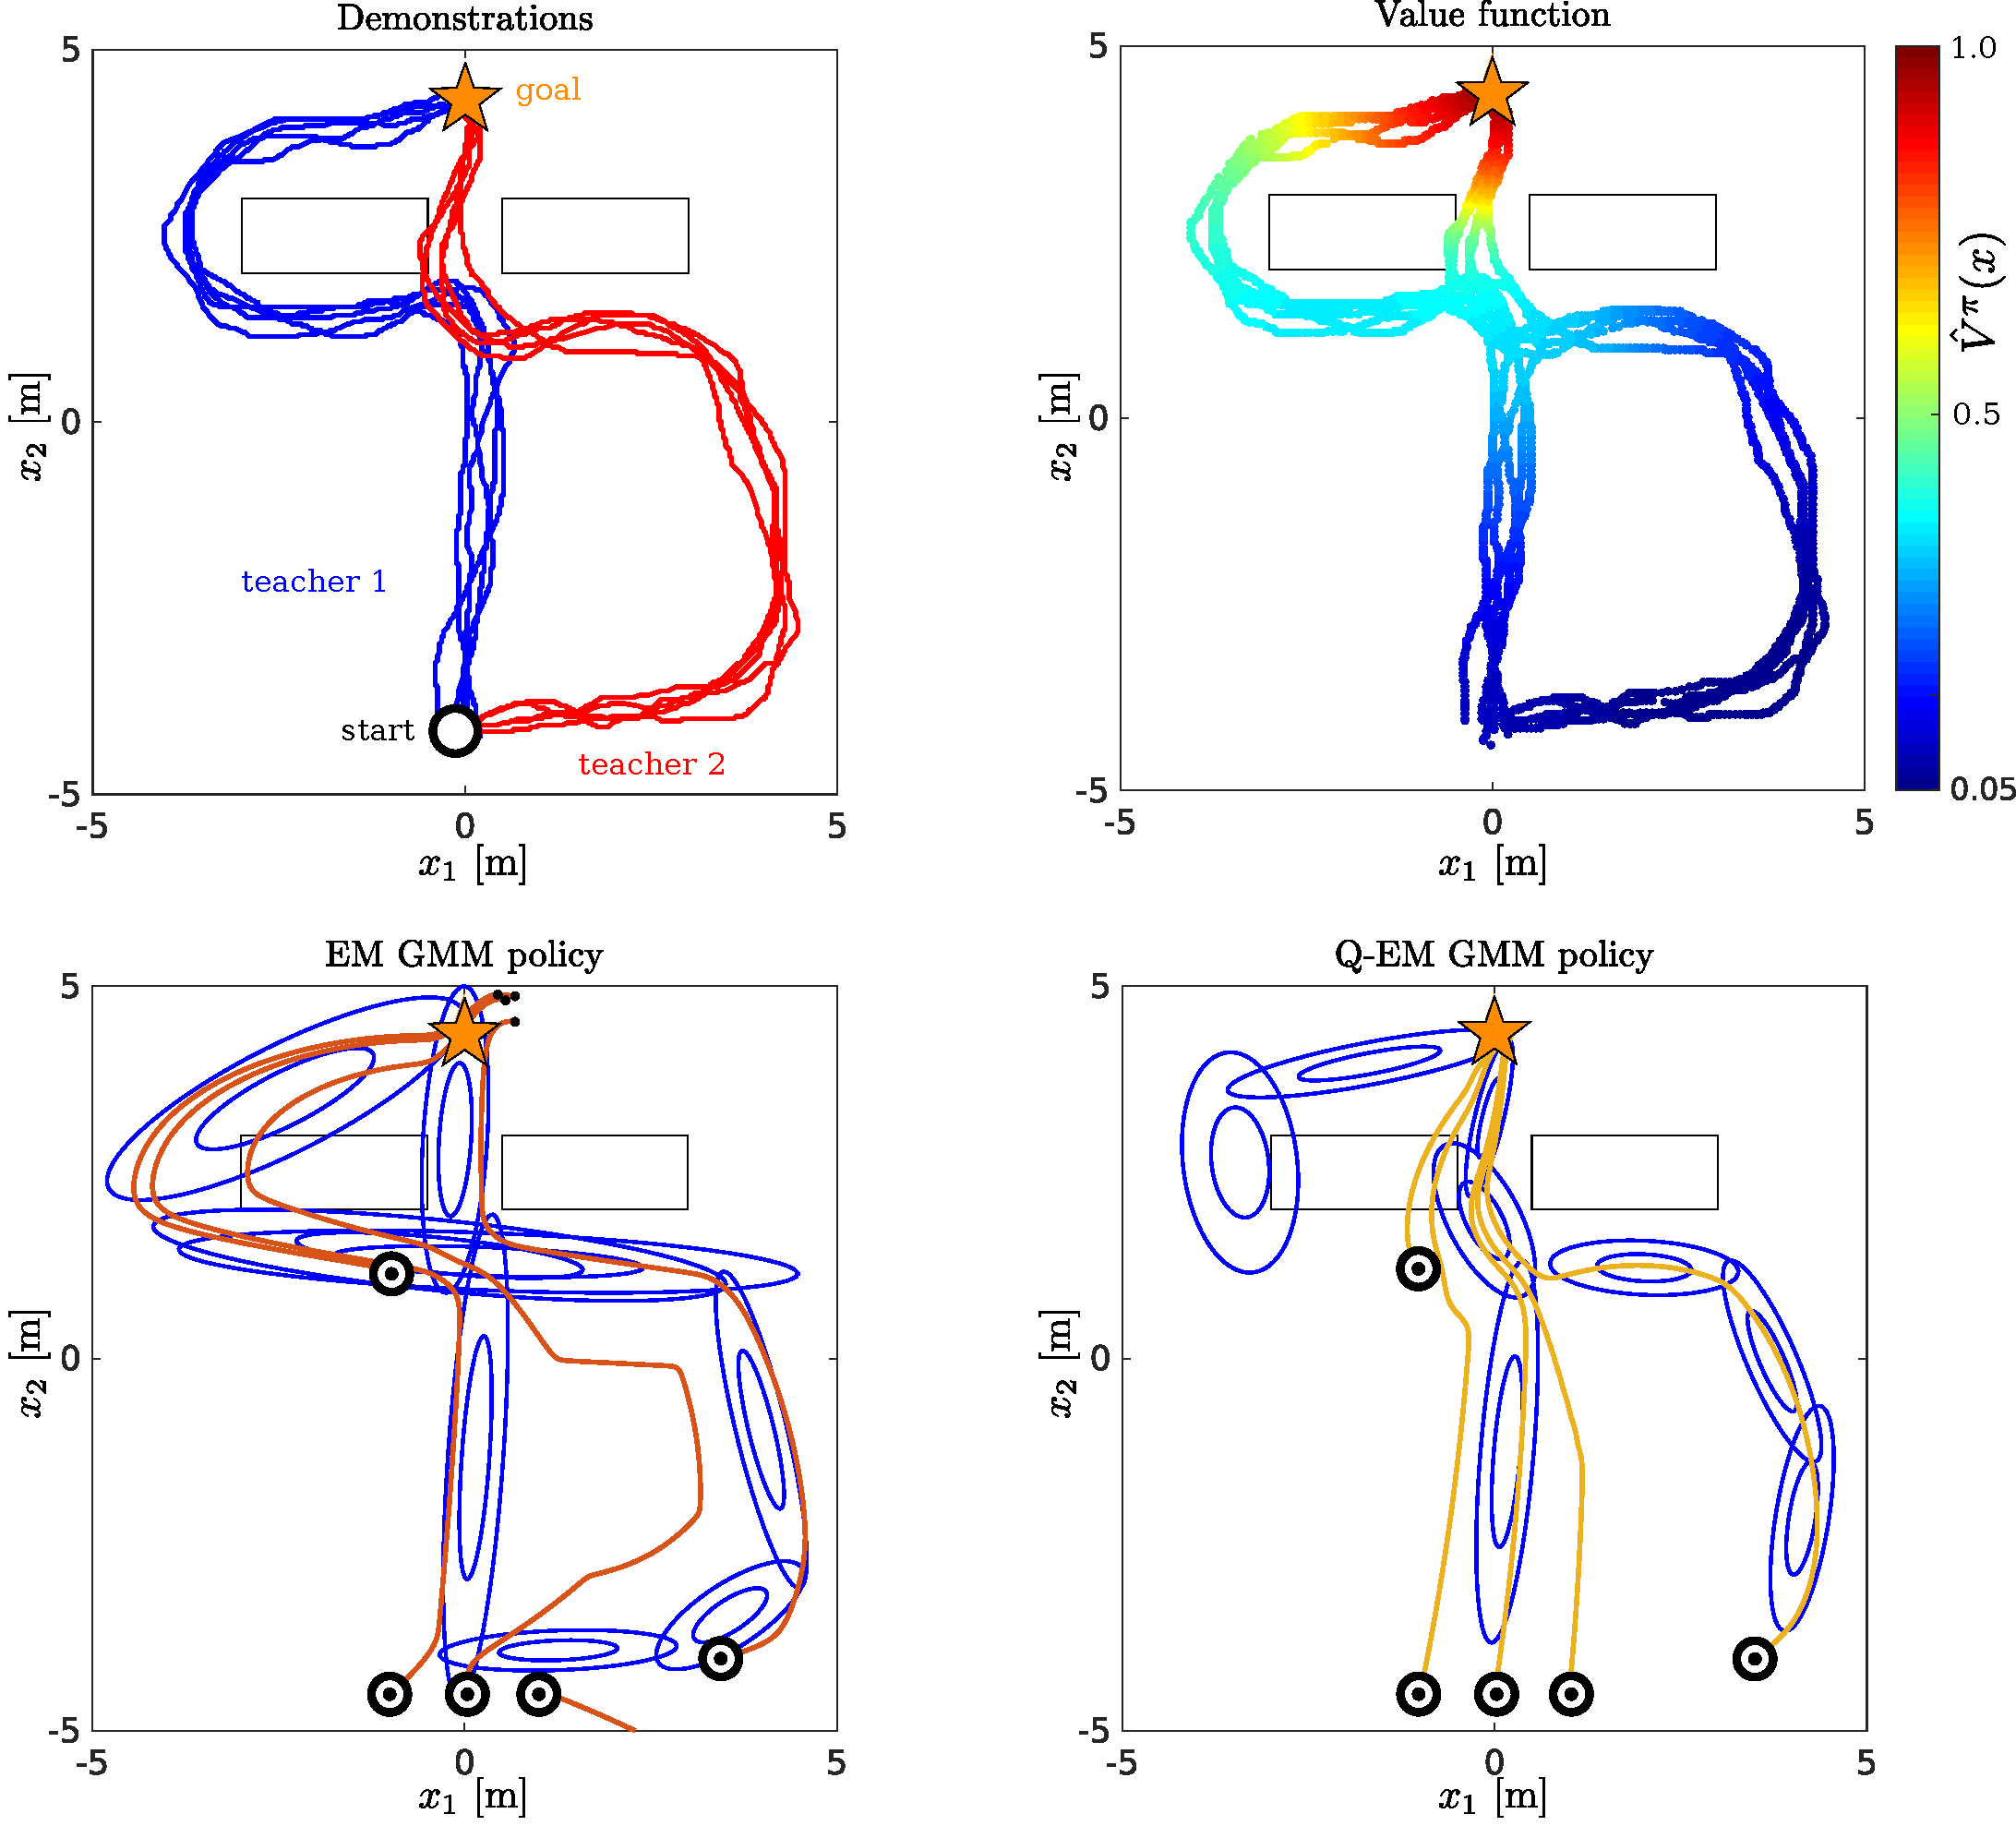
\includegraphics[width=\textwidth]{./ch4-PiH/Figures/fpe_example.pdf}
 \caption{Fitted policy evaluation \& improvement example. 
  \textit{Top-left:} The goal of the task is to reach the goal state. The first teacher (blue) demonstrates 
  five trajectories which contours the obstacle in front of the goal. The second teacher (red) demonstrates 
  5 trajectories which initially deviate from the goal before passing between the two obstacles. 
  \textit{Bottom-left:} The EM algorithm is used to fit a GMM to the teachers' original data. 
  The marginal $\pi_{\Param}(\X)$ is plotted in blue and trajectories generated by the 
  policy $\mathbb{E}\{\pi_{\Param}(\U|\X)\}$ in orange. \textit{Top-right} \textit{Policy Evaluation:}.  
  Value function after fitted policy evaluation terminated, the reward function 
  is binary, $r=1$ at the goal and zero otherwise, and a discount factor $\gamma = 0.99$ is used.
  \textit{Bottom-right} \textit{Policy Improvement:} the GMM is learned with the Q-EM algorithm in which 
  each data point's weight proportional to the advantage function.
 }
  \label{fig:fpe_example}
\end{figure}

\paragraph{Belief state fitted policy evaluation}

Returning to the PiH-search task with socket A, the Fitted Policy Evaluation (FPE) Algorithm \ref{alg:fpe} is applied to the 
demonstrations. In Figure \ref{fig:ch4:Figure1}  we illustrate the value function of the most likely state after the FPE algorithm converges. 
As expected, the value function is high closest to the socket and around the axis $z=0$ and $y=0$. 
When policy improvement via Q-EM is applied the Gaussian functions of the GMM will favour these locations. 

\begin{figure}
 \centering
 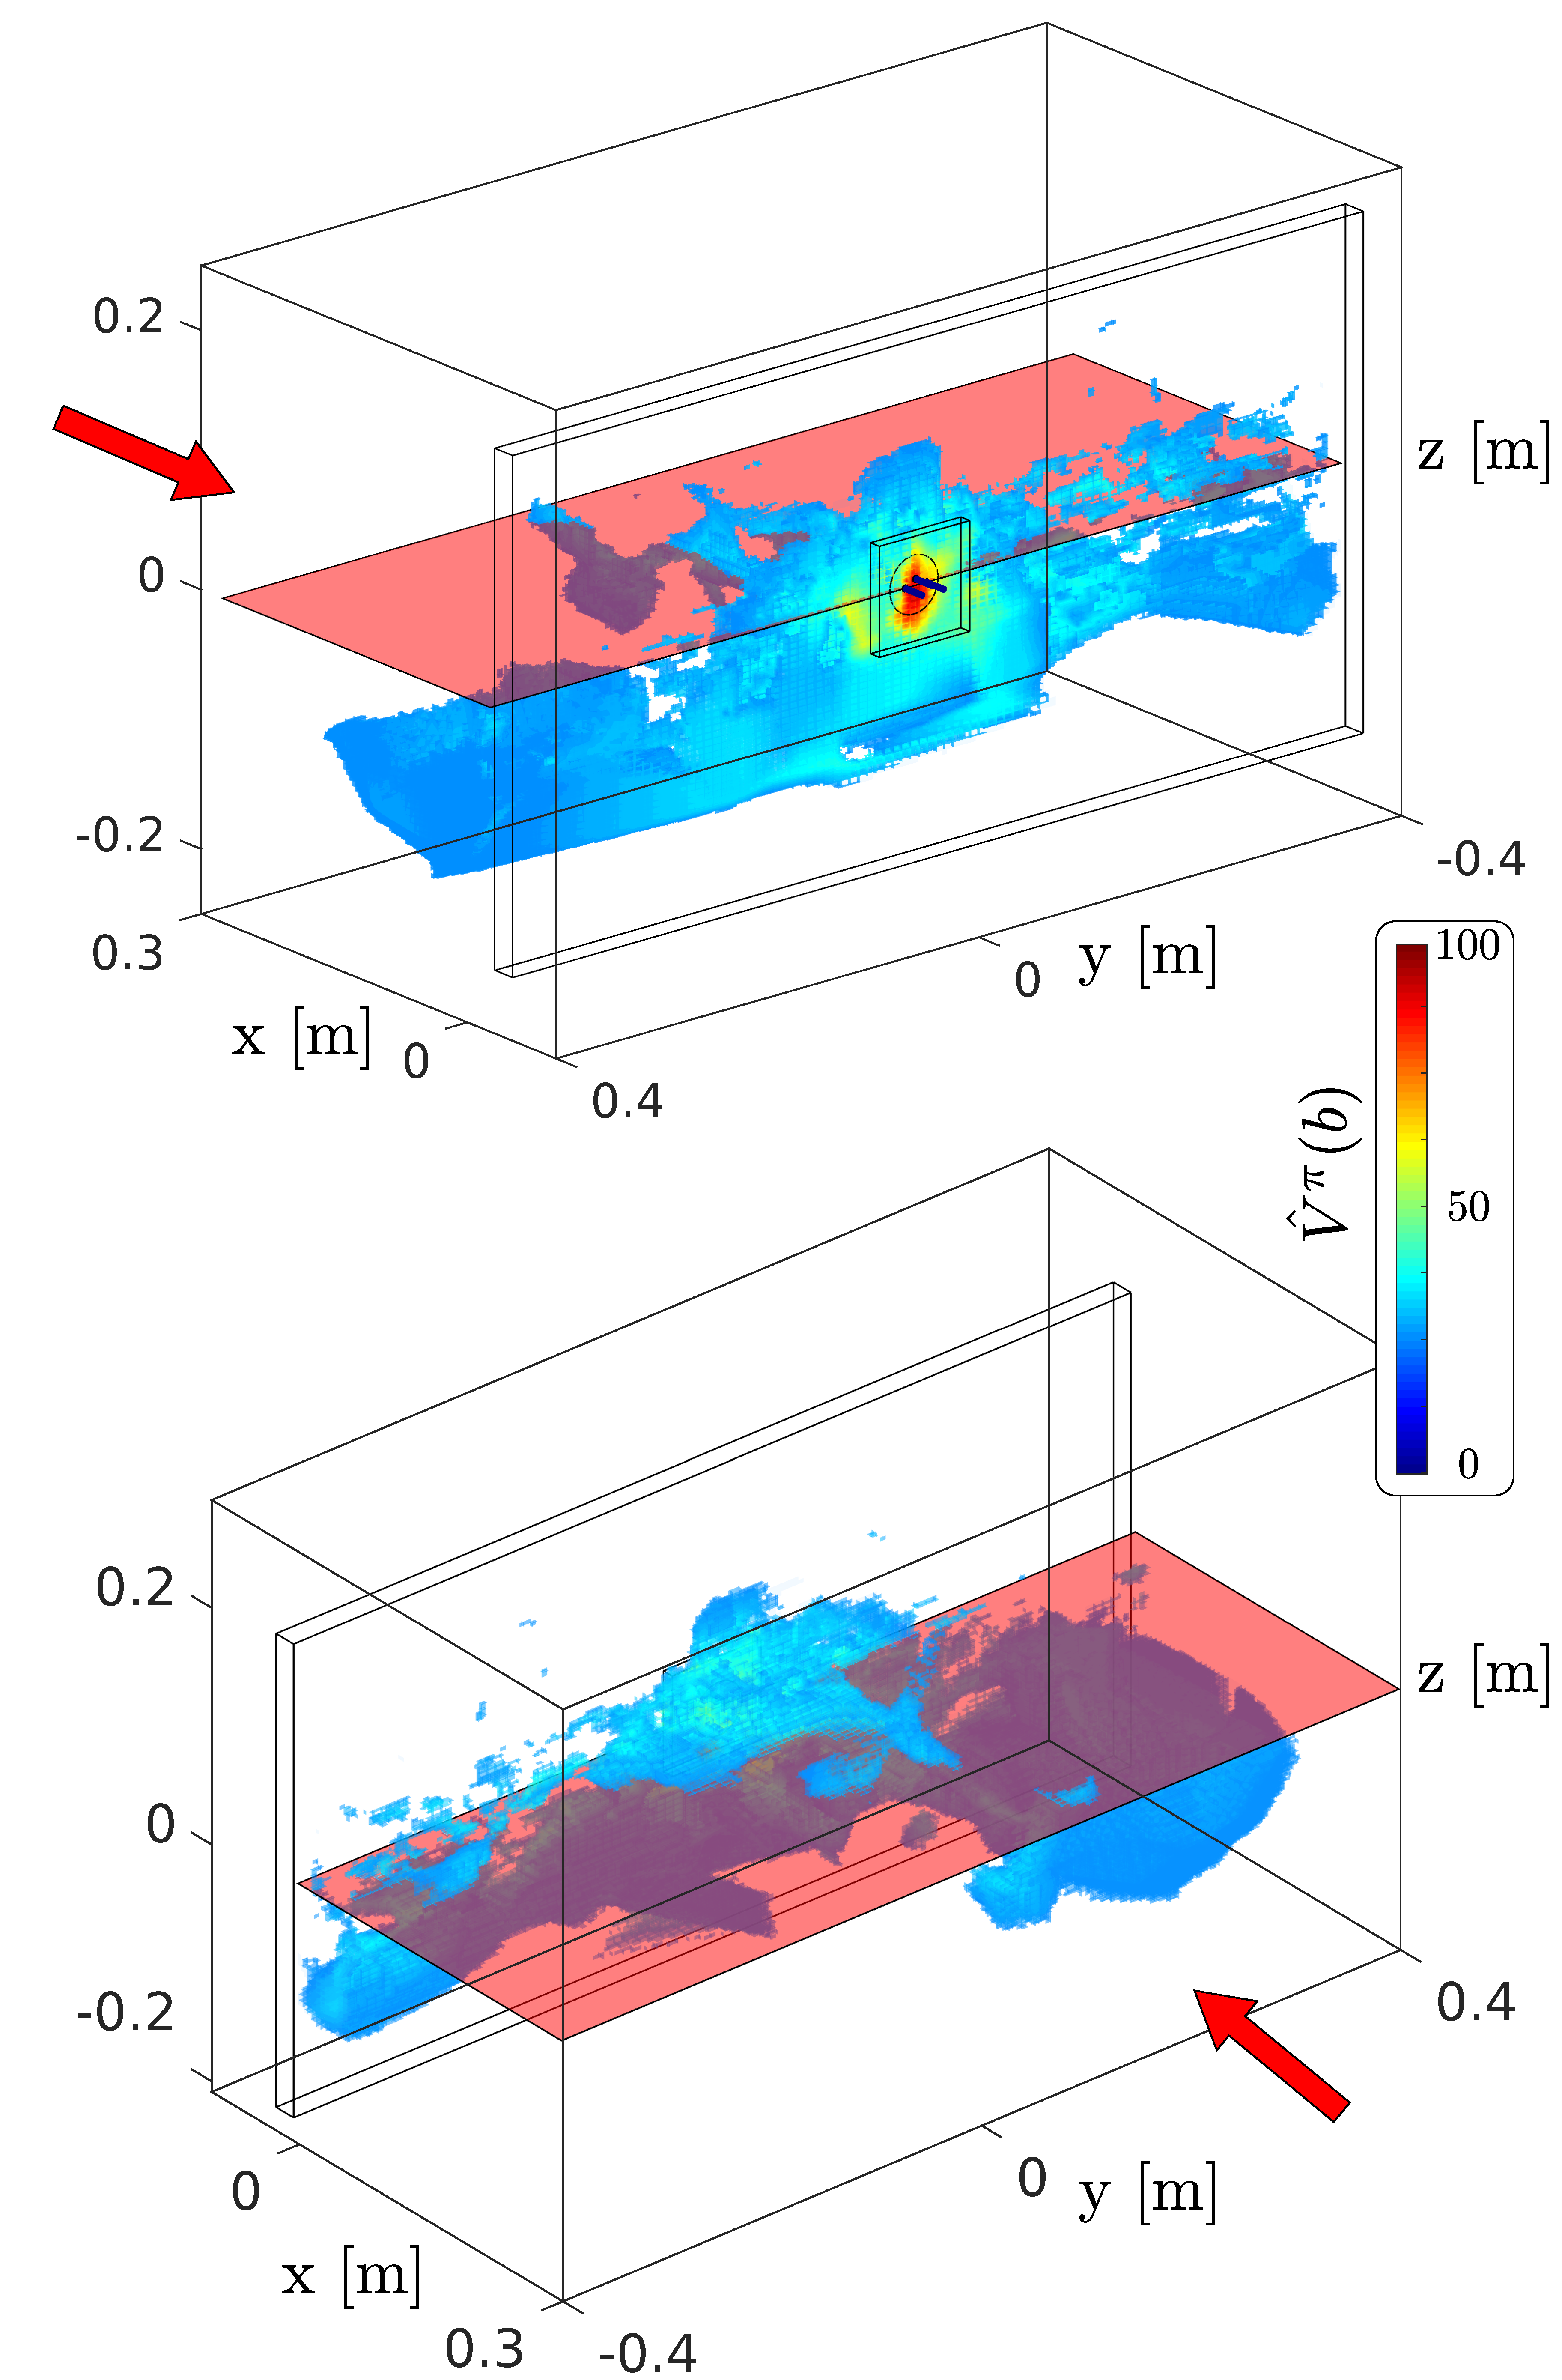
\includegraphics[width=\textwidth]{./ch4-PiH/Figures/ValueFunction/value_func_final_v2.pdf}
 \caption{LWR value function approximate $\hat{V}^{\pi}(\hat{x})$ for the most likely state $\hat{x}$. 
 The red plane is to help visualise where the value function is above and below the axis $z=0$. Only states with values above
 $0.25$ are plotted.  The red arrow indicates the heading of the human teacher when performing the search task. The discount 
 factor was $\gamma=0.99$ and the variance of the kernel variance of 1 [cm], which was set experimentally.
}
 \label{fig:ch4:Figure1}
\end{figure}

In Figure \ref{fig:best_worst_traj} we illustrate the best and worst trajectories in terms of the accumulated value function.
We can see that the five best trajectories (red) tend to be aligned with the socket (star position in front of socket), 
whilst the worst trajectories are towards the edges of the wall and tend to follow spiralling movements. 

\begin{figure}
 \centering
 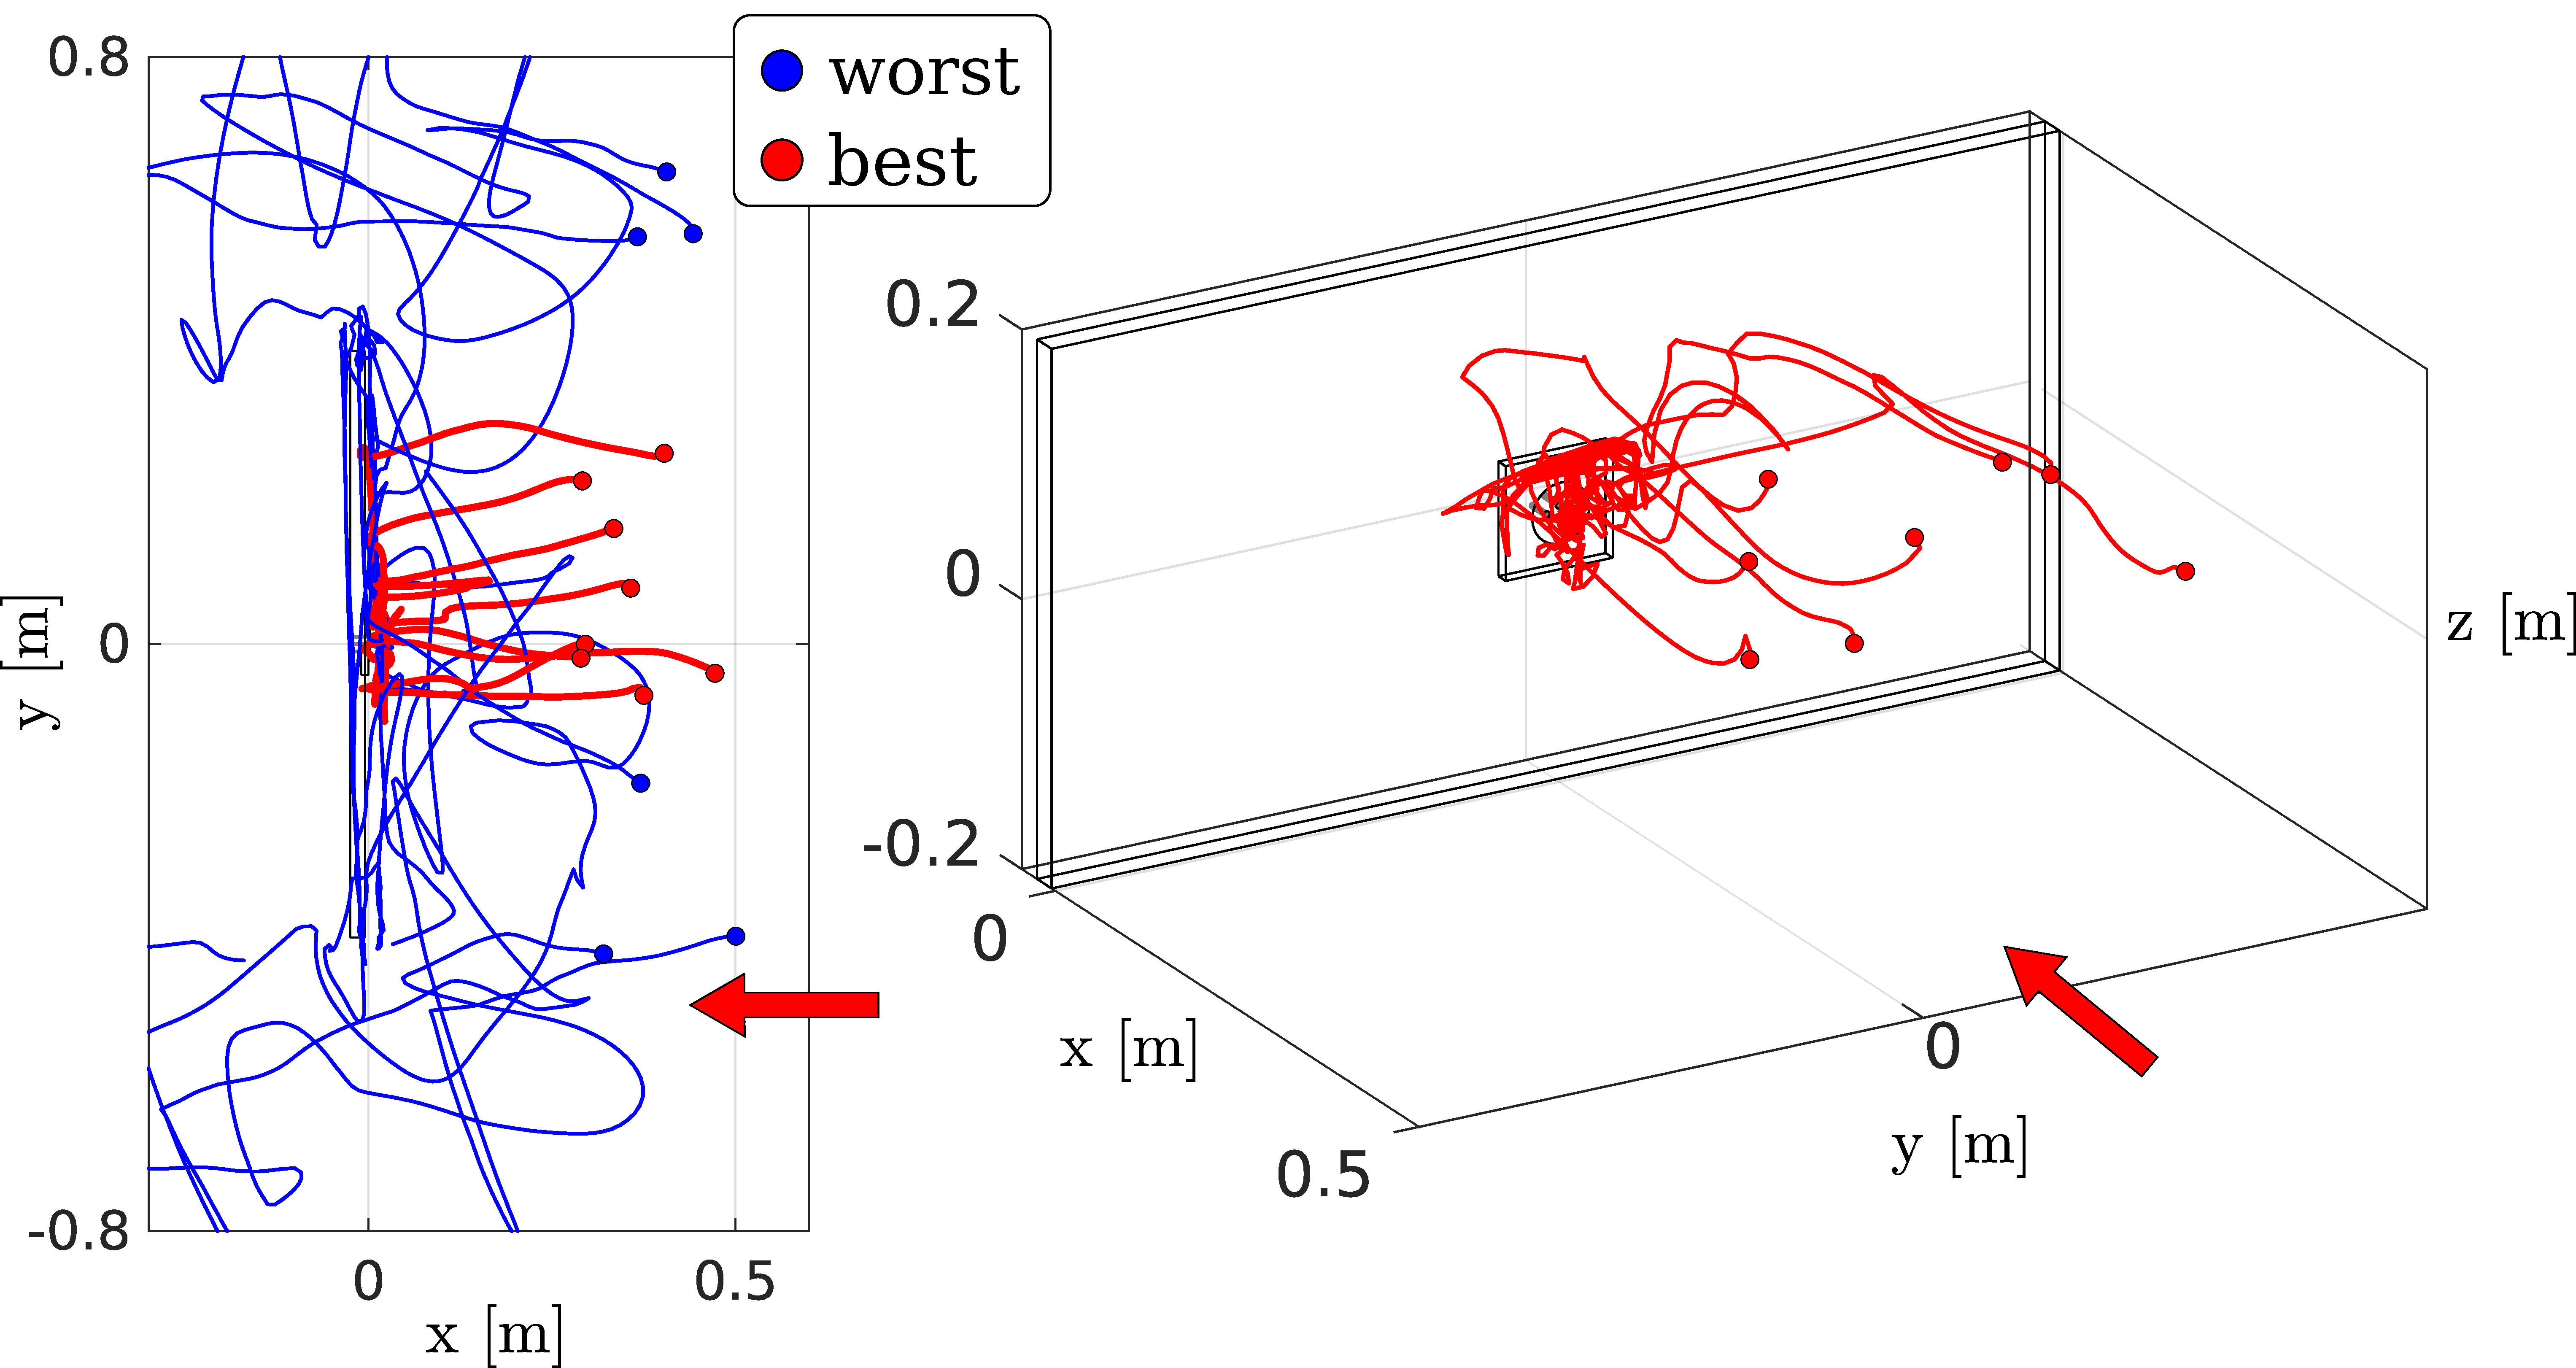
\includegraphics[width=\textwidth]{./ch4-PiH/Figures/ValueFunction/value_func_final_v3.pdf}
 \caption{Best and worst trajectories. The red demonstrated trajectories are the best in terms of the amount of value function 
 gain whilst the blue are the worst. The red arrow indicates the teacher's heading. The blue trajectories tend 
 towards the sides of the wall as the initial starting position is on the boarders of the wall. The red trajectories are centred along the y-axis of socket and tend to move in a straight line towards 
 the wall whilst aligning themselves with the axis $z=0$.} 
 \label{fig:best_worst_traj}
\end{figure}


We learned two policies, one solely from the original human demonstrations which we call GMM and the second which 
is the result of one iteration of fitted policy evaluation and improvement which we call Q-EM. In the section \ref{ch4:results}
we compare the GMM and Q-EM policies with the improvements which can be achieved within the RL-PbD-POMDP framework.

\section{Control architecture}\label{ch4:control_architecture}

As detailed in section \ref{sec:fpe}, a Gaussian Mixture Model was learned for both linear and angular velocity,
although only the linear control policy is active until the plug is within 
the socket's hole, as the orientation is constant.
The direction to search is given by the conditional, Equation \ref{eq:gmm_conditional},

\begin{equation}\label{eq:gmm_conditional}
 \pi_{\Param}(\dot{x}|b) = \sum_{k=1}^{K} w^{[k]}_{\xb} \; g(\dot{x};\MuK_{\xb},\SigK_{\xb}) 
 \end{equation}

which is a distribution over the possible normalised velocities. The function $g(\cdot)$ is a multivariate
Gaussian function parameterised by mean $\MuK_{\xb} \in \mathbb{R}^{(3\times1)}$ and Covariance $\SigK_{\xb} \in \mathbb{R}^{(3\times3)}$. The subscript $\xb$ indicates that the parameters 
are the result of the conditional. The reader is referred to \cite{gesture_calinon_2010}, \cite{gmr_2004} for 
a detailed derivation of the conditional of a GMM. The learned model 
is multi-modal, as different search velocities are possible 
in the same belief state. Figure \ref{fig:policy_vf} illustrates the multi-modal 
vector fields of the conditional, Equation \ref{eq:gmm_conditional}.
In autonomous dynamical systems control, the velocity is obtained from 
the expectation of the conditional, Equation \ref{eq:gmm_conditional}. However, the expectation which is a weighted 
linear combination of the modes, could result in unobserved behaviour or no movement if the velocities cancel out. 
As a result we use a modified version of the expectation operator which favours the current
direction, Equation \ref{eq:alpha_eq} - \ref{eq:alpha_expectation}.

\begin{align}
 \alpha(\dot{x}) &= w^{[k]}_{\xb} \cdot \exp(-\cos^{-1}(<\dot{x},\MuK_{\xb}>)) \label{eq:alpha_eq}\\
 \dot{x} &= \mathbb{E}_{\alpha}\{\pi_{\Param}(\dot{x}|b)\} = \sum_{k=1}^K \alpha_k(\dot{x}) \cdot \MuK_{\xb} \label{eq:alpha_expectation}
\end{align}

When the applied velocity mode is no longer present another direction is sampled. For example, when the robot enters in contact 
with a feature, greatly reducing the uncertainty, the current mode changes and a new search direction is computed. 
Figure \ref{fig:policy_vf} illustrates the policy vector field for GMM and Q-EM, both learned from teachers demonstrations.

\begin{figure}
   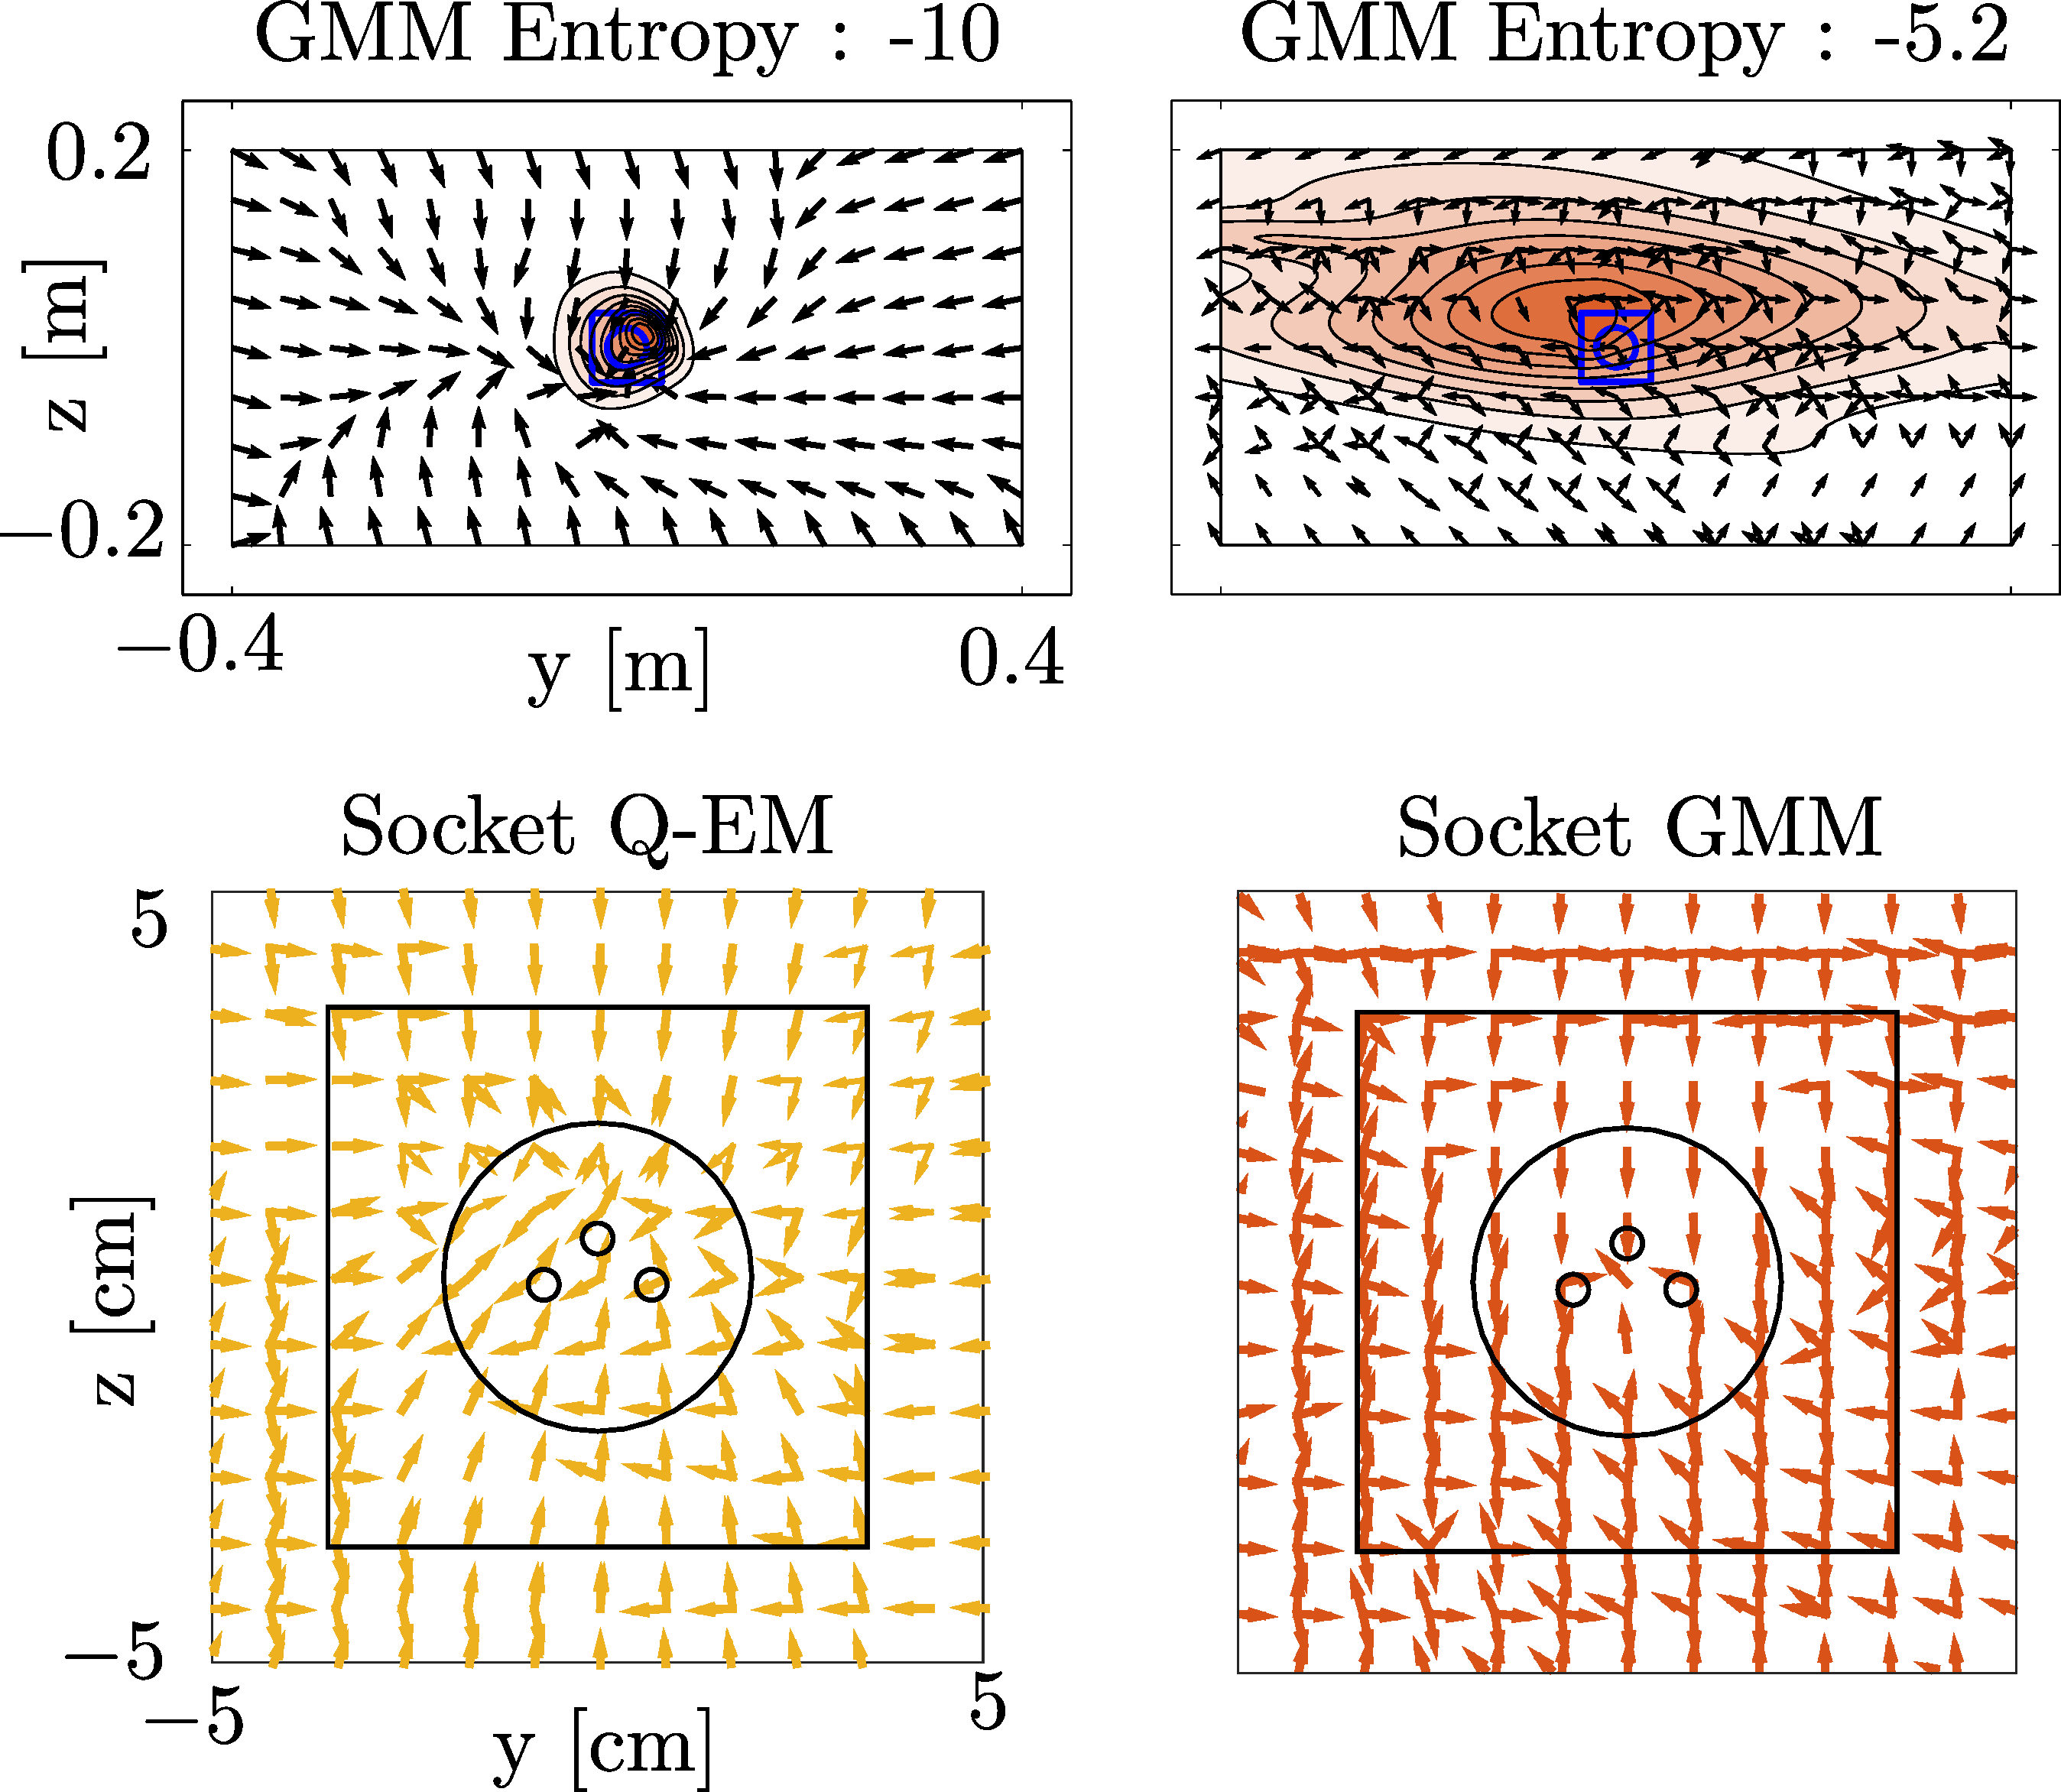
\includegraphics[width=\textwidth]{./ch4-PiH/Figures/Fig/policy_vf.pdf}
  \caption{Q-EM and GMM policy vector fields. \textit{Top}: The GMM policy is conditioned on an entropy of $-10$ and $-5.2$. For the lowest entropy level,
  most of the probability mass is close to the socket area since this level corresponds to very little uncertainty; we are already localised. We can see 
  that the policy converges to the socket area regardless of the location of the believed state. For an entropy of $-5.2$ we can see that 
  the likelihood of the policy is present across wall. The vector field directs the end-effector to go towards the left or right edge of the wall. 
  \textit{Bottom}: The entropy is marginalised out, the yellow vector field is of the Q-EM and orange of the GMM. The Q-EM vector field tends 
  to be closer to a sink and there is less variation.}
  \label{fig:policy_vf}
\end{figure}


\subsection{Robot Implementation}

The GMM policy $\dot{\underbar{x}} = \mathbb{E}_{\alpha}\{\pi_{\Param}(\dot{x}|b)\}$ outputs a linear velocity which is normalised, $\dot{\underbar{x}} \in \mathbb{R}^{(3 \times 1)}$. 
The amplitude of the velocity is computed separately and modulated according to sensed forces on the end-effector.
This search task is haptic and the end-effector of the robot is always in contact with the environment. To make the robot
compliant with the environment we use an impedance controller in combination with a hybrid position-force controller. A hybrid controller
targets a sensed force $F_x$, in the $x$-axis, of 3N. The $y$ and $z$ velocity components of the direction vector are given by 
Equation \ref{eq:alpha_expectation}. This is insufficient for the robot to reliably surmount the edges of the socket,
hence the vector field of the GMM is modulated in $y$ and $z$-axis, Equation \ref{eq:modulation}.

\begin{equation}
  \dot{\underbar{x}} = R_y(c(F_z) \cdot \pi/2) \cdot R_z(c(F_y) \cdot \pi/2) \cdot \dot{\underbar{x}} \label{eq:modulation}
\end{equation}

where $R_y$ and $R_z$ are $(3 \times 3)$ rotation matrices around the $y$ and $z$-axis, and $c(F) \in [-1,1]$ is a truncated scaling function of the sensed 
force.  When a force $F_z$ of 5N is sensed, a rotation of $R_y(\pi/2)$ is applied to the original direction resulting in the robot
getting over the edge. The direction velocity is always normalised up to this point. The amplitude of the velocity is a proportional
controller based on the believed distance to the goal,
\begin{align}
  \nu     &= \max(\min(\beta_1,K_p (x_g - \hat{x}),\beta_2)\label{eq:prop_speed}\\ \nonumber
  \dot{x} &= \nu \dot{\underbar{x}}
\end{align}
where the lower and upper amplitude limits are given by $\beta_1$ and $\beta_2$, $x_g$ is the position of the
goal, and $K_p$ the proportional gain which was tuned through trials. 

% $\omega_t = \mathrm{angleaxis}(\mathbf{R}^{\mathrm{T}} \mathbf{R}^r)$  $\mathbf{R}^r = I$

The above procedure can control the general behaviour of the search but is insufficient for a successful implementation on a robotic system 
such as the 7 Degree of Freedom $q\in\mathbb{R}^7$ KUKA LWR, which we illustrate in Figure \ref{fig:kuka}. 
The GMM policy $\dot{x} = \mathbb{E}_{\alpha}\{\pi_{\Param_1}(\dot{x}|b)\}$ outputs a linear velocity and the 
angular velocity is computed from a reference orientation which is constant. When the plug is to be connected to the socket, 
the angular velocity is the output of samples drawn from the conditional $\omega \sim \pi_{\Param_2}(\omega|\phi)$.
From both linear and angular velocities a reference position $x^r \in \mathbb{R}^{(3 \times 1)}$ and orientation $R^r \in \mathbb{R}^{(3 \times 3)}$ are computed and used to 
define a linear and angular error $x_e = x^r - x$, $\psi_e = \mathrm{angleaxis}(R^{\mathrm{T}}R^r)$ by using the  
the current position $x$ and orientation $R$.
Given the kinematic chain of the robot, the inverse of the Jacobian $J(q) \in \mathbb{R}^{6\times 7}$ is used in an impedance control to transform the 
Cartesian error $c_e = [x_e,\psi_e]^{\mathrm{T}} \in \mathbb{R}^{6 \times 1}$ to torque commands $\tau_t \in \mathbb{R}^7$, Equation \ref{eq:torque_control},

\begin{equation}\label{eq:torque_control}
 \tau_t = J^{\mathrm{T}}(q_t)\left(-K c_e - D \dot{c}_e \right) + g(q_t)
\end{equation}

where $K,D \in \mathbb{R}^{6\times6}$ are diagonal stiffness and damping matrices whose values were set experimentally 
and $g(q_t)$ compensates for gravity. Given an applied torque there is a resulting joint velocity $\dot{q}_t$ from which we can compute the measured Cartesian end-effector velocity used in the motion model of the PMF.
Figure \ref{fig:control_flow} illustrates the complete control flow.

\begin{figure}
 \centering
 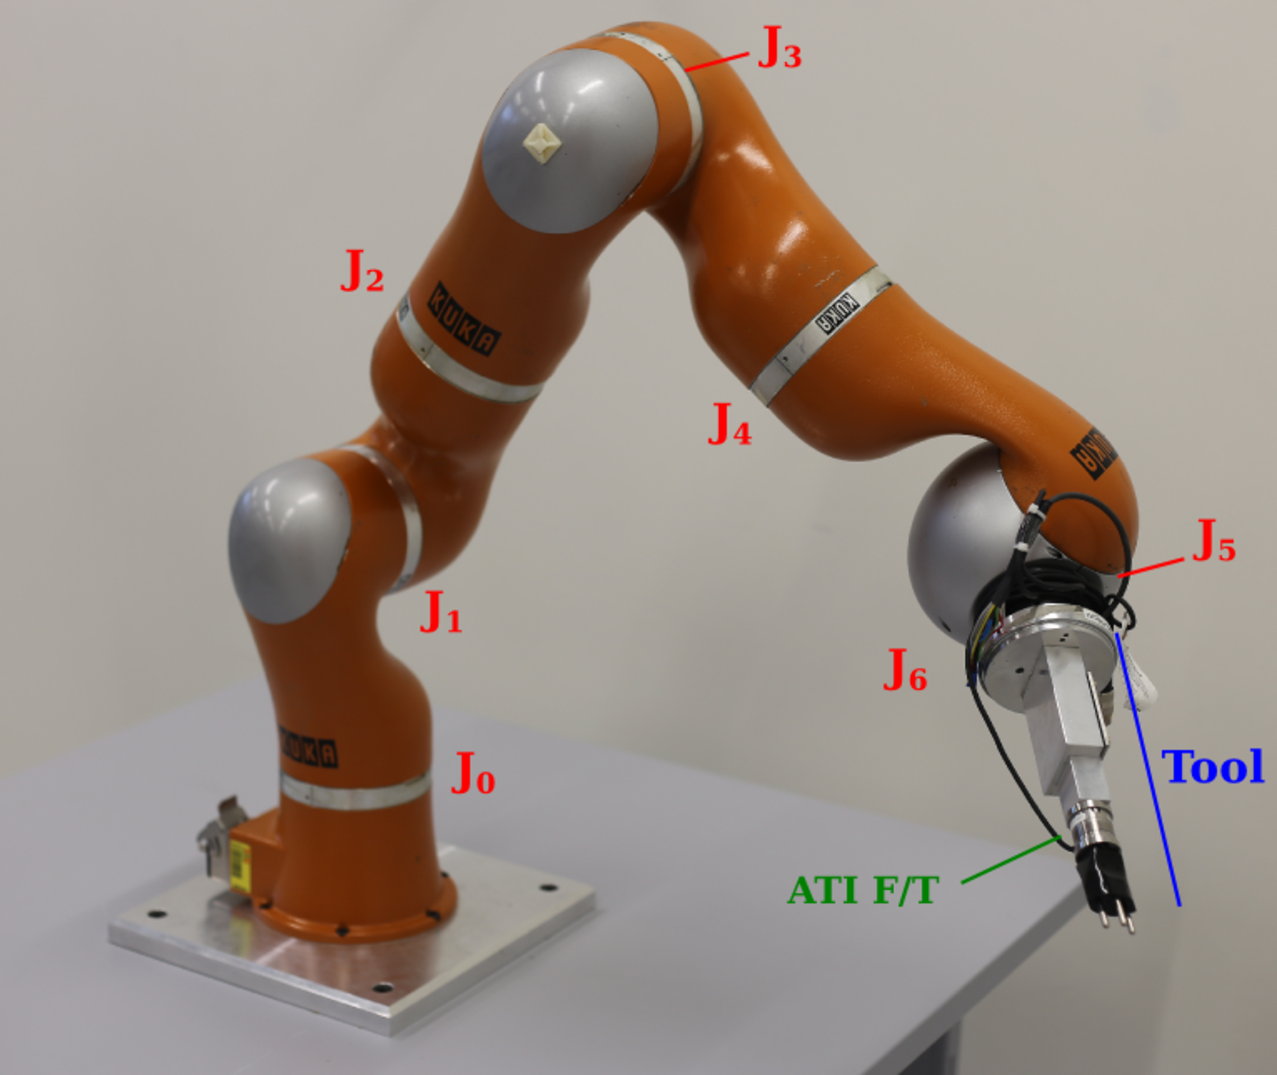
\includegraphics[width=0.8\textwidth]{./ch4-PiH/Figures/kuka.pdf}
 \caption{The KUKA LWR is a 7 Degree Of Freedom (DoF) robot, we illustrate in red each joint, which is controlled at a rate of 1kHz via an ethernet cable. The KUKA API provides a command interface to the 
 stiffness, damping, position and torque variables of each joint.}
 \label{fig:kuka}
\end{figure}

\begin{figure}
  \centering
  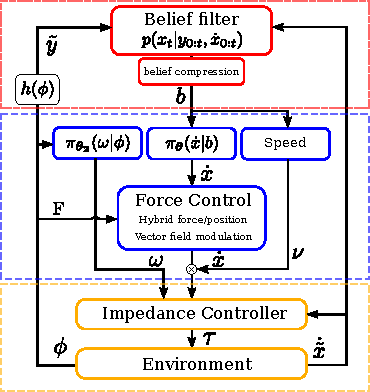
\includegraphics[width=0.8\textwidth]{./ch4-PiH/Figures/control_flow_final.pdf}
  \caption{Control architecture. The PMF (belief) receives a measured velocity, $\dot{\tilde{x}}$, and 
  a sensor measurement $\tilde{y}$ and is updated via Bayes rule. The belief is compressed and used by both the GMM policy and the proportional speed controller, Equation \ref{eq:prop_speed}.}
  \label{fig:control_flow}
\end{figure}


\FloatBarrier
\section{Results}\label{ch4:results}

We evaluate the following three aspects of the policy learned in our Actor-Critic framework:
\begin{enumerate}
 \item \textbf{Distance taken to accomplish the goal} (connect plug to socket). We compare the Q-EM policy with 
 a GMM policy learned through standard EM and a myopic Greedy policy. This highlights the difference between complicated and simplistic  
  search algorithms and gives an appreciation of the problem's difficulty.
 \item \textbf{Importance of data} provided by human teachers. We evaluate whether it is possible to learn 
 an improved GMM policy from Greedy demonstrations. This policy which we call Q-Greedy is used to test whether 
 indeed human demonstrations are necessary.
 We evaluate whether it is possible to obtain a good policy from the two worst teachers' demonstrations as not all teachers 
 are necessarily proficient at the task in question and we want to test whether our methodology can be applied in these
 cases. We evaluate if we  are able to obtain an improved policy from the worst two teachers.
 \item \textbf{Generalisation}. We learn a policy to insert a plug into socket A which is located at the center of a wooden 
 wall. We test the generalisation of the policy in finding a new socket location and whether the policy can generalise to sockets 
 B and C, which were not used during the training phase.
\end{enumerate}

We evaluate aspects 1) and 2) purely in simulation as finding the socket requires much less precision than establishing a 
connection and the physics of the interaction is simple. Aspect 3), the generalisation, is evaluated both in simulation,
up to the point of localising the socket's edge, and on the KUKA LWR robotic platform
for the connection phase of the task. The main reason for employing the robot is that the connection phase dynamics is 
complex and a simulation would be unrealistic. For the robot evaluation we consider 
the search starting already within the vicinity of the socket.


%We evaluate the above properties under two separate conditions. In the \textbf{first condition} we consider the period between the start 
%of the search until the socket is localised. In the \textbf{second condition} we consider the period from the point the socket is found until
%a connection has been established. In the first condition the evaluation is done in simulation whilst 
%in the second condition, when the socket is found, we perform the evaluation with a physical robot, the KUKA LWR4.

%This choice is motivated by the fact that the two parts of the task require different levels of precision.
%Finding the socket requires much less precision than establishing a connection. It is more informative to consider the performance of these two parts separately.
%Another aspect is that the search for the socket can be reliably evaluated in simulation since the physics of the interaction
%is simple. The connection phase is more complicated and a simulation would be unrealistic.

\subsection{Distance taken to reach the socket's edge (Qualitative)}

We consider three search experiments which we refer to as \textbf{Experiment 1, 2} and \textbf{3},
in order to evaluate the performance in terms of the distance travelled to reach the socket for the three search policies: GMM, Q-EM and Greedy.
In these three experiments the task is considered accomplished when a search policy finds the socket's edge. 

In \textbf{Experiment 1}, three starting locations are chosen: \textit{Center}, \textit{Left} and \textit{Right}. 
See Figure \ref{fig:box_exp_sim}, \textit{Experiment 1}, for an illustration of the initial condition. 
This setup tests the effect of the starting positions. A total of 25 searches are carried out for each of the search policies.

In \textbf{Experiment 2}, two \textit{Cases} are chosen in which the believed state (most likely state of the PMF) and the true position
of the end-effector are relatively far apart. The location of the beliefs are chosen to be symmetric, see the Figure \ref{fig:box_exp_sim}, 
\textit{Experiment 2}. A total of 25 searches are carried for each of the two cases.

In \textbf{Experiment 3}, Figure \ref{fig:box_exp_sim}, \textit{Experiment 3}, the initial true starting positions 
of the end-effector are taken from a regular grid covering the whole start region, also used as the initial distribution for 
the human demonstrations. A total of a 150 searches are carried out for each of the three policies. 
This experiment compares the search policies with the human teachers' demonstrations.

\begin{figure}
    \centering
    \hspace*{-1.4cm}
    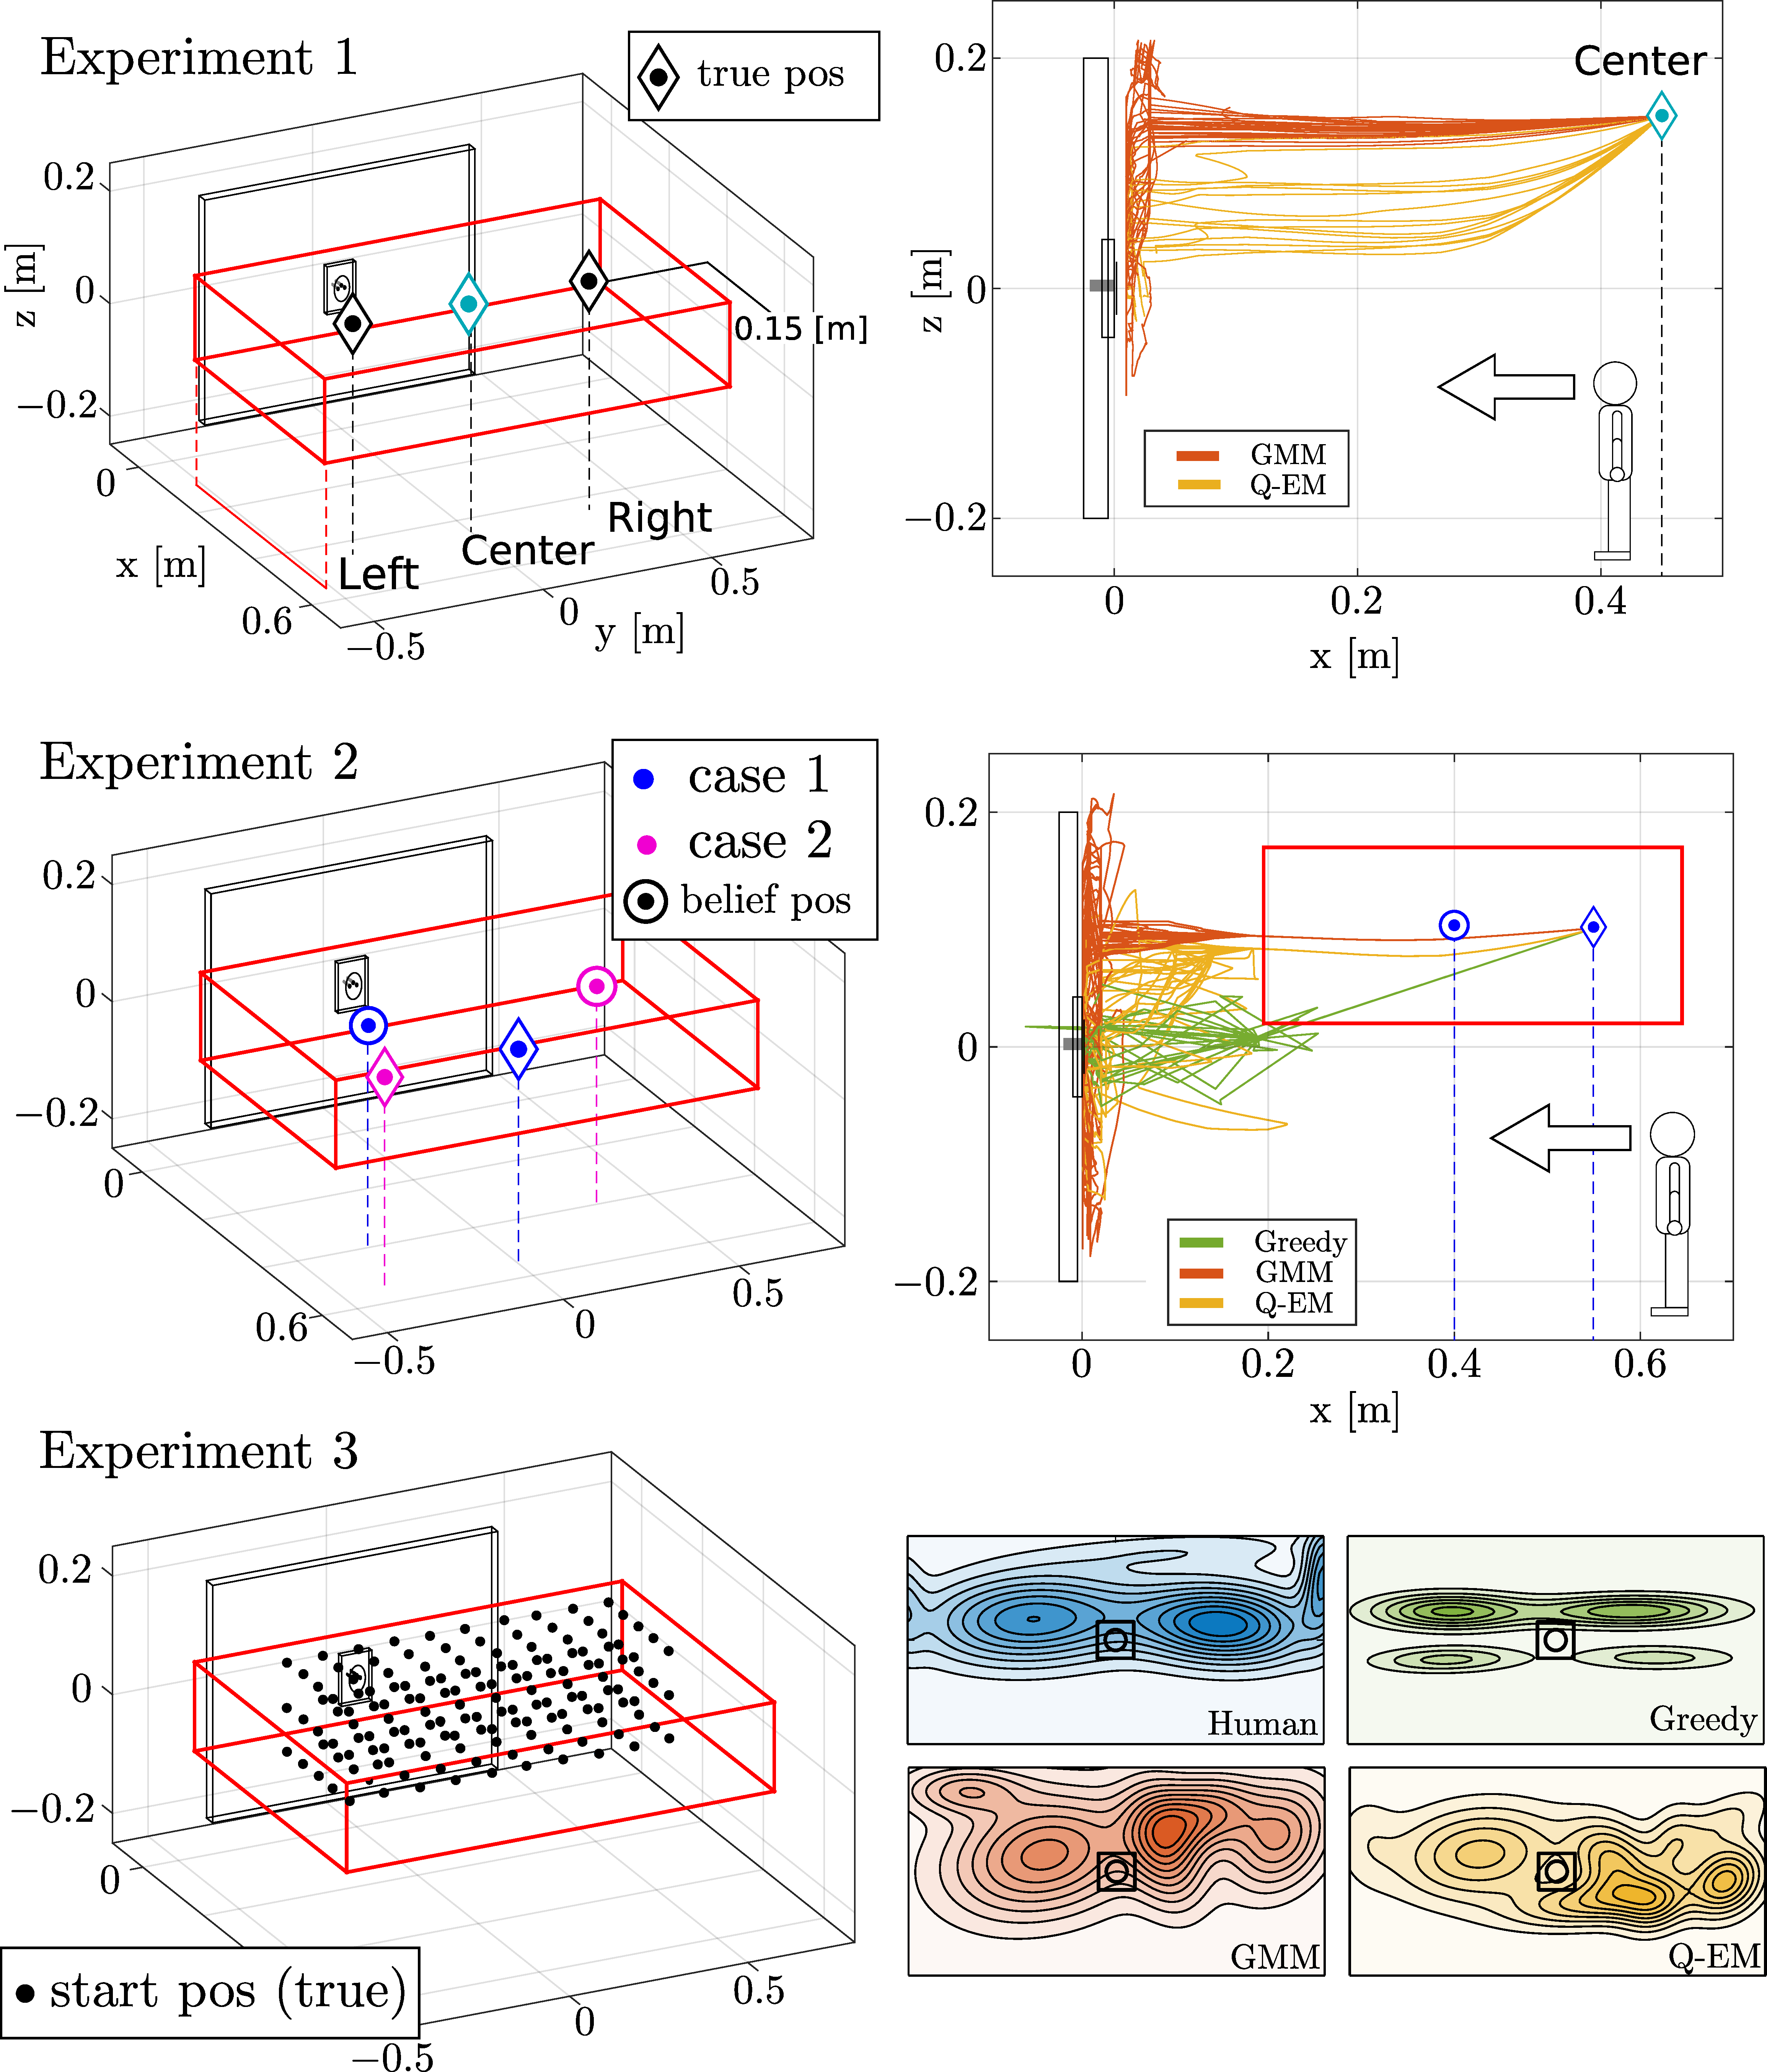
\includegraphics[width=1.2\textwidth]{./ch4-PiH/Figures/Fig/experiment_final_v3.pdf}
    \caption{Three simulated search experiments. \textbf{Experiment 1:} Three start positions are considered: \textit{Left}, \textit{Center} and
     \textit{Right} in which the triangles depict true position of the end-effector. The red cube illustrates the extent of the uncertainty. 
     In the second row of Experiment 1, we illustrate the trajectories of both the GMM (orange) and Q-EM (yellow) policies. For each start condition 
     a total of 25 searches were performed for each search policy. 
     \textbf{Experiment 2:} Two cases are considered: \textit{Case 1} blue, the initial belief state (circle) is fixed facing 
     the left edge of the wall and the true location (diamond) is facing the socket.
     \textit{Case 2} pink, the initial belief state (circle) is fixed to the right facing the edge of the wall and the 
     true location is the left edge of the wall. In the second row, the trajectories are plotted for \textit{Case 1}.
     \textbf{Experiment 3:} A 150 start locations are deterministically generated from a 
     grid in the start area. In the second row, we plot the distribution of the areas visited by the true position during the search.}
    \label{fig:box_exp_sim}
\end{figure}

We evaluate the performance of the three experiments in terms of the trajectories and their distribution in reaching 
the edge of the socket. 

In \textbf{Experiment 1}, see Figure \ref{fig:box_exp_sim} \textit{Experiment 1, second row} the results show 
a clear difference between the trajectories generated by the GMM and Q-EM policies. The orange GMM policy trajectories 
go straight towards the wall, whilst the yellow Q-EM policy trajectories drop in height making them closer 
to the socket. The same effect can be seen in Experiment 2 (\textit{second row}). The Q-EM trajectories 
follow a downward trend towards the location of the socket. The gradient is less as the initial starting condition is 
lower than in Experiment 1. 

In \textbf{Experiment 2}, see Figure \ref{fig:box_exp_sim}, \textit{Experiment 2, second row}, 
the trajectories of the Greedy policy depend on the chosen believed location (most likely state of the PMF). There 
is no variance in the Greedy's trajectories until it reaches the edge of the red square, where the branching 
occurs as the believed location is disqualified. This happens as no sensation has been registered at the point 
when the believed location reaches the wall. The true location is in fact situated further away from the wall 
than the believed location.

In \textbf{Experiment 3}, see Figure \ref{fig:box_exp_sim} \textit{Experiment 3, second row}, Human and GMM show 
similar distributions of searched locations. They cover the upper region of the wall and top corners, to 
some extent. These distributions are not identical for two reasons. The first is that the learning of the GMM is a 
local optimisation which is dependent on initialisation and number of parameters. The second reason is that 
the synthesis of trajectories from the GMM is a stochastic process. 

For the  Q-EM policy, the distribution of the searched locations is centred around the origin of the $z$-axis.
The uncertainty is predominantly located in the $x$ and $y$-axis. The Q-EM policy takes this uncertainty 
into consideration by restraining the search to the $y$-axis regardless of the starting position. The uncertainty 
is reduced when it is in the vicinity of the socket. 
The Greedy's policy search distribution is multi-modal and centred around the $z$-axis where the modes are above 
and below the socket. This shows that the Greedy policy acts according to the most likely state 
which changes from left to right of the socket, because of motion noise, resulting in left-right 
movements and little displacement. As a result the Greedy policy spends more time at these modes.

In Figure \ref{fig:first_contact} (\textit{Top-left}), we illustrate the distribution of the first contact with the wall 
during Experiment 1 for the \textit{Center} initial conditions. The distribution of the first contact of the Greedy method is uniform across 
the entire $y$-axis of the wall. 
It does not take into account the variance of the uncertainty. In contrast, the GMM policy remains centred with respect to the starting position and the Q-EM is even closer to the socket and 
there is much less variance in the location of the first contact.

\begin{figure}
  \centering
   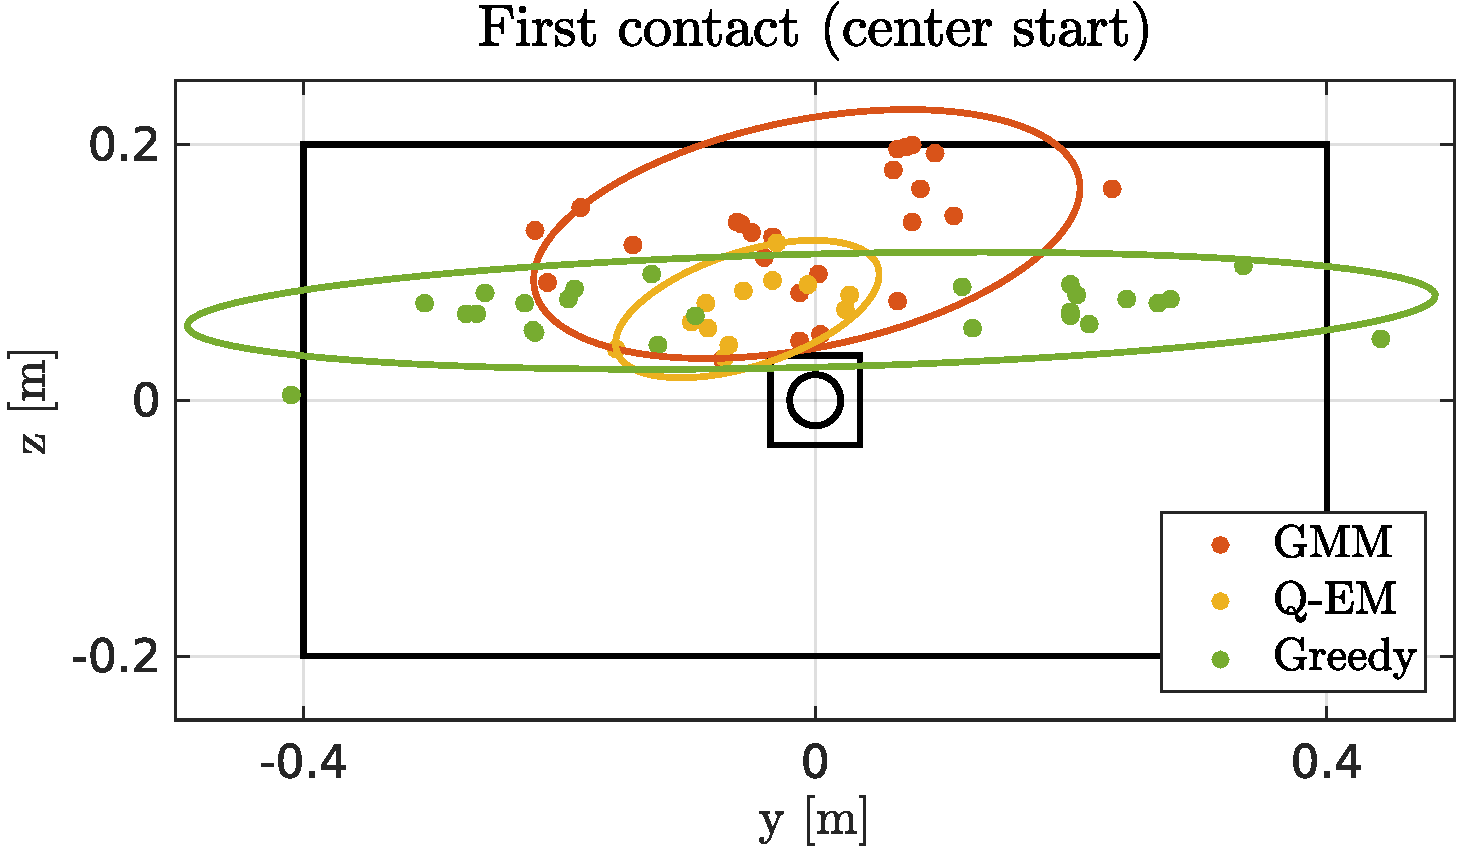
\includegraphics[width=0.45\textwidth]{./ch4-PiH/Figures/Fig/first_contact_center.pdf}
   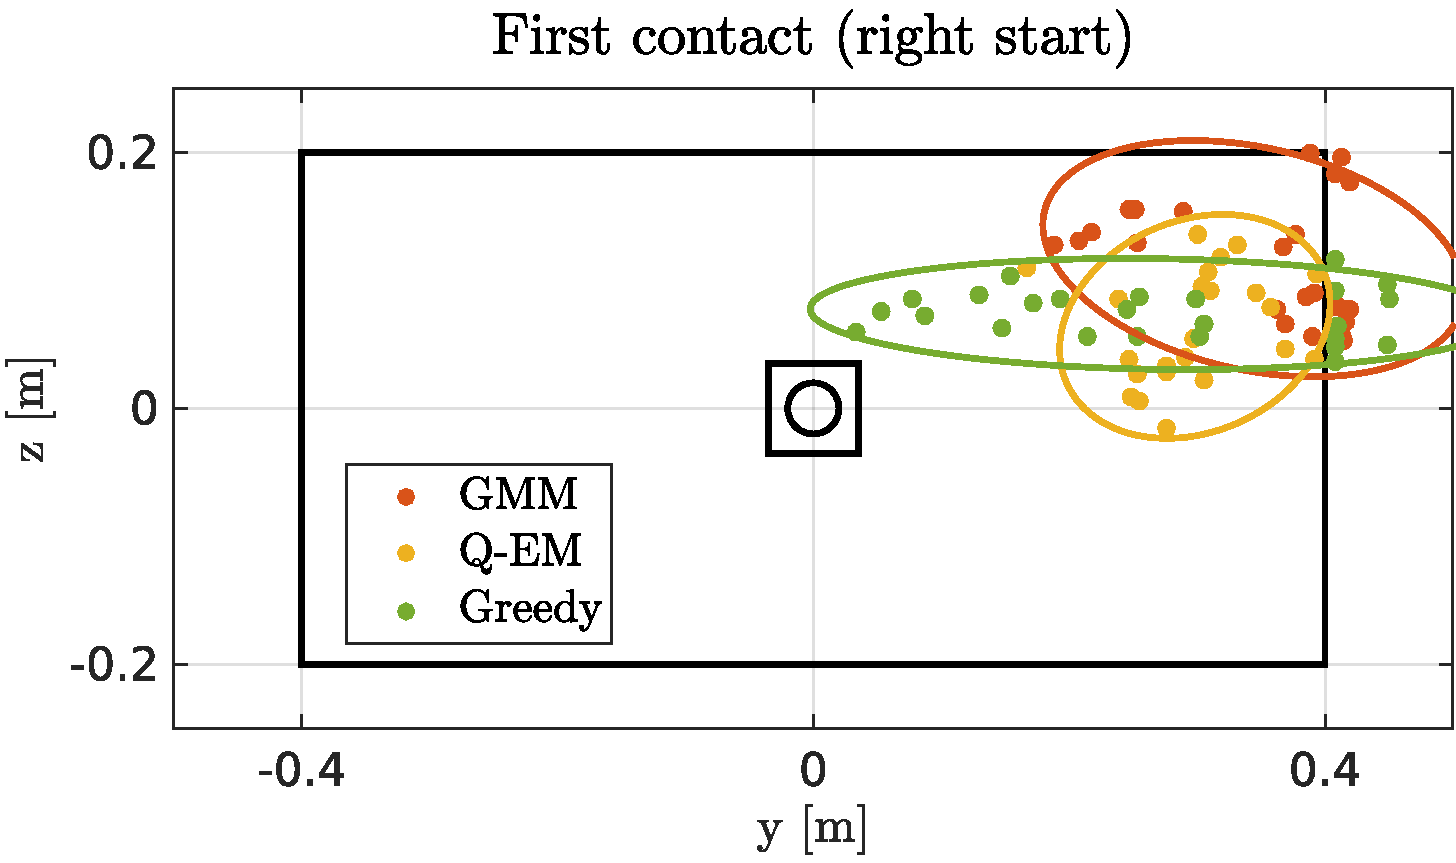
\includegraphics[width=0.45\textwidth]{./ch4-PiH/Figures/Fig/first_contact_right.pdf}
   \caption{First contact with the wall, during experiment 1. (a) Contact distribution for initial condition ``Center'' . (b) 
   Contact distribution for initial condition was ``Right''. The ellipses correspond to two standard deviations of a fitted Gaussian 
   function.}
   \label{fig:first_contact}
\end{figure}

\subsection{Distance taken to reach the socket's edge (Quantitative)}

In Figure \ref{fig:three_searches} we illustrate the quantitative results of the distance taken 
to reach the socket for all three experiments. In \textbf{Experiment 1}, for the \textit{Center} initial condition,
the Q-EM policy travels far less than the other search policies. Considering that the initial position of the search is 
0.45 [m] away from the wall, the Q-EM policy finds the socket very quickly once contact has been established with the wall. 
For the \textit{Right} and \textit{Left} starting conditions both the GMM and Q-EM policies travel less distance to reach the socket, with a 
smaller variance when compared with the Greedy search policy.

In \textbf{Experiment 2}, Figure \ref{fig:three_searches}, the Q-EM search policy is the most efficient. For \textit{Case 1} 
of Experiment 2, the initial most likely state is fixed to the left and the true position is facing the socket. 
As the belief is chosen to be to the left, upon contact with the wall the policy takes a left action since it 
is more likely to result in a localisation. 
On average this results in an exploration of the upper left area of the wall, which explains why \textit{Case 1} of Experiment 2 
performs worse than Experiment 1 for the \textit{Center} initial condition. In \textit{Case 2} however, where the 
true state is facing the left edge and the believed position is facing the right edge, less distance is taken to find the 
socket than for \textit{Case 1}, Figure \ref{fig:three_searches} (b). This improvement over \textit{Case 1} is due to the true location of 
the end-effector being closer to an informative feature and results in a much faster localisation.

From \textbf{Experiment 3}, Figure \ref{fig:three_searches_exp3}, it is clear that all three search policies travel 
less to find the socket's edge compared with the teachers' demonstrations. 
All search policies are better than the human teachers with the exception of group B\textsuperscript{*}, 
which is performing the task with socket A. The Q-EM policy remains the best. 

\begin{figure}
 \centering
  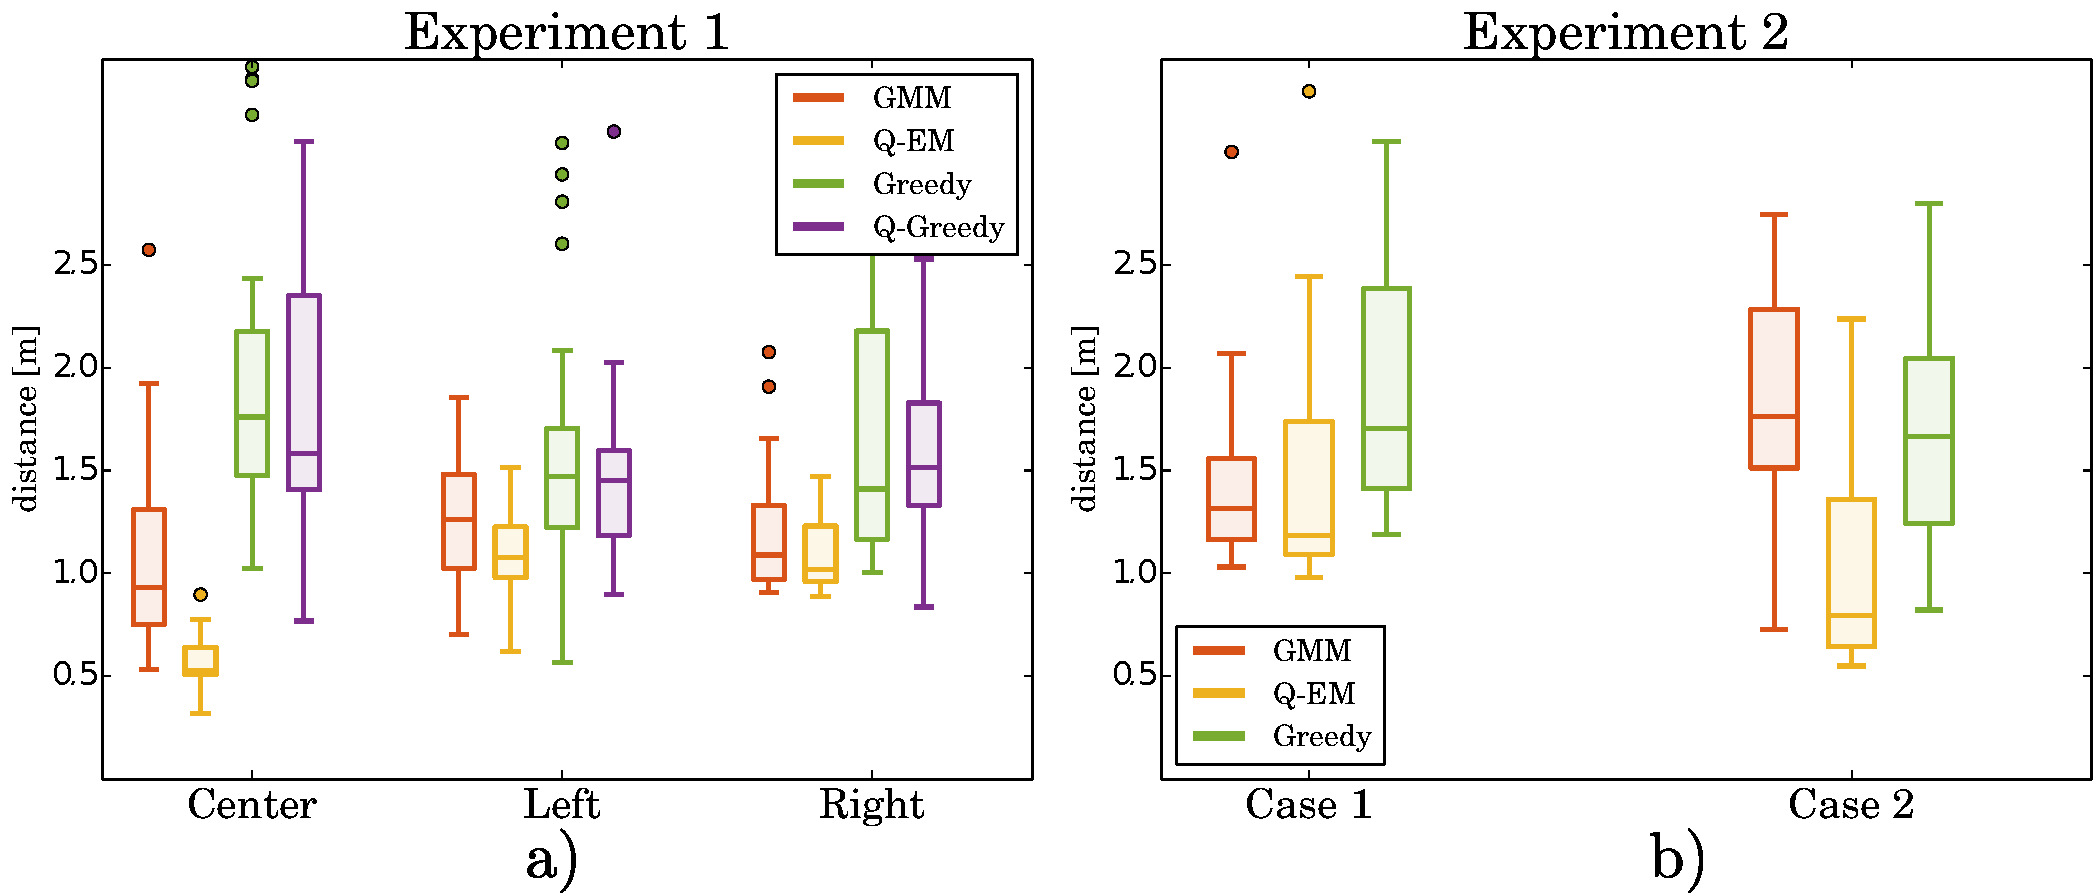
\includegraphics[width=\textwidth]{./ch4-PiH/Figures/Fig/experiment_1_2.pdf}
  \caption{Distance travelled until the socket's edge is reached. a) Three groups correspond to the initial conditions: Center, Left and Right
   depicted in Figure \ref{fig:box_exp_sim}, \textit{top left}. The Q-EM method is always better than the other methods, in terms of distance. b)
   Results of the two initial conditions depicted in Figure \ref{fig:box_exp_sim}, \textit{top middle}, both the true position and most likely state are
   fixed. The Q-EM method always improves on the GMM. }
   \label{fig:three_searches}
\end{figure}
\begin{figure}
 \centering
  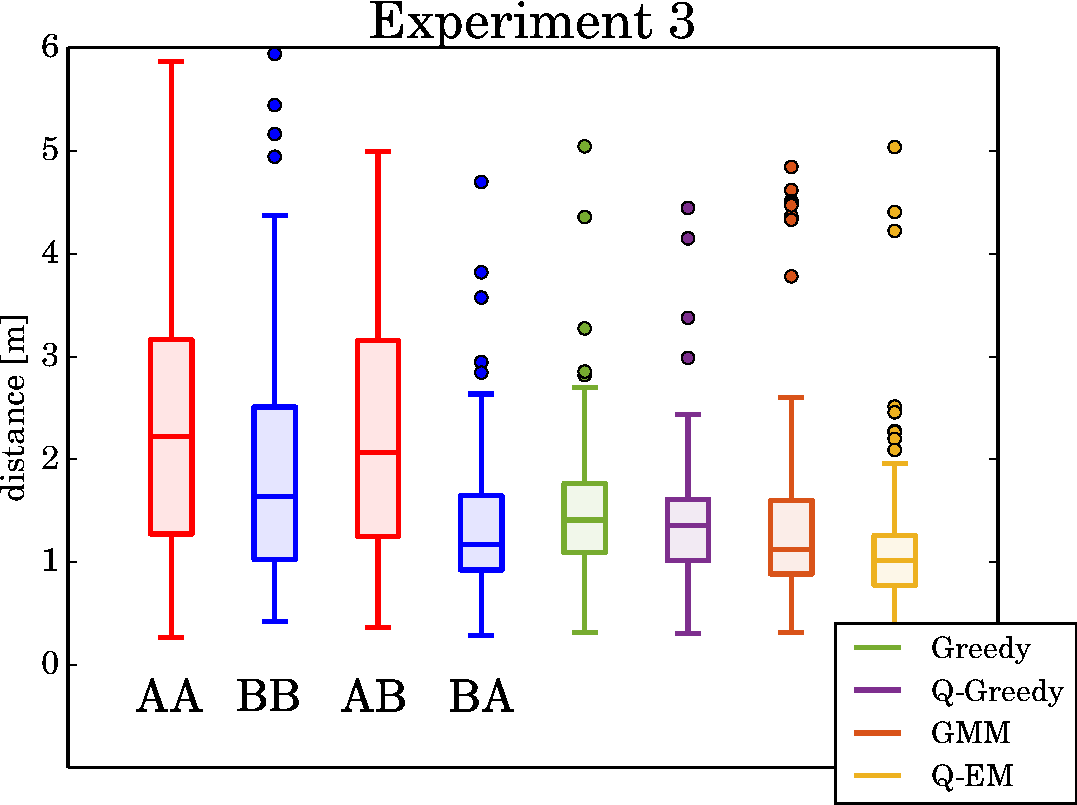
\includegraphics[width=0.6\textwidth]{./ch4-PiH/Figures/Fig/experiment3_plot2.pdf}
  \caption{Distance travelled until the socket's edge is reached. Results corresponding to Experiment 3, Figure \ref{fig:box_exp_sim}, \textit{top right}.
   Again the Q-EM method is better, but at a less significant level.}
   \label{fig:three_searches_exp3}
\end{figure}
 

We have shown that under three different experimental settings the Q-EM algorithm is predominantly the best in terms of distance taken 
to localise the socket. The GMM policy learned solely from the data provided by the human teachers also performs well in comparison to  
the human teachers and Greedy policy. We made, however a critical assumption in order to be able to use our (RL-)PbD-POMDP approach. 
This \textbf{assumption} is that a human teacher is proficient in accomplishing the task. If a teacher is not able to accomplish 
the task in a repetitive and consistent way so that a search patter can be encoded by the GMM, the learned policy will perform poorly.
Next we evaluate the validity of this assumption and the importance of the training data provided by the human teachers.
% 
\subsection{Importance of data}

We perform two tests to evaluate the importance of the teachers training data for learning a search policy. Firstly we take the 
worst two teachers in terms of distance taken to find the socket's edge and learn a GMM and Q-EM policy separately from their 
demonstrations. In this way we can evaluate whether it is possible to learn a successful policy given 
a few bad demonstrations (15 training trajectories for each policy). Our second evaluation consists of using a noisy 
explorative Greedy policy as a teacher to gather demonstrations which can then be used to learn a new policy, which we call Q-Greedy. 

Figure \ref{fig:subj_5_traj} illustrates 6 trajectories of teacher \# 5. The human teacher preferred to
localise himself at the top of the wall before either proceeding to a corner or going directly towards the socket. Once localised, the teacher 
would reposition himself in front of the socket and try to achieve an insertion. This behaviour was not expected 
since by losing contact with the wall, the human teacher no longer had sensory feedback necessary 
to maintain an accurate position estimate.

\begin{figure}
 \centering
    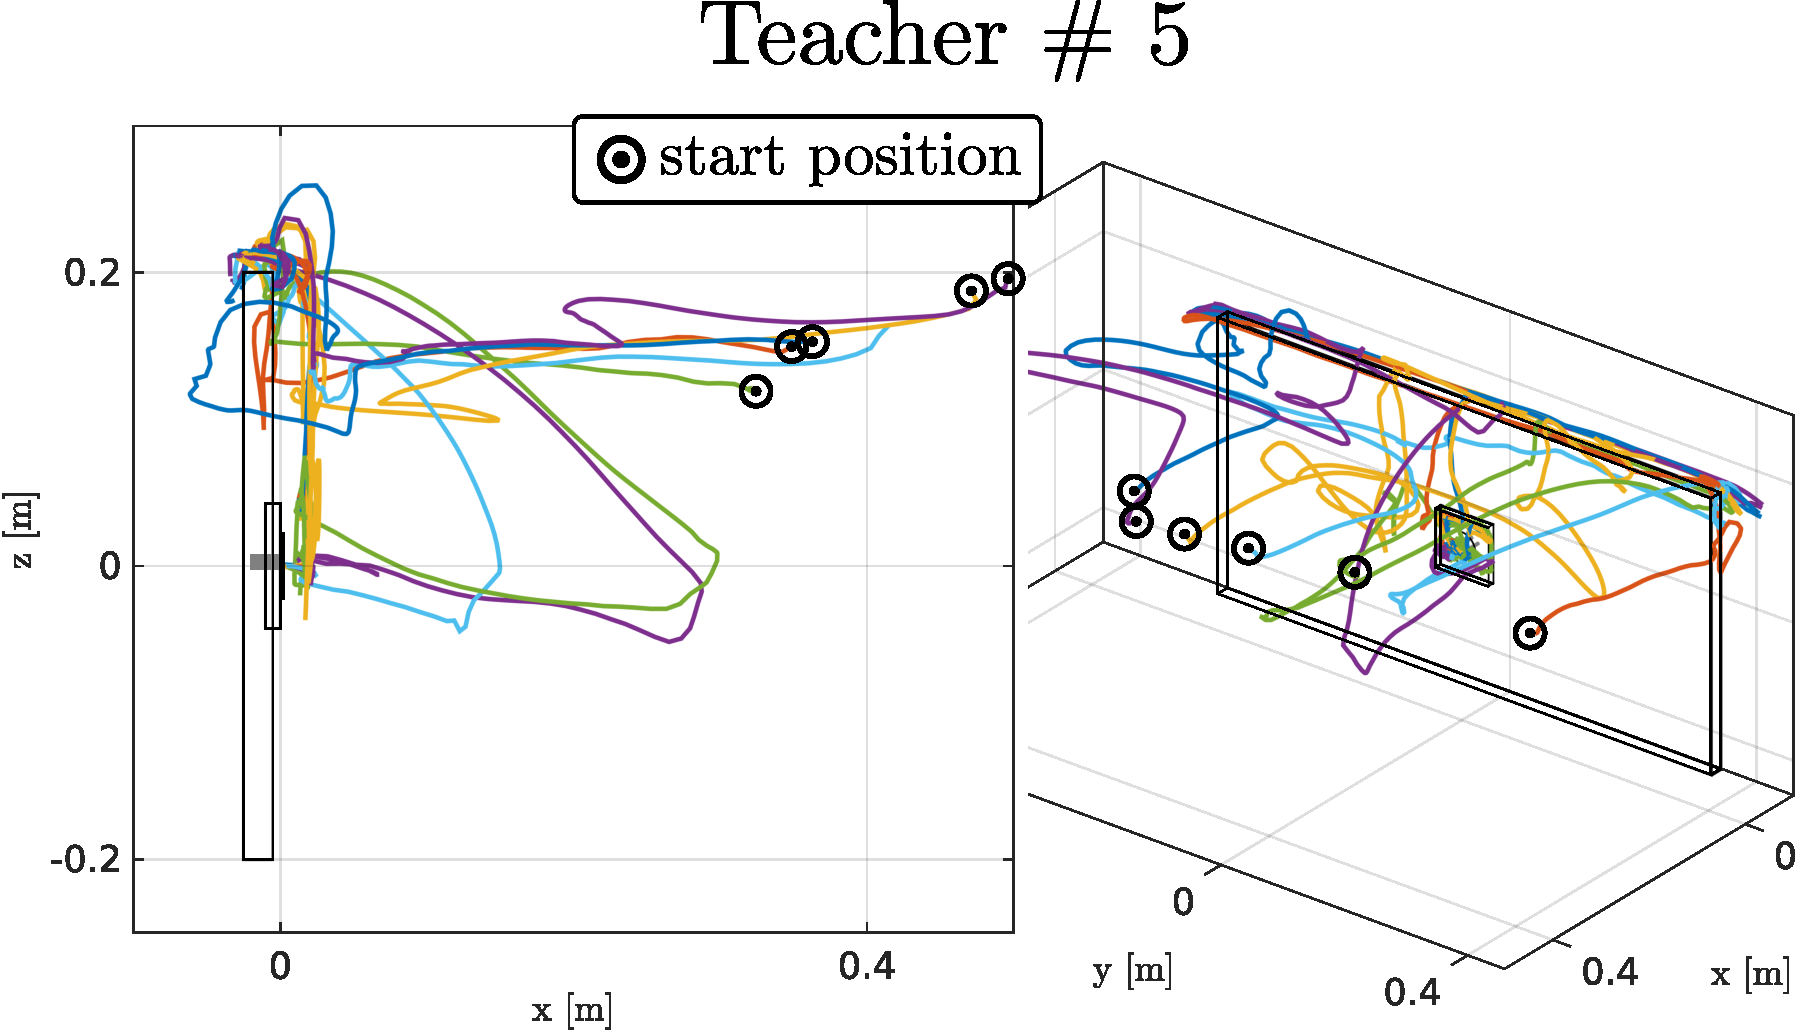
\includegraphics[width=\textwidth]{./ch4-PiH/Figures/Fig/subject5.pdf}
%    \subfigure[]{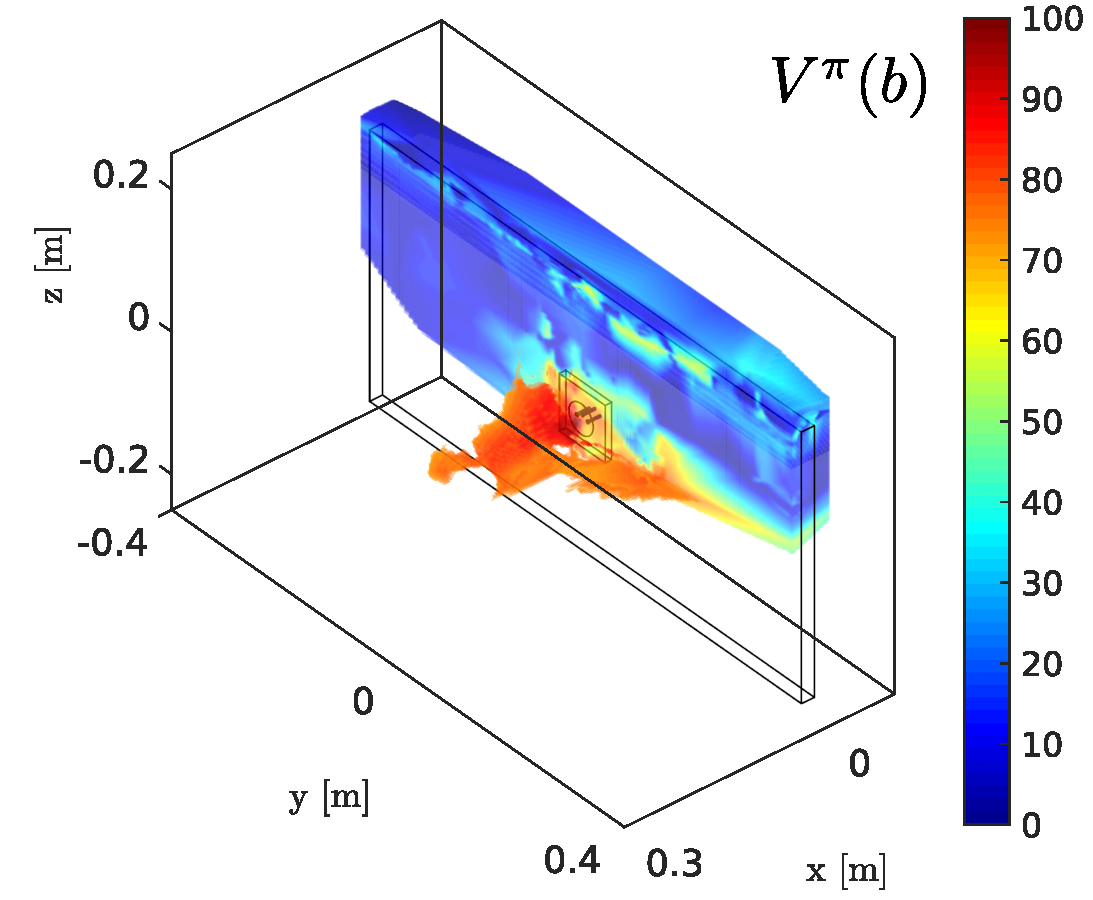
\includegraphics[width=0.45\textwidth]{./Figures/Results1/experiment4/value_subj_5.pdf}}
%    \subfigure[]{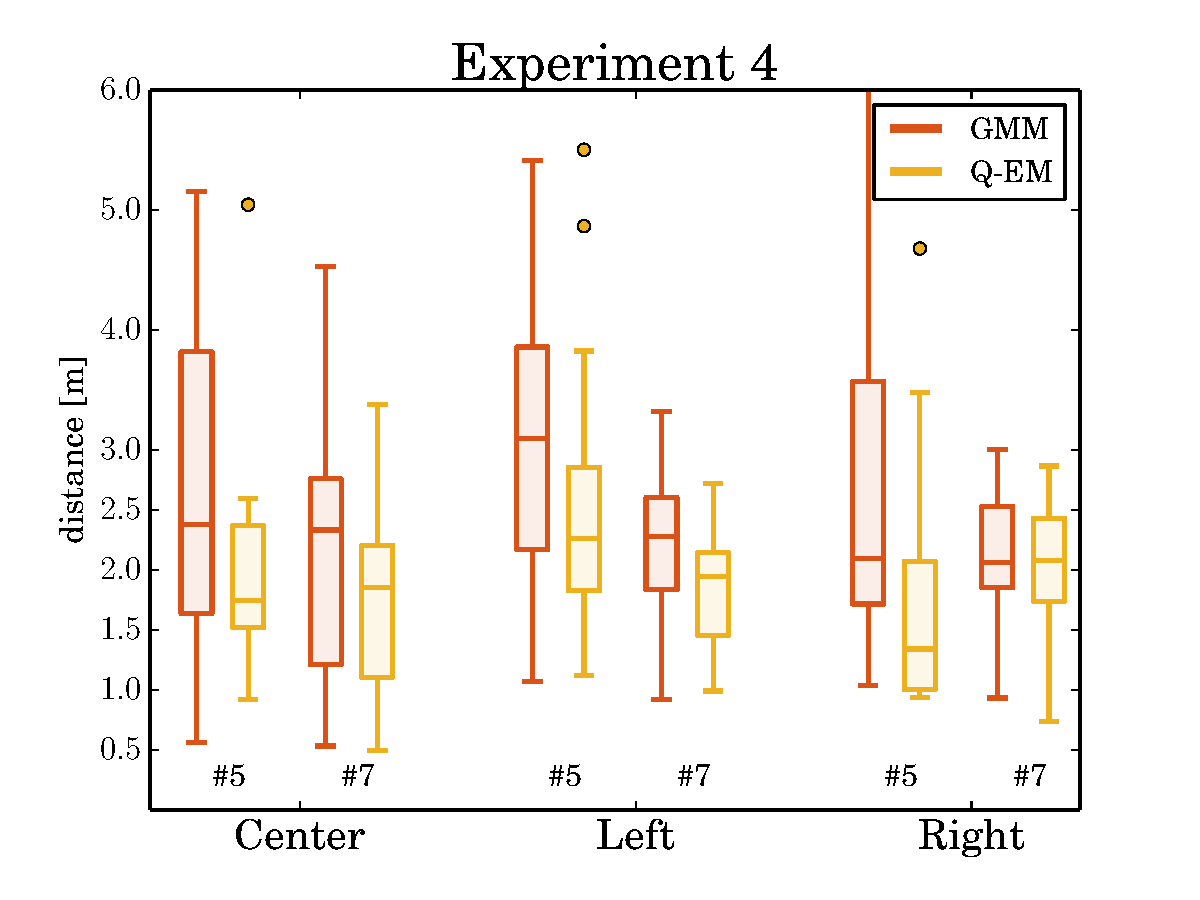
\includegraphics[width=0.445\textwidth]{./Figures/Results1/experiment4/experiment4.pdf}}
    \caption{Demonstrations of teacher \# 5. The teacher demonstrates a preference}
    \label{fig:subj_5_traj}
 \end{figure}
 
\begin{figure}
 \centering
 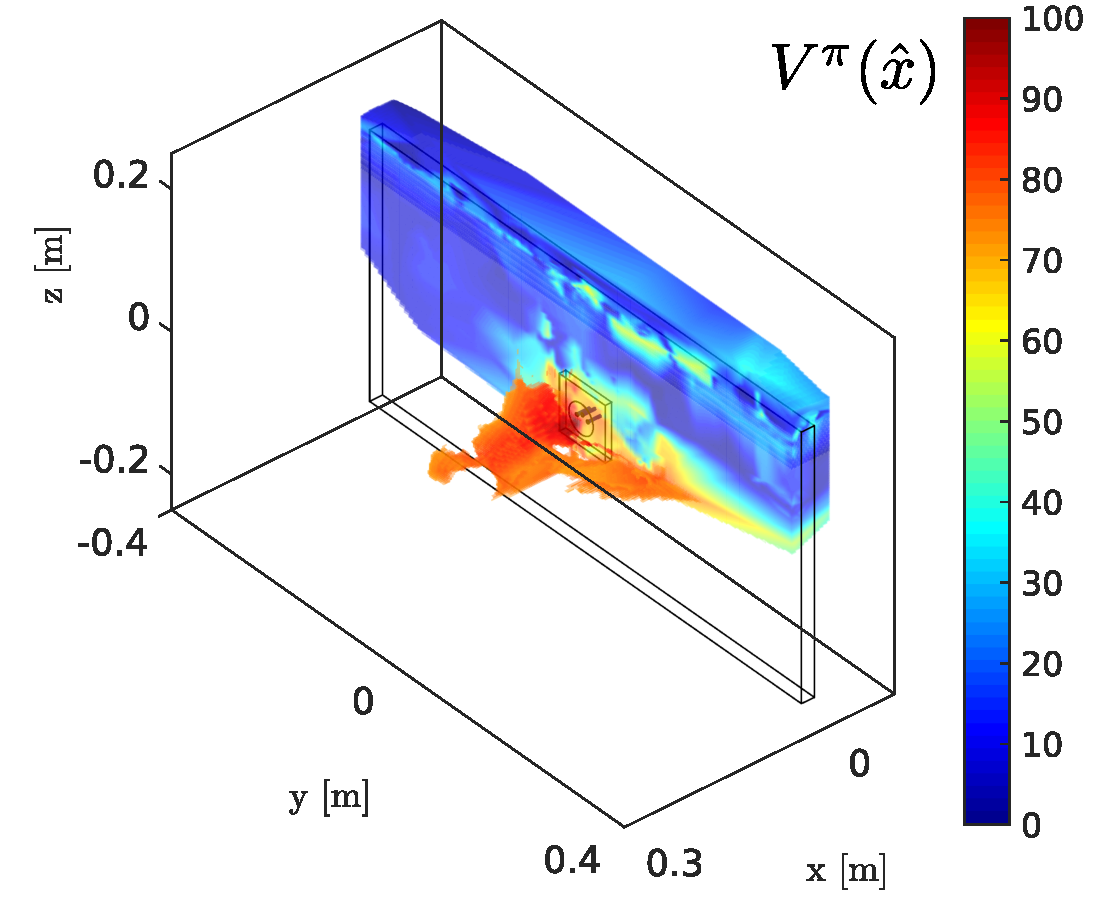
\includegraphics[width=0.8\textwidth]{./ch4-PiH/Figures/Fig/value_subj_5.pdf}
 \caption{Value function learned from the 15 demonstrations of teacher \#5. The value of the most likely state is plotted.}
 \label{fig:value_function_subj_5}
\end{figure}
 
 \begin{figure}
    \centering
    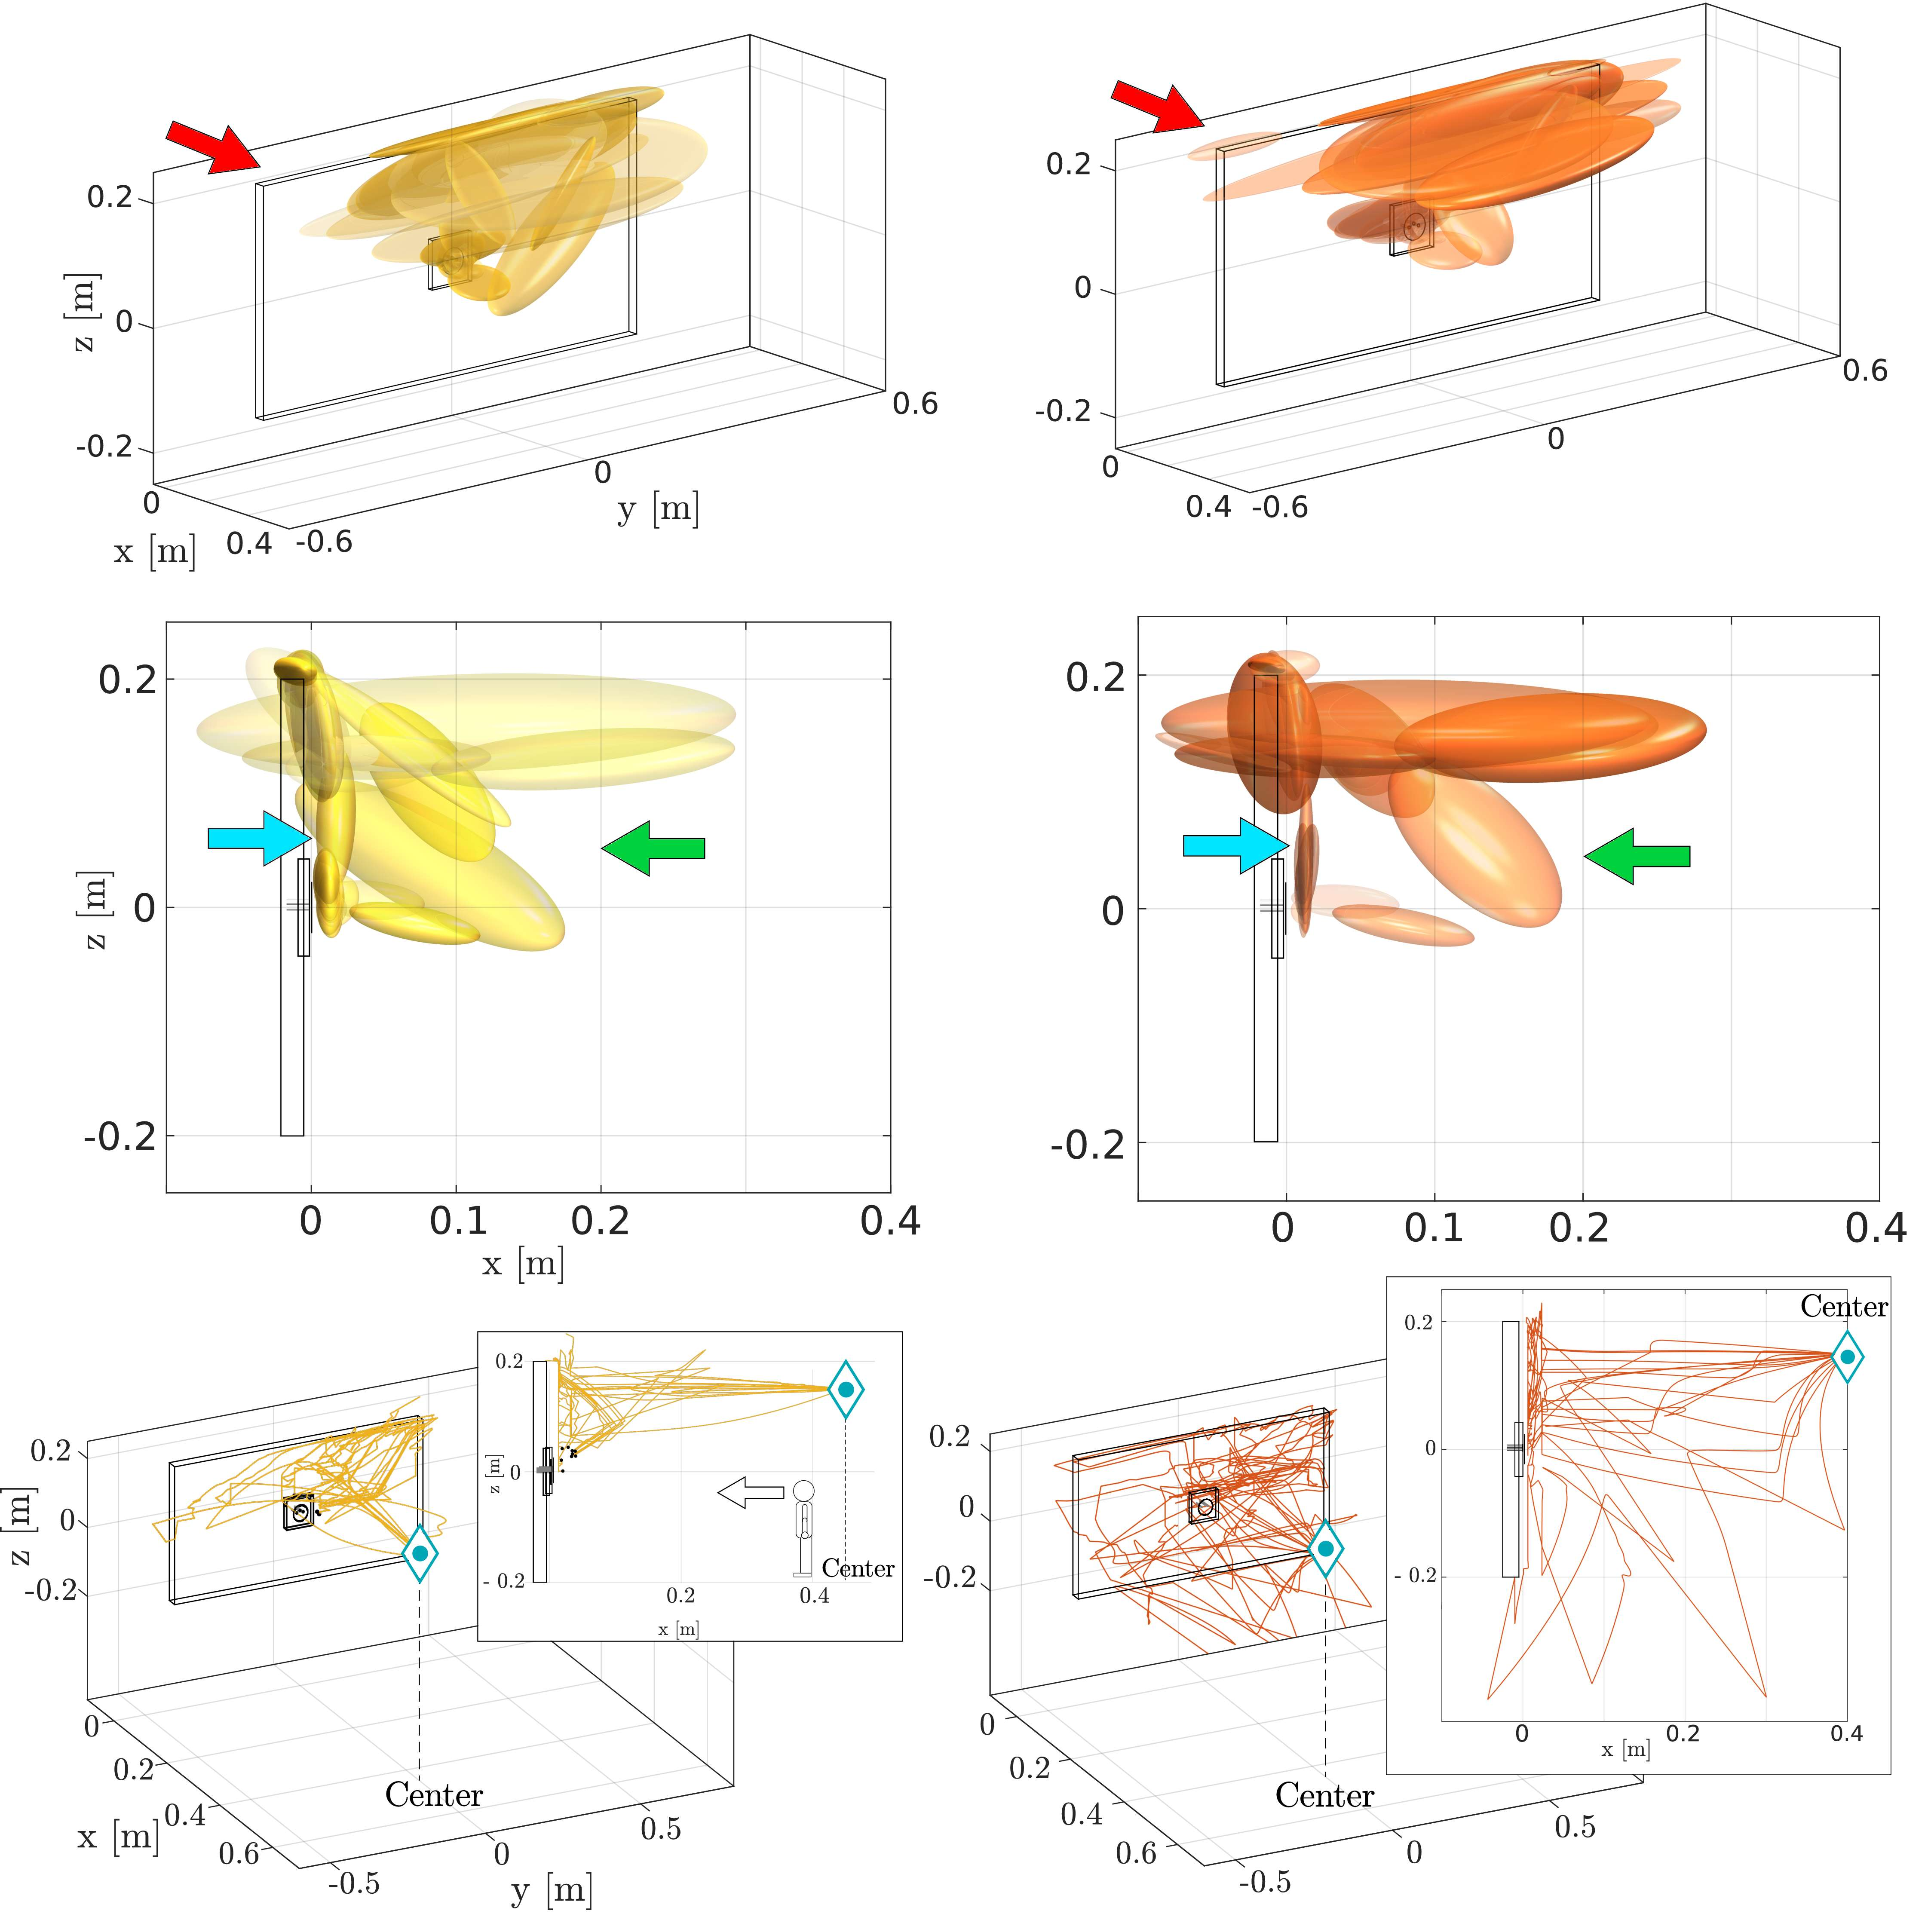
\includegraphics[width=\textwidth]{./ch4-PiH/Figures/Fig/gmm_v2c.pdf}
    \caption{Marginalised Gaussian Mixture parameters of the GMM and Q-EM learned from the demonstrations of teacher \#5. 
    The illustrated transparency of the Gaussian functions is proportional to their weight.
    \textit{Left column}: The Gaussian functions of the Q-EM have shifted from the left corner to the right. This is a result of the value function 
    being higher in the top right corner region, see Figure \ref{fig:value_function_subj_5}. \textit{Center column}:  The original data of the teacher 
    went quite far back which results in a Gaussian function given a direction which moves away from the wall (green arrow), whilst in the case
    of the Q-EM parameters this effect is reduced and moved closer towards the wall.  We can also see from the two plots of the Q-EM parameters 
    that they then follow the paths encoded by the value function.    
    \textit{Right column}: Rollouts of the policies learned from teacher \#5. We can see that trajectories from the GMM policy have not really 
    encoded a specific search patter, whilst the Q-EM policy gives many more consistent trajectories which replicate to some extent 
    the pattern of making a jump (no contact with the wall) from the top right corner to the socket's edge.}
    \label{fig:gmm_exp4}
\end{figure}
 
Figure \ref{fig:value_function_subj_5} illustrates the value function of the belief state learned from the data of teacher \# 5.
The states with the highest values seem to create a path going from the socket towards the right edge of the wall. 
We proceed as before to learn a GMM policy from the raw data and a Q-EM policy in which the data points are weighted by 
the gradient of the value function. In Figure \ref{fig:gmm_exp4}, we illustrate the 
resulting Marginalised Gaussian Mixture parameters for both the GMM and Q-EM policies and we plot 25 rollouts of each policy starting at 
the \textit{Center} initial condition used in Experiment 1. We note that the trajectories of the GMM 
policy have much variance in contrast to the Q-EM policy, resulting from an excess of variance in the 15 original demonstrations
given by the teacher. Too much variance is not necessarily good, a random (uniform) policy in terms of generated trajectories
will have the most variance and is as expected extremely inefficient in achieving a goal. Furthermore there is insufficient data to encode a pattern for the GMM model. In contrast, the Q-EM finds a 
pattern by combining multiple parts of the available data and as a result fewer data points are necessary to achieve a good policy. 
This effect is clear in Figure \ref{fig:experiment4_stats}, showing the performance of the GMM and Q-EM algorithms 
under the same initial conditions as in Experiment 1. For all the conditions and for both teachers \#5 and \#7 the Q-EM policy 
always does better than the GMM.

\begin{figure}
 \centering
 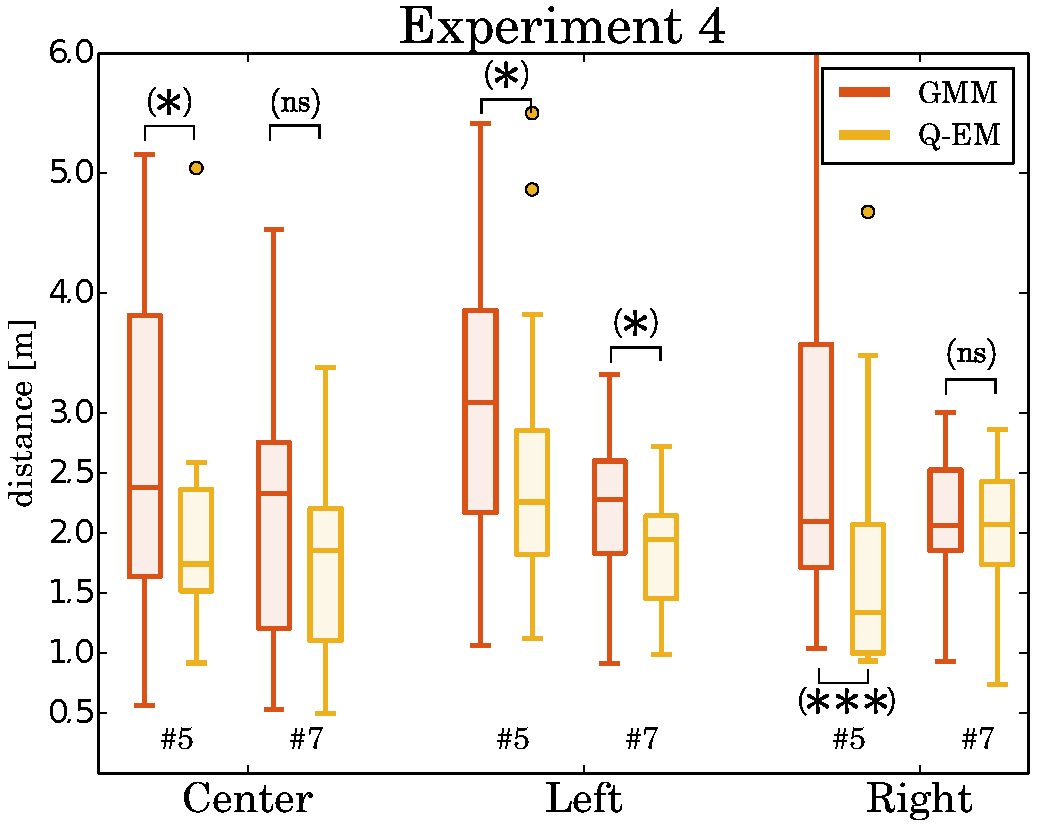
\includegraphics[width=0.8\textwidth]{./ch4-PiH/Figures/Fig/experiment4.pdf}
 \caption{Results of a GMM and Q-EM policy under the same test conditions as Experiment 1. The Q-EM policy nearly always does much better than the GMM policy.}
 \label{fig:experiment4_stats}
\end{figure}

We also tested whether we could use the Greedy policy as a means of gathering demonstrations in order to learn a value function and 
train a Q-Greedy policy. We used the Q-Greedy algorithm in combination with random perturbations applied to the Greedy velocity, to act as 
a simple exploration technique. We performed a maximum of 150 searches, which terminated once the socket was found and used these demonstrations to 
learn a value function and GMM policy which we refer to as Q-Greedy. Figure \ref{fig:three_searches} illustrates the statistical results 
of the Q-Greedy policy for Experiment 1 and 3, showing that there is no difference between two policies. 
Our exploration method is probably too simplistic to discover meaningful search patterns and we could probably devise better 
search strategies which would result in a good policy. However we have shown that human behaviour does already have a usable trade-off 
between exploration and exploitation which can be used to learn a new policy through our RL-PbD-POMDP framework.

\subsection{Generalisation}

An important aspect of a policy or any machine learning methodology is to be able to generalise. So far we have trained and 
evaluated our policy within the same environment. To test whether our GMM policies can generalise to a new setting we changed 
the location of the socket to the upper right corner of the wall. The GMM was trained in the frame of reference of the socket and
when we translated the socket's location it also translated the policy. 

\begin{figure}
 \centering
    \subfigure[]{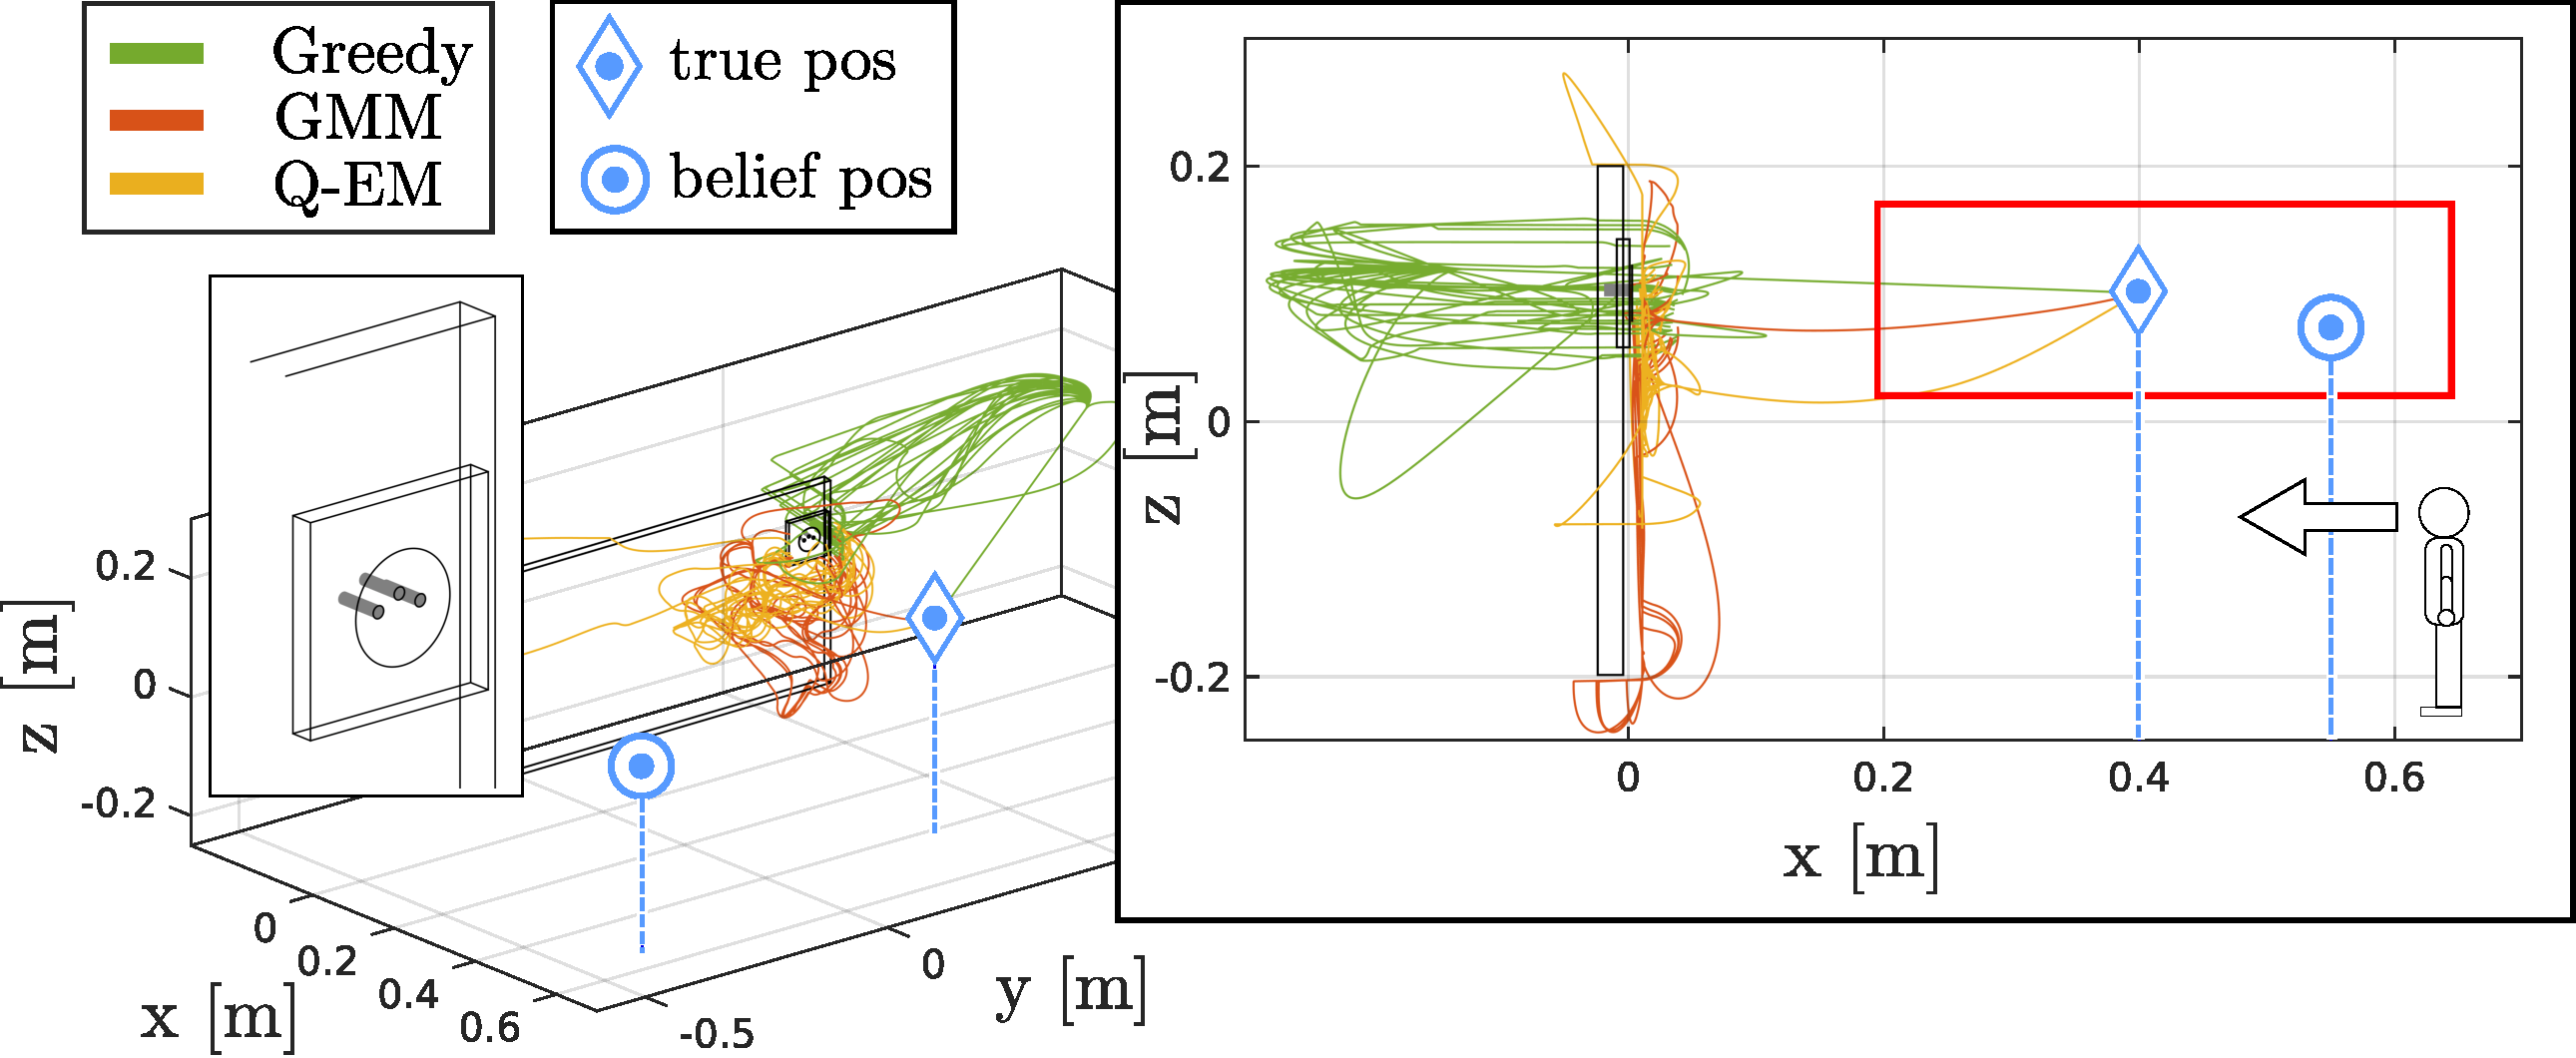
\includegraphics[width=\textwidth]{./ch4-PiH/Figures/Fig/traj_experiment5.pdf}}
    \caption{Evaluation of generalisation. The socket is located in at the top right corner of the wall. We consider a 
    \textit{Fixed} starting location for both the true and believed location of the end-effector. The red square depicts the 
    extent of the initial uncertainty, which is uniform. (b) Distance taken to reach the socket's edge. For the Fixed setup (see (a) for 
    the initial condition), both the Q-EM and GMM significantly outperform the Greedy. The other three conditions are the same as for 
    Experiment 1. }
    \label{fig:experiment5_traj}
\end{figure}

\begin{figure}
 \centering
    \subfigure[]{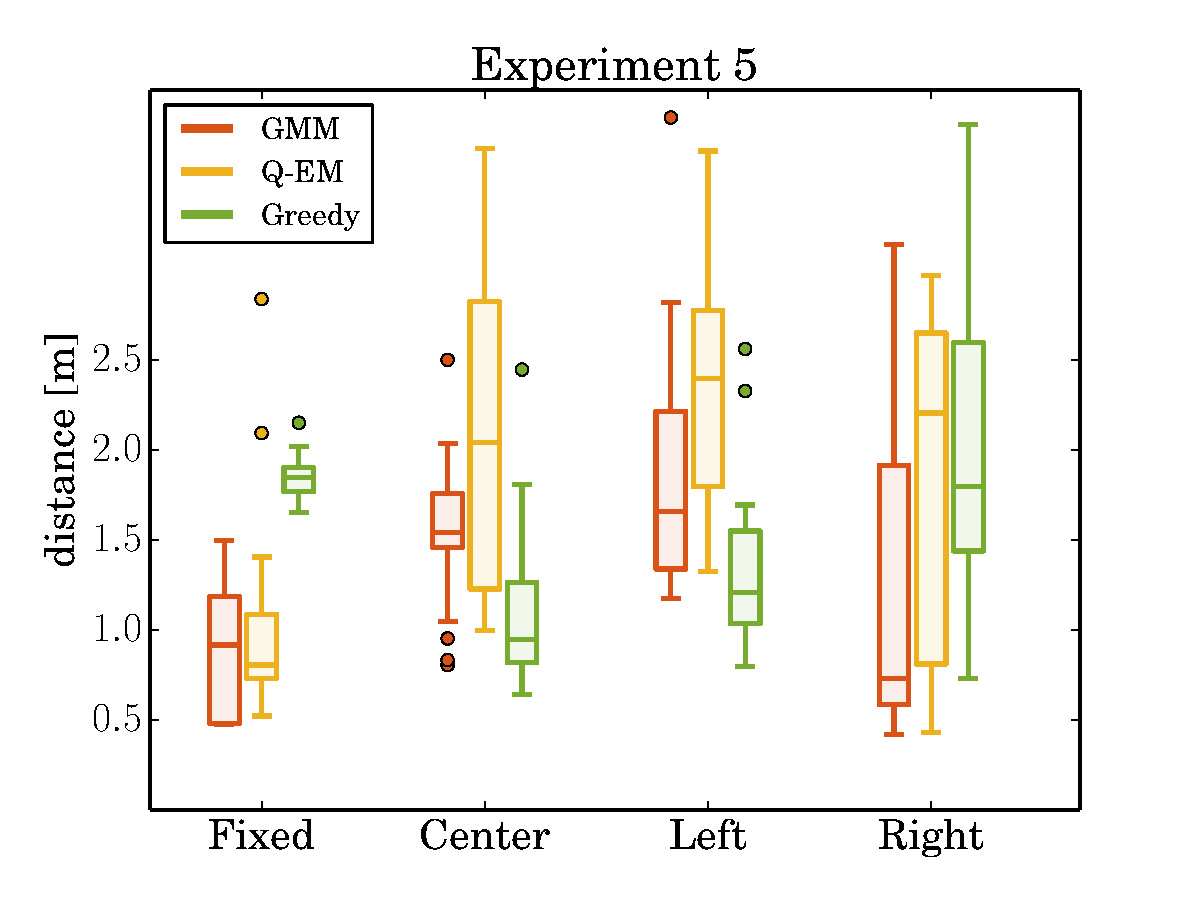
\includegraphics[width=0.8\textwidth]{./ch4-PiH/Figures/Fig/experiment5.pdf}}
    \caption{Distance taken to reach the socket's edge. For the Fixed setup (see Figure \ref{fig:experiment5_traj}) for 
    the initial condition), both the Q-EM and GMM significantly outperform the Greedy. }
    \label{fig:experiment5_stats}
\end{figure}

To evaluate the generalisation of our learned policy we use the same initial conditions of Experiment 1 with an additional 
new configuration named \textit{Fixed}, in which both the true and believed location are fixed, blue triangle and circle.
Figure \ref{fig:experiment5_traj} illustrates the trajectories of the three search policies for the \textit{Fixed} initial condition. 
The Greedy policy moves in a straight line towards the top
right corner of the table. As the true position is to the right, it takes the Greedy policy longer to find the wall 
in contrast to both the GMM and Q-EM policies. From the statistical results shown in Figure \ref{fig:experiment5_stats} we can see
that for the \textit{Fixed} and \textit{Right} initial condition, which are similar, both GMM and Q-EM are better. However, for 
the \textit{Center} and \textit{Left} initial condition this is no longer the case. 
The Greedy method is better under this condition since the socket is close to informative features (it is located close to the edges of the wall). 
Once the end-effector has entered in contact with the wall the actions of the Greedy policy always result in a decrease of uncertainty, which was not the case when the socket was located in the center of wall. 
Thus in both the \textit{Fixed} and \textit{Right} initial condition the Greedy method does worse because it takes longer
to find the wall.

The GMM based policies are still able to generalise under different socket locations. In general, as the socket's location is moved 
further from the original frame of reference in which it was learned, the higher is the likelihood that the search quality degrades. We 
chose the upper right corner since it is the furthest point from the origin and the GMM and Q-EM policies were still able to find 
the socket. We note that the policy will always be able to find the socket once it has localised itself. This can be seen from the vector field 
of the GMM policy when the uncertainty is low, see Figure \ref{fig:policy_vf} on page \pageref{fig:policy_vf}. In this case the policy is a sink function 
with a single point attractor.

\subsection{Distance taken to connect the plug to the socket}
% Real socket experiment.
% Show initial condition setup with belief. (the experiment)
In this section we evaluate the distance taken for the policies and humans to establish a connection, after the socket 
has been found. We start measuring the distance 
from the point that the plug enters in contact with the socket's edge until the plug is connected to the socket. All the following evaluations are done 
on a KUKA LWR4 robot. The robot's end-effector is equipped with a plug holder on which is attached a force-torque sensor, 
the same holders used during the demonstration of the human teachers. In this way both the teacher and robot apprentice share 
the same sensory interface.

We chose to have the robot's end-effector located to the right of the socket and a belief spread uniformly 
along the z-axis. See Figure \ref{fig:real_pictures} for an illustration of the initial starting condition.
This initial configuration was used to evaluate the search policies for the three different sockets, see Figure \ref{fig:search_task_setup} 
on page \pageref{fig:search_task_setup} for an illustration of the sockets. The same initial configuration for 
the evaluation of the three sockets was kept in order to observe the generalisation properties of the policies. 
As a reminder we used only the training data from demonstrations acquired during the search with socket A. Socket B has a funnel which should make it 
easier to connect whilst socket C should be more difficult as it has no informative features on its surface. 

For each of the sockets we performed 25 searches starting from the same initial condition. In Figure \ref{fig:real_policy} we plot
the trajectories of each of the search methods for socket A. The GMM reproduces some of the behaviour exhibited by humans, such as 
first localising itself at the top of the socket before trying to attempt to make a connection. The Q-EM algorithm exhibits less variation
than the GMM and tends to pass via the bottom of the socket to establish a connection. The Greedy method in contrast is much more  
stochastic since it does not take into consideration the variance of the uncertainty but tries instead to directly establish a connection.
Figure \ref{fig:real_statistics} (c) shows that for socket A both the Greedy and Q-EM are better than the GMM and the Q-EM has less
variance in comparison to the Greedy searches.  All three search methods are vastly superior, when compared to the human's performance 
see Figure \ref{fig:real_statistics}.  In Figure \ref{fig:real_pictures} illustrates a typical rollout of the GMM search policy for both 
socket A and C. Once a contact is made with the socket's edge the policy tends to stay close to informative features and tends to 
wander vertically up and down. Only when the uncertainty has been reduced does the GMM policy try to go towards the socket's connector. 

\begin{figure}
 \centering
    \subfigure[]{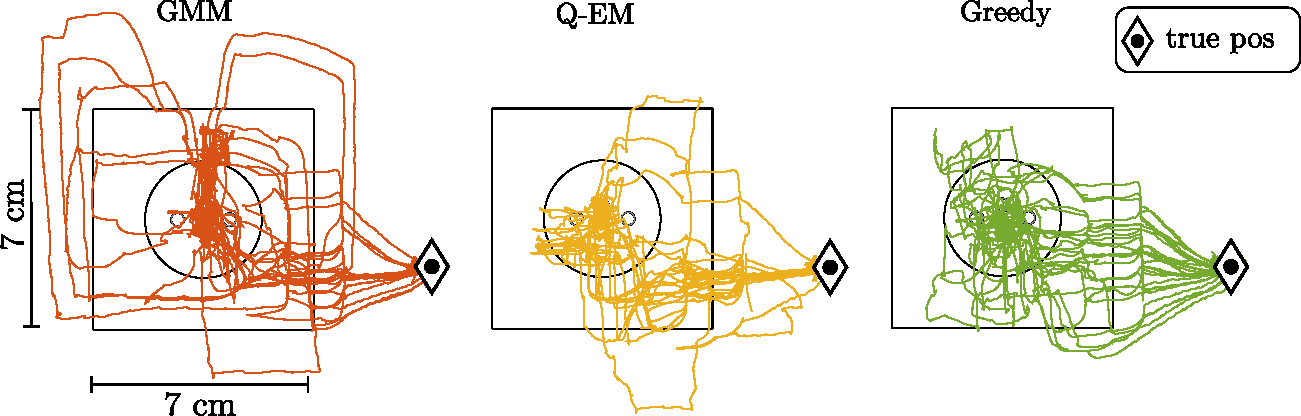
\includegraphics[width=\textwidth]{./ch4-PiH/Figures/Results2/socket_connection_A.pdf}}
    \caption{%(a) All three sockets have the same connector interface, but have different structures. Both 
   % socket A and B have an edge around the center whilst the surface of socket C is featureless and more elevated than the other two. 
    25 search trajectories for each of the three search policies for socket A. }
    \label{fig:real_policy}
\end{figure}


\begin{figure*}
 \centering
 \subfigure[]{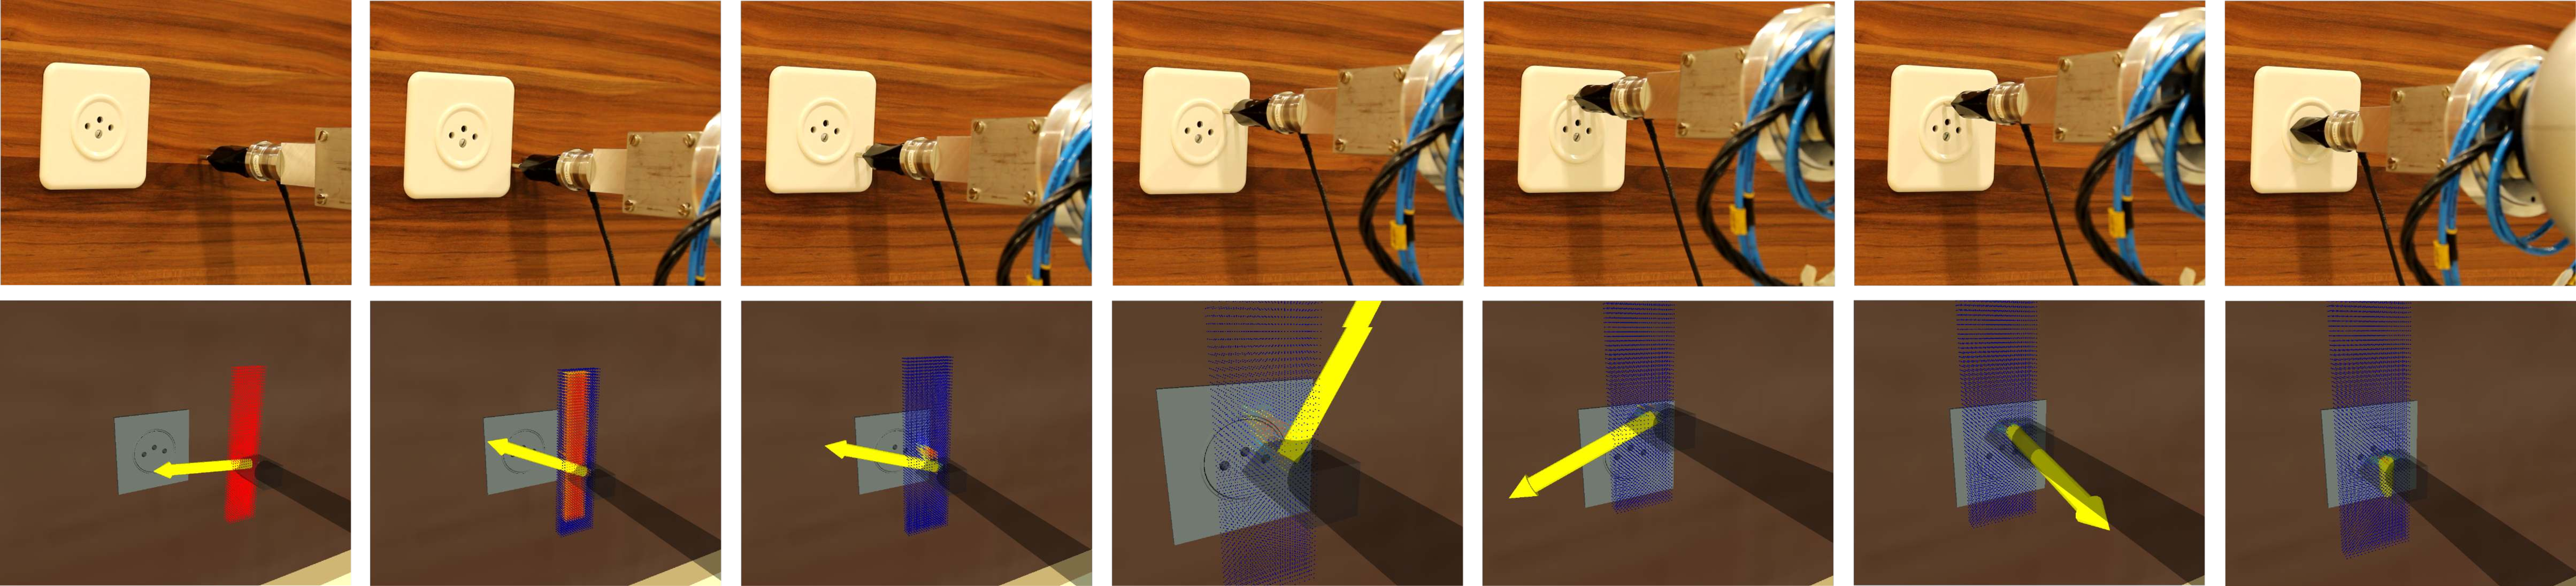
\includegraphics[width=0.95\textwidth]{./ch4-PiH/Figures/Results2/s1_sequence.pdf}}
 \subfigure[]{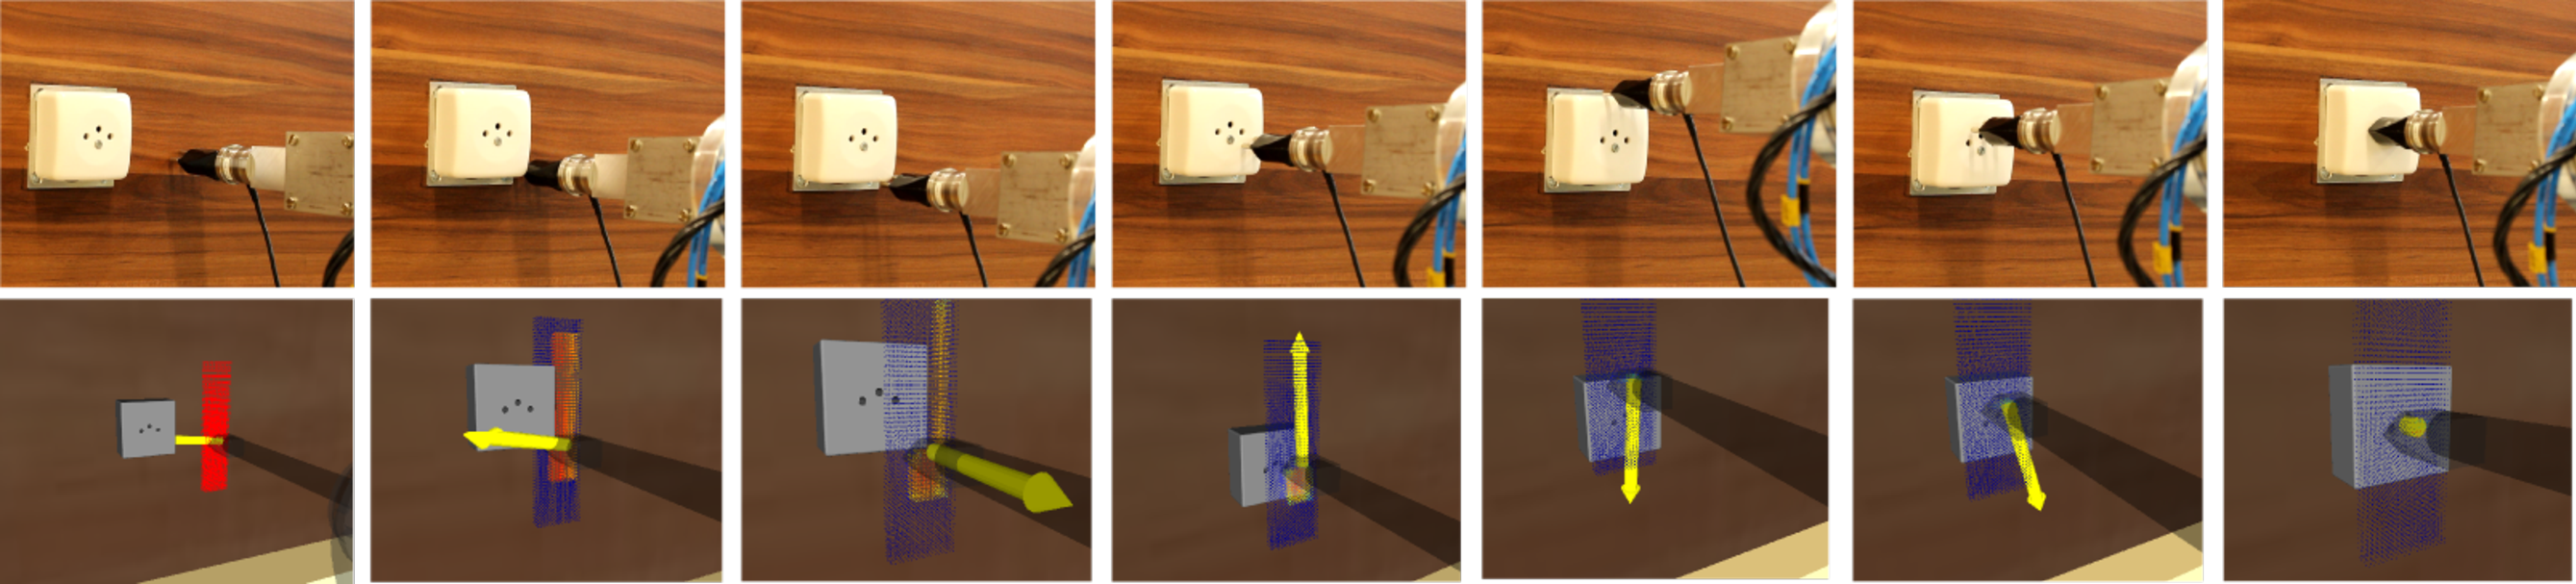
\includegraphics[width=0.95\textwidth]{./ch4-PiH/Figures/Results2/s2_sequence.pdf}}
 \caption{KUKA LWR4 equipped with a holder mounted with a ATI 6-axis force-torque sensor. (a) The robot's end-effector starts to the 
 right of socket A. The second row shows screen captures taken of ROS Rviz data visualiser in which we see the Point Mass Filter 
 (red particles) and a yellow arrow indicating the direction given by the policy. In this particular run, the plug remained in contact with the ring of the socket until 
 the top was reached before making a connection. (b) Same initial condition as in (a) but with socket C. The policy leads the plug down to 
 the bottom corner of the socket before going the center of the top edge, localising itself, and then making a connection.}
 \label{fig:real_pictures}
\end{figure*}

\begin{figure}
 \centering
   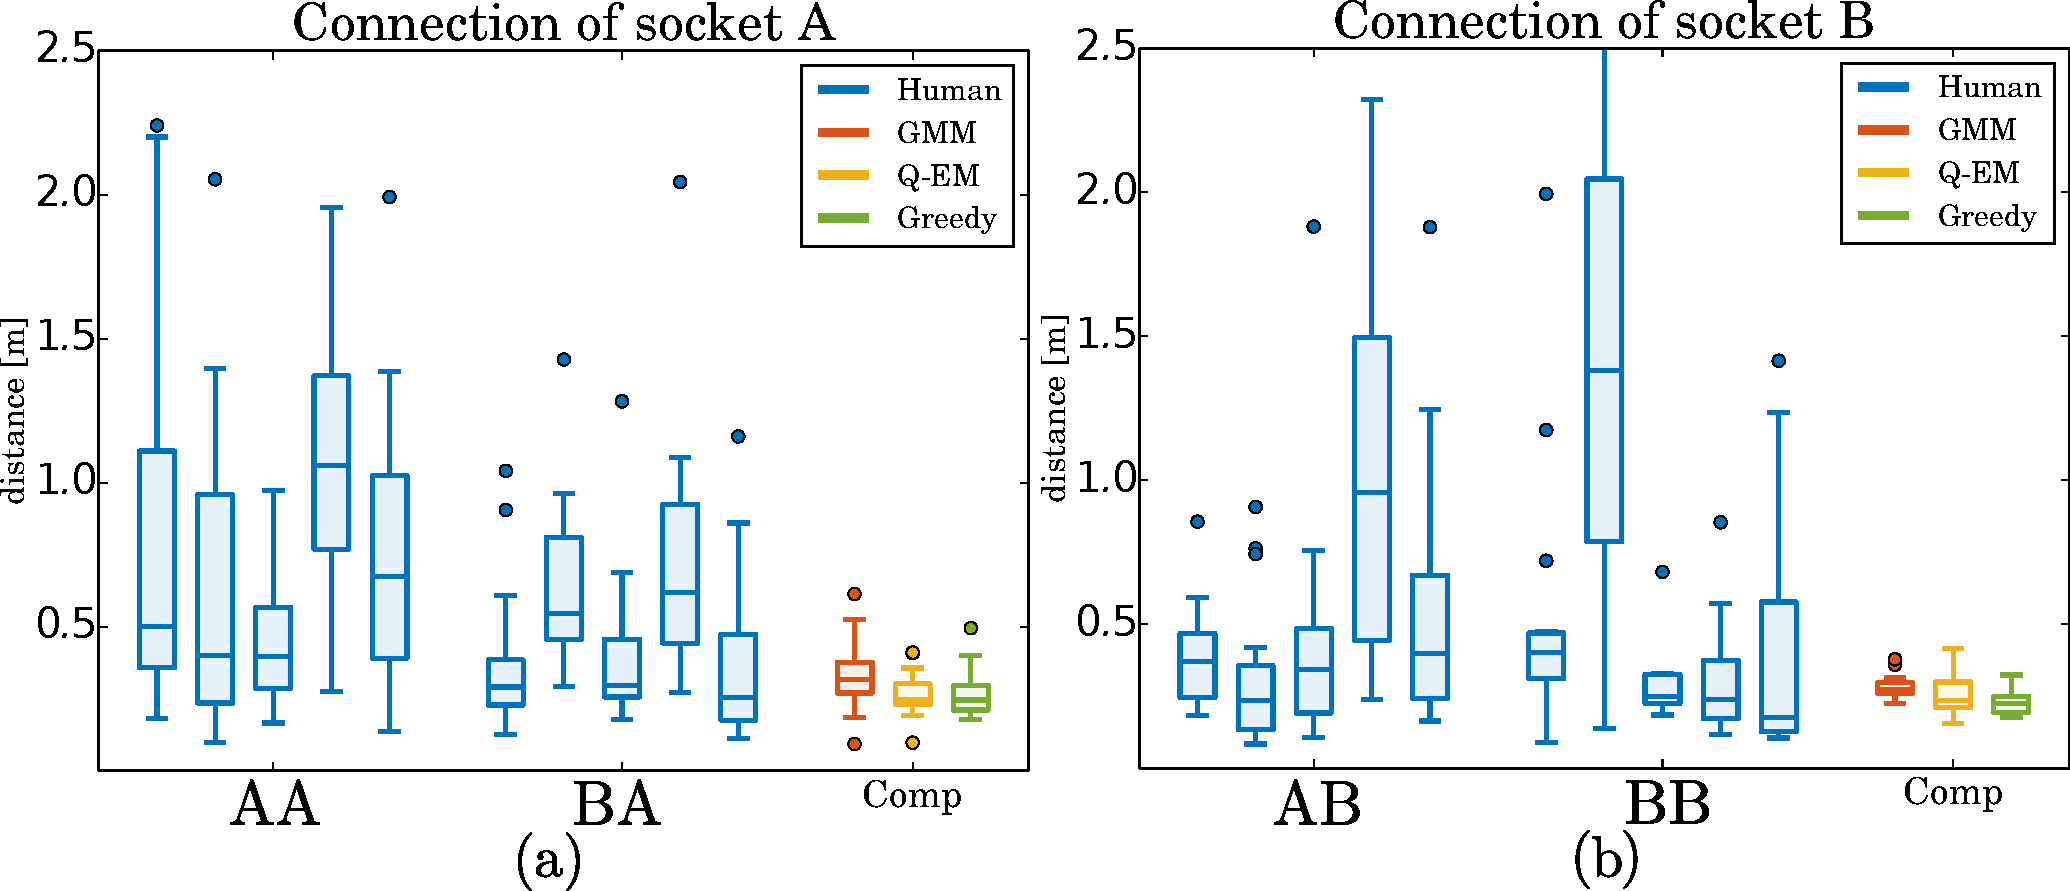
\includegraphics[width=\textwidth]{./ch4-PiH/Figures/Results2/real_exp_socketAB.pdf}
  % \subfigure[]{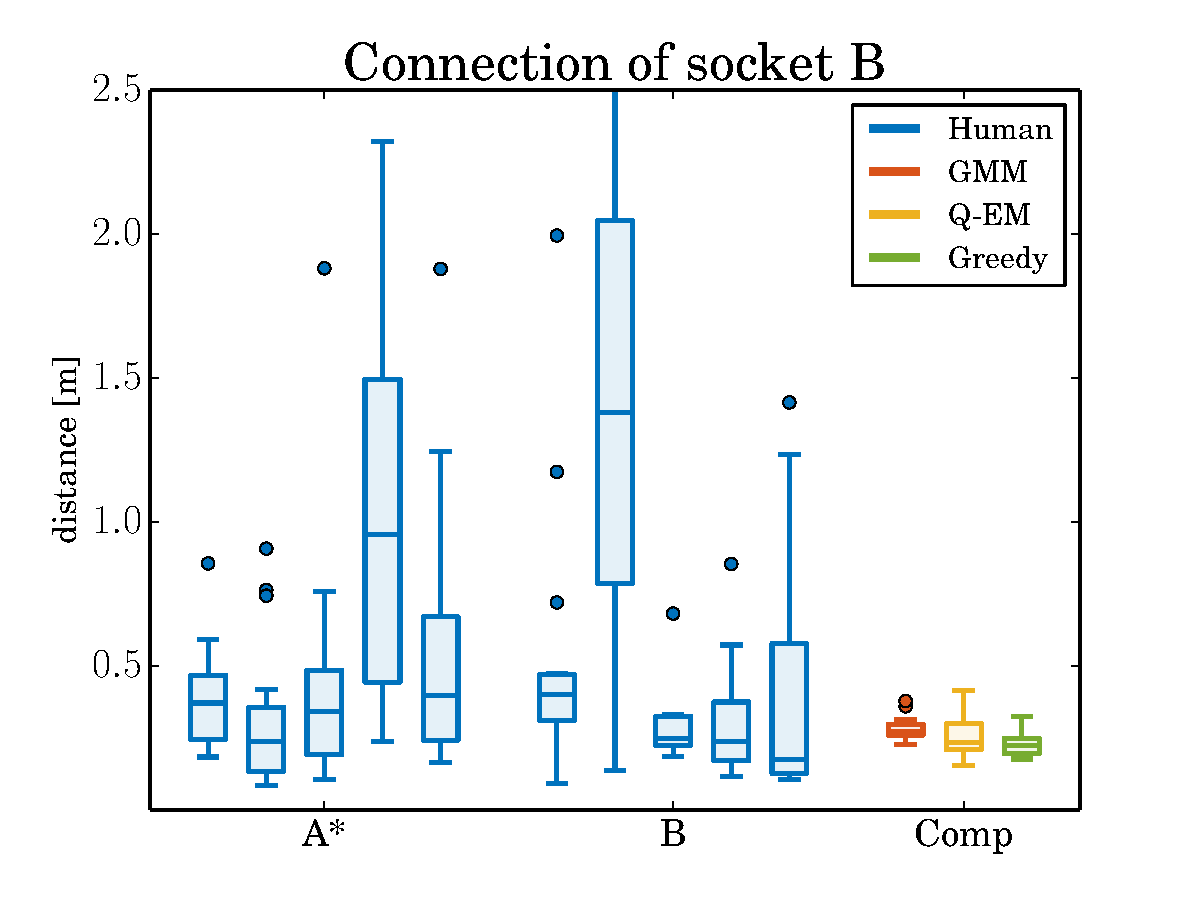
\includegraphics[width=0.3\textwidth]{./ch4-PiH/Figures/Results2/real_exp_socketB.pdf}}
  % \subfigure[]{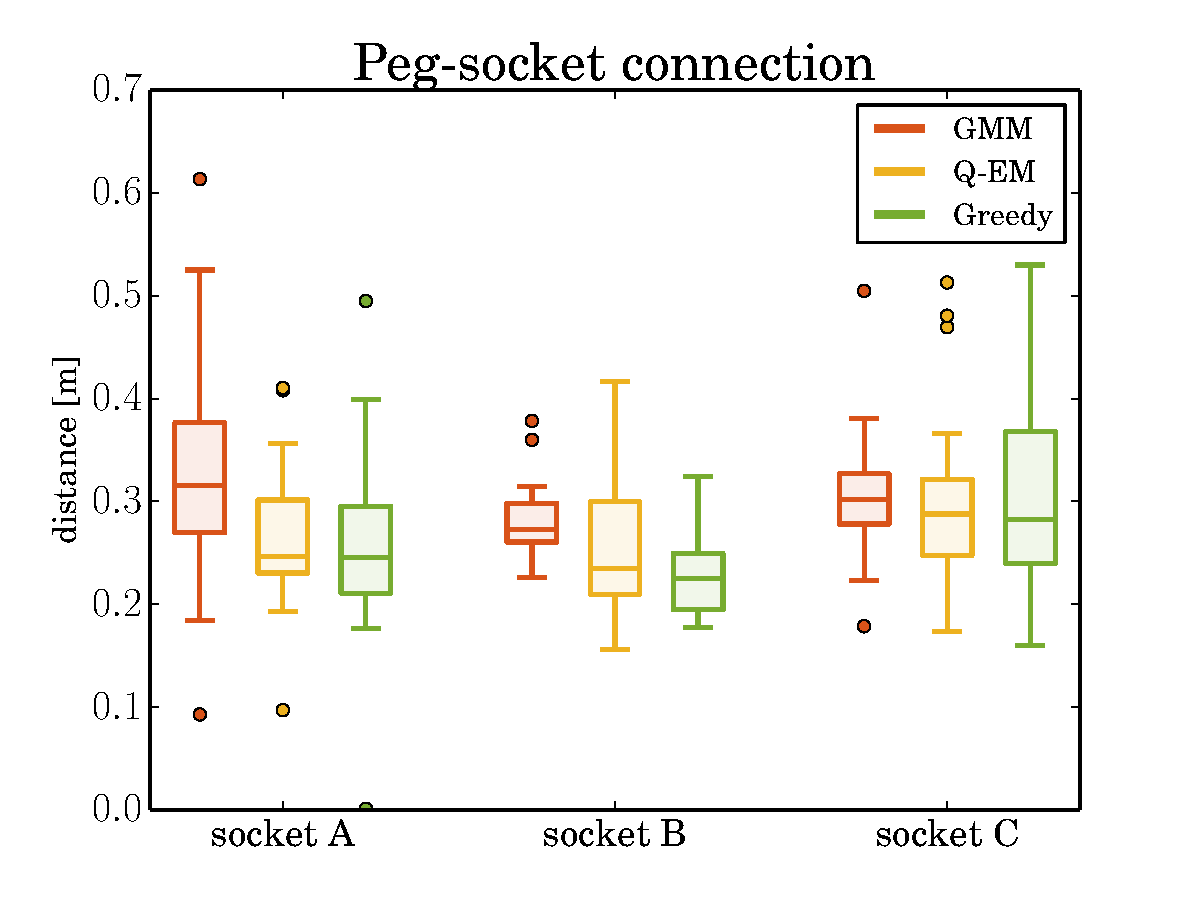
\includegraphics[width=0.3\textwidth]{./ch4-PiH/Figures/Results2/peg_socket_connection.pdf}}
  \caption{Distance taken to connect plug to socket once the socket is localised. (a) \textbf{Socket A}. The human 
  Group A are the set of teachers who first started with socket A. They had no previous training on another socket beforehand. Group 
  BA first gave demonstrations on Socket B before giving demonstrations on Socket A. Group BA
  is better than Group AA at doing the task. This is most likely a training effect. However all policy search methods are far better
  at connecting the plug to the socket. (b) \textbf{Socket B}. Both Groups AB and BB are similar in terms 
  of the distance they took to insert the plug into the socket and as was the case for (a), the search policies travel less to accomplish 
  the task.   } 
  \label{fig:real_statistics}
\end{figure}

\begin{figure}
 \centering
   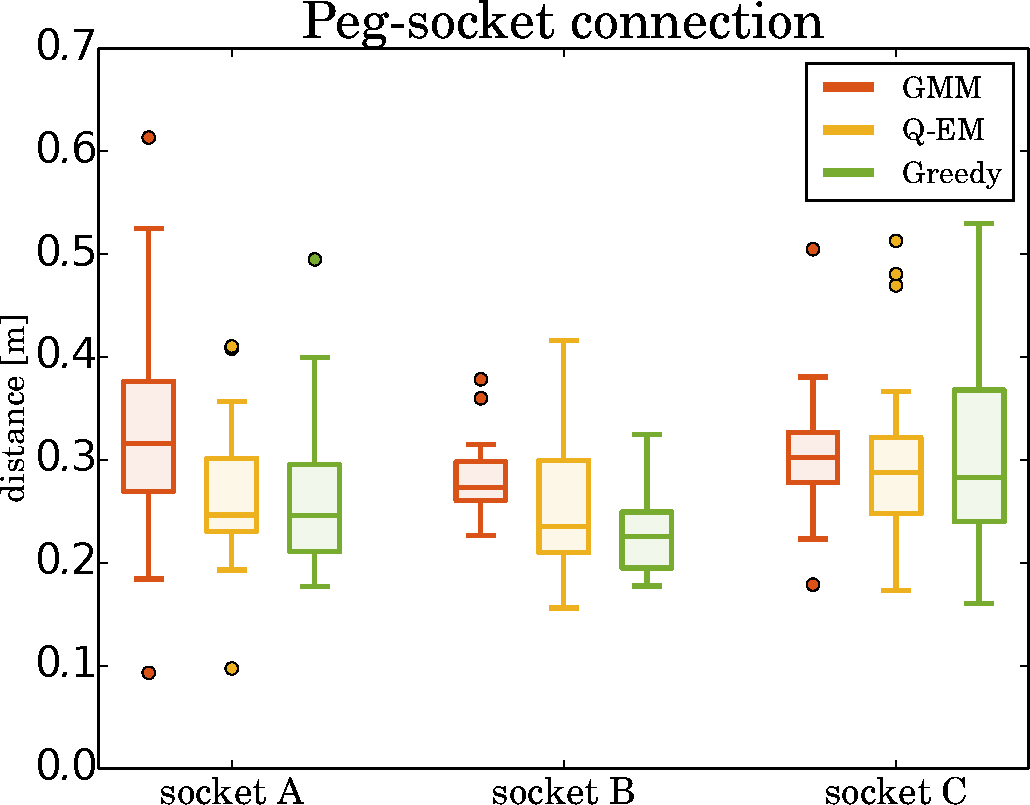
\includegraphics[width=0.8\textwidth]{./ch4-PiH/Figures/Results2/peg_socket_connection_v2.pdf}
   \caption{Distance taken (measured from point of contact of plug with socket edge) to connect the plug to the socket.}
  \label{fig:real_statistics2}
\end{figure}

The GMM and Q-EM policies are able to generalise to both socket B and C, as the geometric shape and connector interface of the 
two sockets are similar to socket A. The local force modulation of the policy's vector field, which is not learned, allows the 
end-effector to surmount edges and obstacles whilst trying to maintain a constant contact force in the x-axis. This modulation makes it possible for the plug to get on top of socket C.
Figure \ref{fig:real_statistics} (c) illustrates the statistics of the distance taken to establish a connection for all three sockets. 
The interesting point is that both the GMM and Q-EM algorithms perform better than the Greedy approach for socket C. Socket C has no informative 
features on its surface and as a result myopic policies such as the Greedy policy will perform poorly. However for socket A 
and B, the Greedy policy performs better as both of these sockets have edges around their connector point allowing for easy localisation. 
It can also be seen that most search methods perform better on socket B than A, since the funnel shape connector helps in maintaining the plug 
within the vicinity of the socket's holes. 


The discrepancy between the humans performance and the search policies can be attributed to many causes. One plausible reason is 
that the PMF probability density representation of the belief is more accurate than the human teachers position belief. 
Also, the motion noise parameter was fixed to be proportional to the velocity and the robot moves at gentle pace ($\sim1$ cm/s) as 
opposed to some of the human teachers. In actuality, humans are far less precise than the KUKA which has sub-millimetre accuracy.

\section{Discussion \& Conclusion}\label{ch4:conclusion}
% Recapulate what we did 
%
% We learned a 
%
%

In this work we learned search policies from demonstrations provided by human teachers for a task
which consisted of first localising a power socket (either socket A, B or C) and then connecting it with a plug. Only haptic information 
was available as the teachers were blindfolded. We made the assumption that the position belief of the human teachers 
was initially uniformly distributed in a fixed rectangular region of which they were 
informed and is considered prior knowledge. All subsequent beliefs were then updated in a Bayesian recursion 
using the measured velocity obtained from a vision tracking system, and wrench acquired from a force torque sensor attached 
to the plug. The filtered probability density function, represented by a Point Mass Filter, was then compressed to the 
most likely state and entropy.

Two Gaussian Mixture Model policies were learned from the data recorded during the human teachers' demonstrations. 
The first policy, called Q-EM, was learned in an Actor-Critic RL framework in which a value function was learned over 
the belief space. This was then used to weight training datapoints in the M-step update of Expectation-Maximisation (EM). The second 
policy, called GMM, was learned using the standard EM algorithm, and considered all training data points equally,
following in the footsteps of our initial approach \cite{Chambrier2014}. Both the Q-EM and GMM policies were trained 
with data solely from the demonstrations of the search with socket A.

We evaluated 4 different aspects of the learned policies. Firstly, we evaluated which of three policies, Q-EM, GMM and a Greedy policy, 
took the least distance to find the socket. We concluded that across three different Experiments the Q-EM algorithm always performed
the best. It was clear that the Q-EM policy was less random and more consistent than the GMM policy as it tried to enter in 
contact with the wall at the same height as the socket thus increasing the chances of finding the socket.

Secondly, we tested the importance of the data provided by the human teachers. We took the worst two teachers and trained an
individual GMM and Q-EM policy for each of them. We found that the performance of the Q-EM was better than the GMM in terms 
of distance travelled to find the socket. When qualitatively evaluating the trajectories of the GMM with respect to the 
Q-EM for the worst teacher, it is clear that the Q-EM policy managed to extract a search pattern, which was not the case 
for the GMM policy. We also tried to learn a Q-EM policy from the data provided by a Greedy policy with explorative noise 
and we found no improvement. From these results we conclude that the exploration and exploitation aspects of the trajectories 
provided by the human teachers is necessary.

Thirdly, we tested whether the two policies (GMM and Q-EM) were able to generalise to a different socket location. Under a specific condition,
which we called \textit{Fixed}, both policies were significantly better than the Greedy policy. However for the \textit{Center}
and \textit{Left} initial conditions the Greedy policy performed better. For the initial conditions in which the Greedy policy 
enters in contact with the wall at an early stage, it also performs better than the GMM and Q-EM. The reason for this is that  
the actions taken by the Greedy policy in this setting will always result in a decrease of entropy when the location
of the socket is close to a corner, as opposed to being in the center of the wall.

Fourthly, we evaluated all three policies on the KUKA LWR4 robot and found that all the policies did better than the human 
teachers. For socket A, on which both the GMM and Q-EM policies were trained, there is no clear distinction between 
the Q-EM and Greedy policy. On socket B, which was novel, the Greedy policy performed better than the statistical controllers, 
which we hypothesize was a result of a funnel which would make it easier for a myopic policy. For socket C, both the 
GMM and Q-EM policies performed better than the Greedy, as socket C has no features on its surface, this being a disadvantage 
for a myopic policy.

We conclude by making the observation that by simply adding a binary reward function in combination with 
data provided by human demonstrations, with Fitted reinforcement learning, we can learn a better policy without 
the need to perform expensive exploration-exploitation rollouts traditionally associated with reinforcement learning and 
designing complicated reward functions. This is especially advantageous when only a few demonstrations are available.
